\documentclass[]{book}
\usepackage{lmodern}
\usepackage{amssymb,amsmath}
\usepackage{ifxetex,ifluatex}
\usepackage{fixltx2e} % provides \textsubscript
\ifnum 0\ifxetex 1\fi\ifluatex 1\fi=0 % if pdftex
  \usepackage[T1]{fontenc}
  \usepackage[utf8]{inputenc}
\else % if luatex or xelatex
  \ifxetex
    \usepackage{mathspec}
  \else
    \usepackage{fontspec}
  \fi
  \defaultfontfeatures{Ligatures=TeX,Scale=MatchLowercase}
\fi
% use upquote if available, for straight quotes in verbatim environments
\IfFileExists{upquote.sty}{\usepackage{upquote}}{}
% use microtype if available
\IfFileExists{microtype.sty}{%
\usepackage{microtype}
\UseMicrotypeSet[protrusion]{basicmath} % disable protrusion for tt fonts
}{}
\usepackage[margin=1in]{geometry}
\usepackage{hyperref}
\hypersetup{unicode=true,
            pdftitle={Biology II Laboratory Manual},
            pdfauthor={Nikolaus Sucher},
            pdfborder={0 0 0},
            breaklinks=true}
\urlstyle{same}  % don't use monospace font for urls
\usepackage{booktabs}

\usepackage{graphicx,grffile}
\makeatletter
\def\maxwidth{\ifdim\Gin@nat@width>\linewidth\linewidth\else\Gin@nat@width\fi}
\def\maxheight{\ifdim\Gin@nat@height>\textheight\textheight\else\Gin@nat@height\fi}
\makeatother
% Scale images if necessary, so that they will not overflow the page
% margins by default, and it is still possible to overwrite the defaults
% using explicit options in \includegraphics[width, height, ...]{}
\setkeys{Gin}{width=\maxwidth,height=\maxheight,keepaspectratio}
\IfFileExists{parskip.sty}{%
\usepackage{parskip}
}{% else
\setlength{\parindent}{0pt}
\setlength{\parskip}{6pt plus 2pt minus 1pt}
}
\setlength{\emergencystretch}{3em}  % prevent overfull lines
\providecommand{\tightlist}{%
  \setlength{\itemsep}{0pt}\setlength{\parskip}{0pt}}
\setcounter{secnumdepth}{5}
% Redefines (sub)paragraphs to behave more like sections
% \ifx\paragraph\undefined\else
% \let\oldparagraph\paragraph
% \renewcommand{\paragraph}[1]{\oldparagraph{#1}\mbox{}}
% \fi
% \ifx\subparagraph\undefined\else
% \let\oldsubparagraph\subparagraph
% \renewcommand{\subparagraph}[1]{\oldsubparagraph{#1}\mbox{}}
% \fi

%%% Use protect on footnotes to avoid problems with footnotes in titles
\let\rmarkdownfootnote\footnote%
\def\footnote{\protect\rmarkdownfootnote}

%%% Change title format to be more compact
\usepackage{titling}

% Create subtitle command for use in maketitle
\newcommand{\subtitle}[1]{
  \posttitle{
    \begin{center}\large#1\end{center}
    }
}

\setlength{\droptitle}{-2em}
  \title{Biology II Laboratory Manual}
  \pretitle{\vspace{\droptitle}\centering\huge}
  \posttitle{\par}
  \author{Nikolaus Sucher}
  \preauthor{\centering\large\emph}
  \postauthor{\par}
  \date{}
  \predate{}\postdate{}


\usepackage[raggedright]{titlesec}


\usepackage[bf,singlelinecheck=off]{caption}
\usepackage{siunitx}
\usepackage{framed}
\usepackage{xcolor}
 \definecolor{shadecolor}{RGB}{248,248,248}
\usepackage{grffile}
\usepackage{graphicx}
\usepackage{morefloats}
\usepackage{parskip}
 \setlength{\parindent}{15pt}

%\renewcommand{\textfraction}{0.05}
%\renewcommand{\topfraction}{0.8}
%\renewcommand{\bottomfraction}{0.8}
%\renewcommand{\floatpagefraction}{0.75}

\renewenvironment{quote}{\begin{VF}}{\end{VF}}
\let\oldhref\href
\renewcommand{\href}[2]{#2\footnote{\url{#1}}}

\ifxetex
  \usepackage{letltxmacro}
  \setlength{\XeTeXLinkMargin}{1pt}
  \LetLtxMacro\SavedIncludeGraphics\includegraphics
  \def\includegraphics#1#{% #1 catches optional stuff (star/opt. arg.)
    \IncludeGraphicsAux{#1}%
  }%
  \newcommand*{\IncludeGraphicsAux}[2]{%
    \XeTeXLinkBox{%
      \SavedIncludeGraphics#1{#2}%
    }%
  }%
\fi

\makeatletter
\newenvironment{kframe}{%
\medskip{}
\setlength{\fboxsep}{.8em}
 \def\at@end@of@kframe{}%
 \ifinner\ifhmode%
  \def\at@end@of@kframe{\end{minipage}}%
  \begin{minipage}{\columnwidth}%
 \fi\fi%
 \def\FrameCommand##1{\hskip\@totalleftmargin \hskip-\fboxsep
 \colorbox{shadecolor}{##1}\hskip-\fboxsep
     % There is no \\@totalrightmargin, so:
     \hskip-\linewidth \hskip-\@totalleftmargin \hskip\columnwidth}%
 \MakeFramed {\advance\hsize-\width
   \@totalleftmargin\z@ \linewidth\hsize
   \@setminipage}}%
 {\par\unskip\endMakeFramed%
 \at@end@of@kframe}
\makeatother

\newenvironment{Shaded}{\begin{kframe}}{\end{kframe}}

\newenvironment{rmdblock}[1]
  {
  \begin{itemize}
  \renewcommand{\labelitemi}{
    \raisebox{-.7\height}[0pt][0pt]{
      {\setkeys{Gin}{width=3em,keepaspectratio}\includegraphics{images/#1}}
    }
  }
  \setlength{\fboxsep}{1em}
  \begin{kframe}
  \item
  }
  {
  \end{kframe}
  \end{itemize}
  }

\newenvironment{rmdnote}
  {\begin{rmdblock}{note}}
  {\end{rmdblock}}

\newenvironment{rmdcaution}
  {\begin{rmdblock}{caution}}
  {\end{rmdblock}}

\newenvironment{rmdimportant}
  {\begin{rmdblock}{important}}
  {\end{rmdblock}}

\newenvironment{rmdtip}
  {\begin{rmdblock}{tip}}
  {\end{rmdblock}}

\newenvironment{rmdwarning}
  {\begin{rmdblock}{warning}}
  {\end{rmdblock}}

\usepackage{makeidx}
 \makeindex

\usepackage{amsthm}
\makeatletter
\def\thm@space@setup{%
  \thm@preskip=8pt plus 2pt minus 4pt
  \thm@postskip=\thm@preskip
}
\makeatother


\usepackage{amsthm}
\newtheorem{theorem}{Theorem}[chapter]
\newtheorem{lemma}{Lemma}[chapter]
\theoremstyle{definition}
\newtheorem{definition}{Definition}[chapter]
\newtheorem{corollary}{Corollary}[chapter]
\newtheorem{proposition}{Proposition}[chapter]
\theoremstyle{definition}
\newtheorem{example}{Example}[chapter]
\theoremstyle{definition}
\newtheorem{exercise}{Exercise}[chapter]
\theoremstyle{remark}
\newtheorem*{remark}{Remark}
\newtheorem*{solution}{Solution}
\let\BeginKnitrBlock\begin \let\EndKnitrBlock\end


\usepackage{multicol}
\usepackage{array}
\usepackage{tabularx}
\newcolumntype{Y}{>{\raggedright\arraybackslash}X}




\begin{document}
\maketitle

{
\setcounter{tocdepth}{1}
\tableofcontents
}
\listoftables
\listoffigures


\twocolumn

\chapter{Gymnosperms and Angiosperms}\label{gymnosperms-and-angiosperms}

The gymnosperms and angiosperms together compose the spermatophytes or
seed plants.

\section{Gymnosperms}\label{gymnosperms}

The \href{https://en.wikipedia.org/wiki/Gymnosperm}{gymnosperms} are a
group of seed-producing plants (spermatophytes) that includes conifers
(Pinophyta), cycads, Ginkgo, and gnetophytes. The term ``gymnosperm''
comes from the Greek composite word gymnos, ``naked'' and sperma,
``seed'', meaning ``naked seeds''. The name is based on the unenclosed
condition of their seeds (called ovules in their unfertilized state).
The non-encased condition of their seeds stands in contrast to the seeds
and ovules of flowering plants (angiosperms), which are enclosed within
an ovary. Gymnosperm seeds develop either on the surface of scales or
leaves, which are often modified to form cones, or solitary as in Yew,
Torreya, Ginkgo. By far the largest group of living gymnosperms are the
conifers (pines, cypresses, and relatives), followed by cycads,
gnetophytes (\emph{Gnetum}, \emph{Ephedra} and \emph{Welwitschia}), and \emph{Ginkgo biloba} (a
single living species). Roots in some genera have fungal association
with roots in the form of mycorrhiza (\emph{Pinus}), while in some others
(\emph{Cycas}) small specialized roots called coralloid roots are associated
with nitrogen-fixing cyanobacteria.

Gymnosperms, like all vascular plants, have a sporophyte-dominant life
cycle, which means they spend most of their life cycle with diploid
cells, while the gametophyte (gamete-bearing phase) is relatively
short-lived. Two spore types, microspores and megaspores, are typically
produced in pollen cones or ovulate cones, respectively. Gametophytes,
as with all heterosporous plants, develop within the spore wall. Pollen
grains (microgametophytes) mature from microspores, and ultimately
produce sperm cells. Megagametophytes develop from megaspores and are
retained within the ovule. Gymnosperms produce multiple archegonia,
which produce the female gamete. During pollination, pollen grains are
physically transferred between plants from the pollen cone to the ovule.
Pollen is usually moved by wind or insects. Whole grains enter each
ovule through a microscopic gap in the ovule coat (integument) called
the micropyle. The pollen grains mature further inside the ovule and
produce sperm cells. Two main modes of fertilization are found in
gymnosperms. Cycads and Ginkgo have motile sperm that swim directly to
the egg inside the ovule, whereas conifers and gnetophytes have sperm
with no flagella that are moved along a pollen tube to the egg. After
syngamy (joining of the sperm and egg cell), the zygote develops into an
embryo (young sporophyte). More than one embryo is usually initiated in
each gymnosperm seed. The mature seed comprises the embryo and the
remains of the female gametophyte, which serves as a food supply, and
the seed coat.

\section{View Prepared Slides of
Gymnosperms}\label{view-prepared-slides-of-gymnosperms}

\begin{enumerate}
\def\labelenumi{\arabic{enumi}.}
\tightlist
\item
  \emph{Zamia} young ovule (Figure \ref{fig:zamia})
\item
  Pine ovule (Figure \ref{fig:pine})

  \begin{itemize}
  \tightlist
  \item
    Identify: female gametophyte, egg, archegonia, micropyle
  \end{itemize}
\item
  Pine young ovulate cone (Figure \ref{fig:ovulate})

  \begin{itemize}
  \tightlist
  \item
    Identify: ovules, megasporophylls (scales)
  \end{itemize}
\item
  Pine staminate cone (Figure \ref{fig:staminate})

  \begin{itemize}
  \tightlist
  \item
    Identify: microsporophyll, microsporangium, pollen grains
    (microspores). In pollen grains, differentiate between the cells and
    the ``wings''
  \end{itemize}
\item
  Pine pollen (Figure \ref{fig:pollen})

  \begin{itemize}
  \tightlist
  \item
    Identify: generative cell with nucleus, tube cell with nucleus,
    ``wings''
  \end{itemize}
\item
  Pine - mature embryo
\item
  Pine needle (Figure \ref{fig:needle})

  \begin{itemize}
  \tightlist
  \item
    Identify: epidermis, stomata with guard cells, hypodermis,
    mesophyll, resin canals, endodermis, xylem, and phloem
  \end{itemize}
\end{enumerate}

\begin{figure}

{\centering \includegraphics[width=0.7\linewidth]{./figures/gymnosperms/zamia}

}

\caption{Young \emph{Zamia} ovule.}\label{fig:zamia}
\end{figure}

\begin{figure}

{\centering 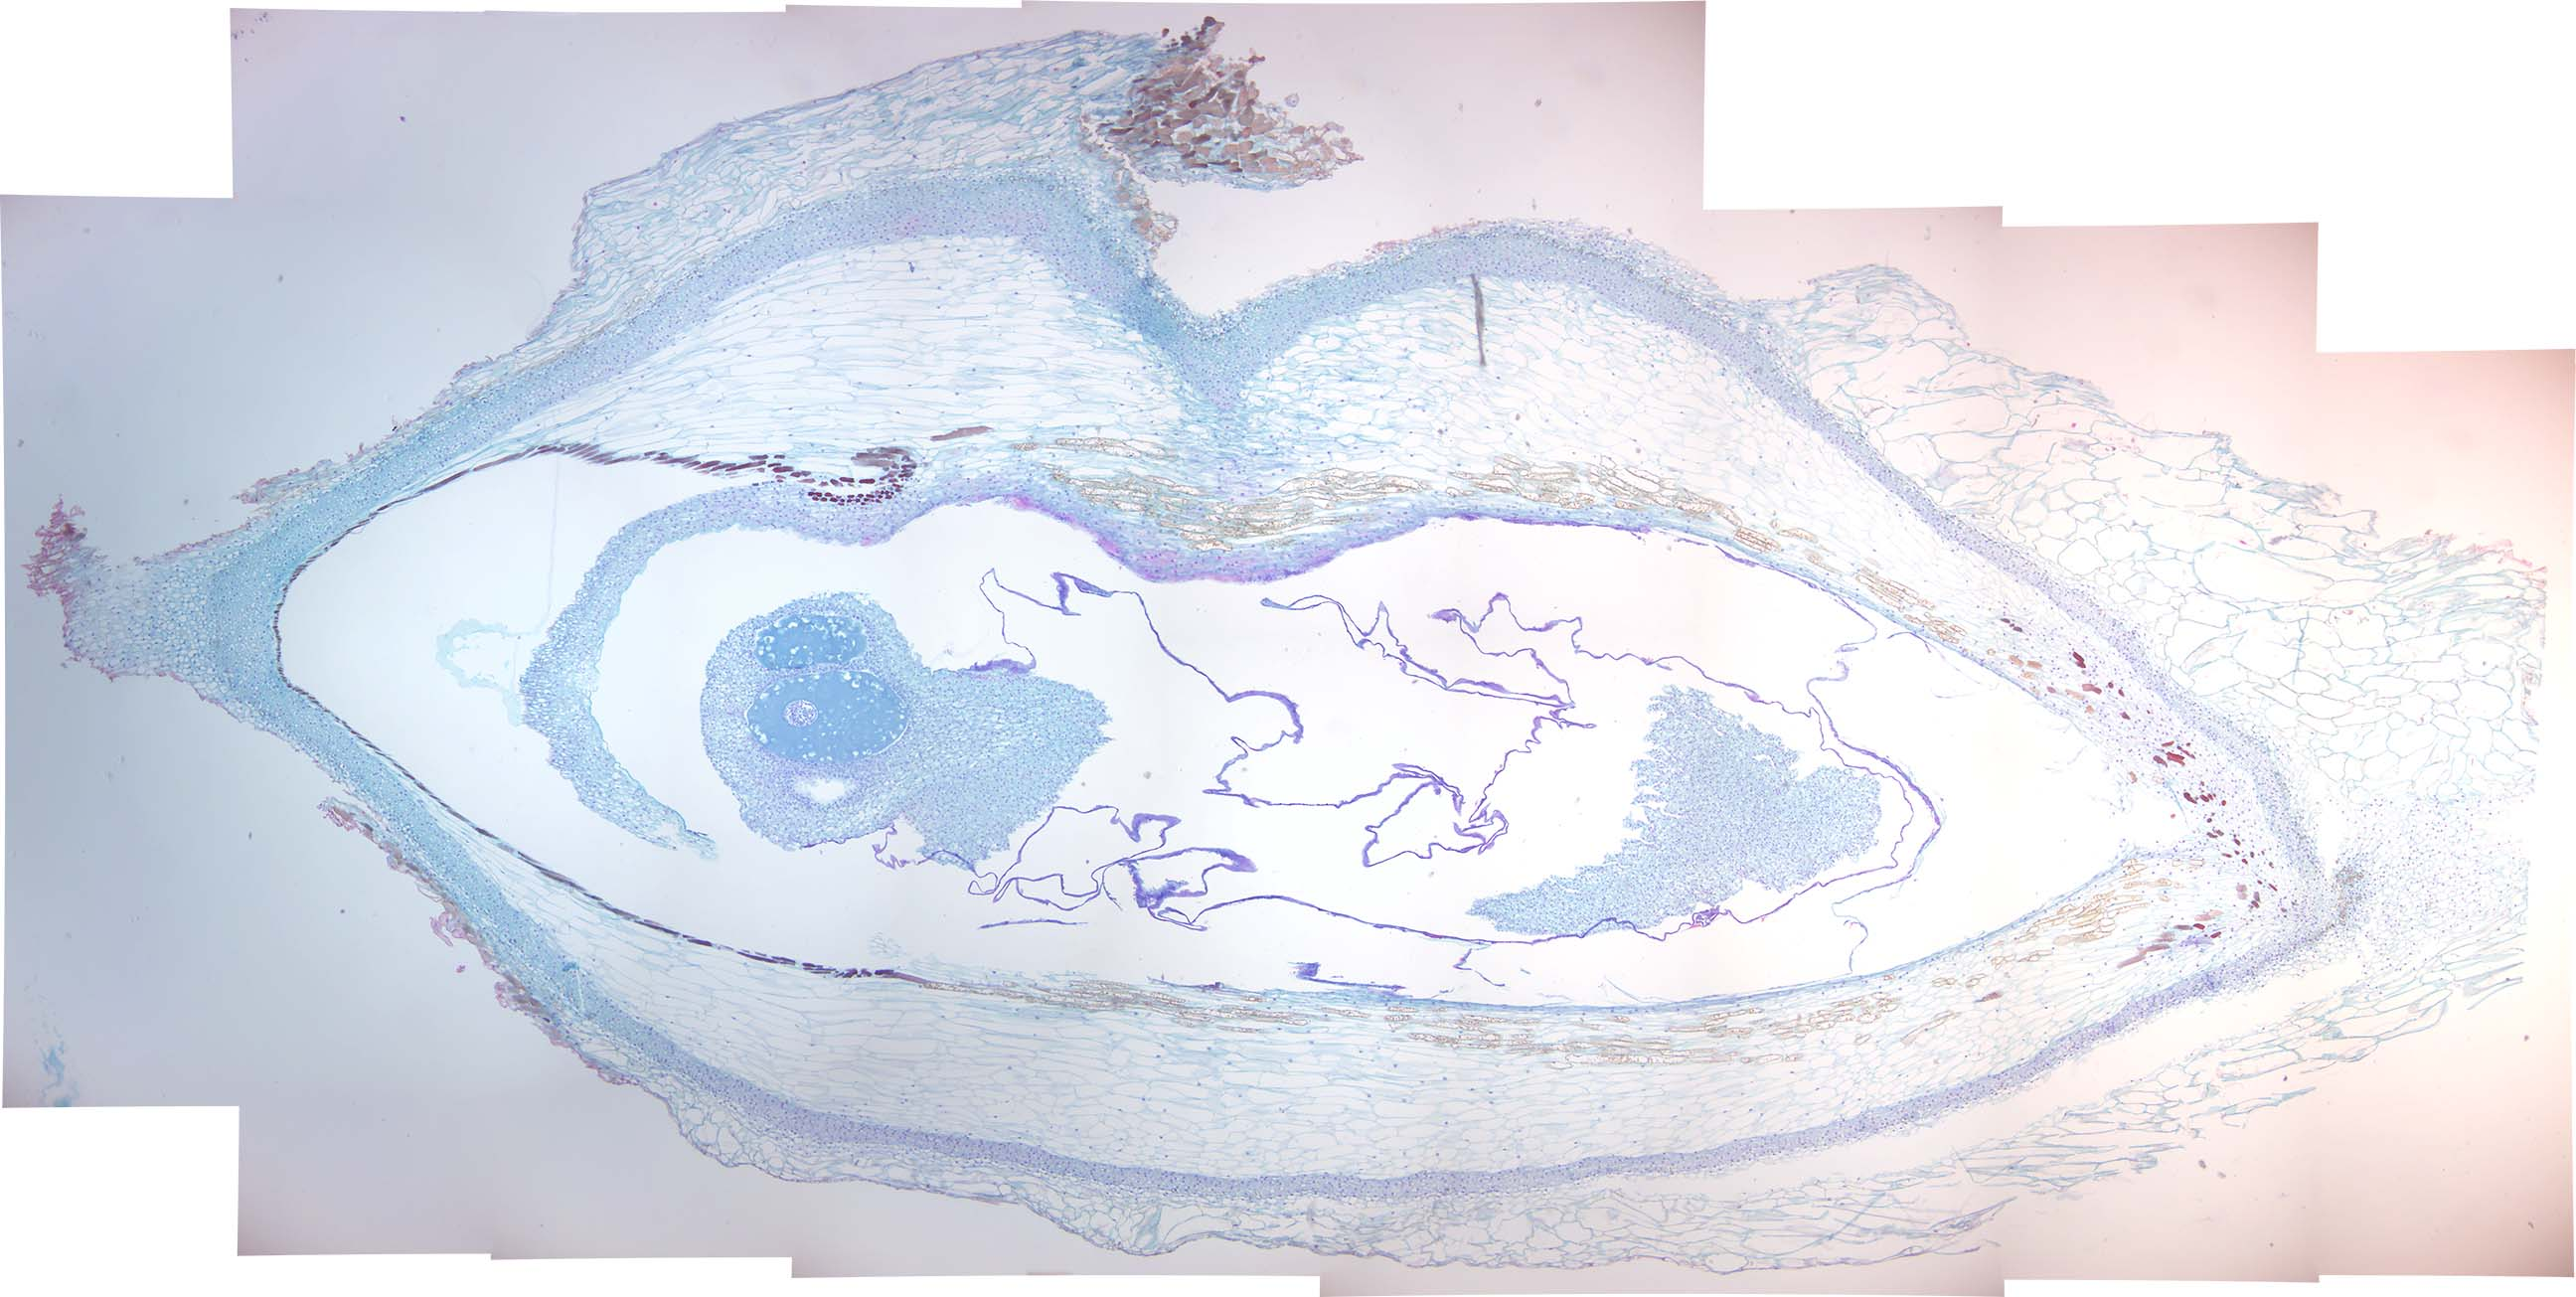
\includegraphics[width=0.7\linewidth]{./figures/gymnosperms/pine_ovule}

}

\caption{Pine ovule}\label{fig:pine}
\end{figure}

\begin{figure}

{\centering 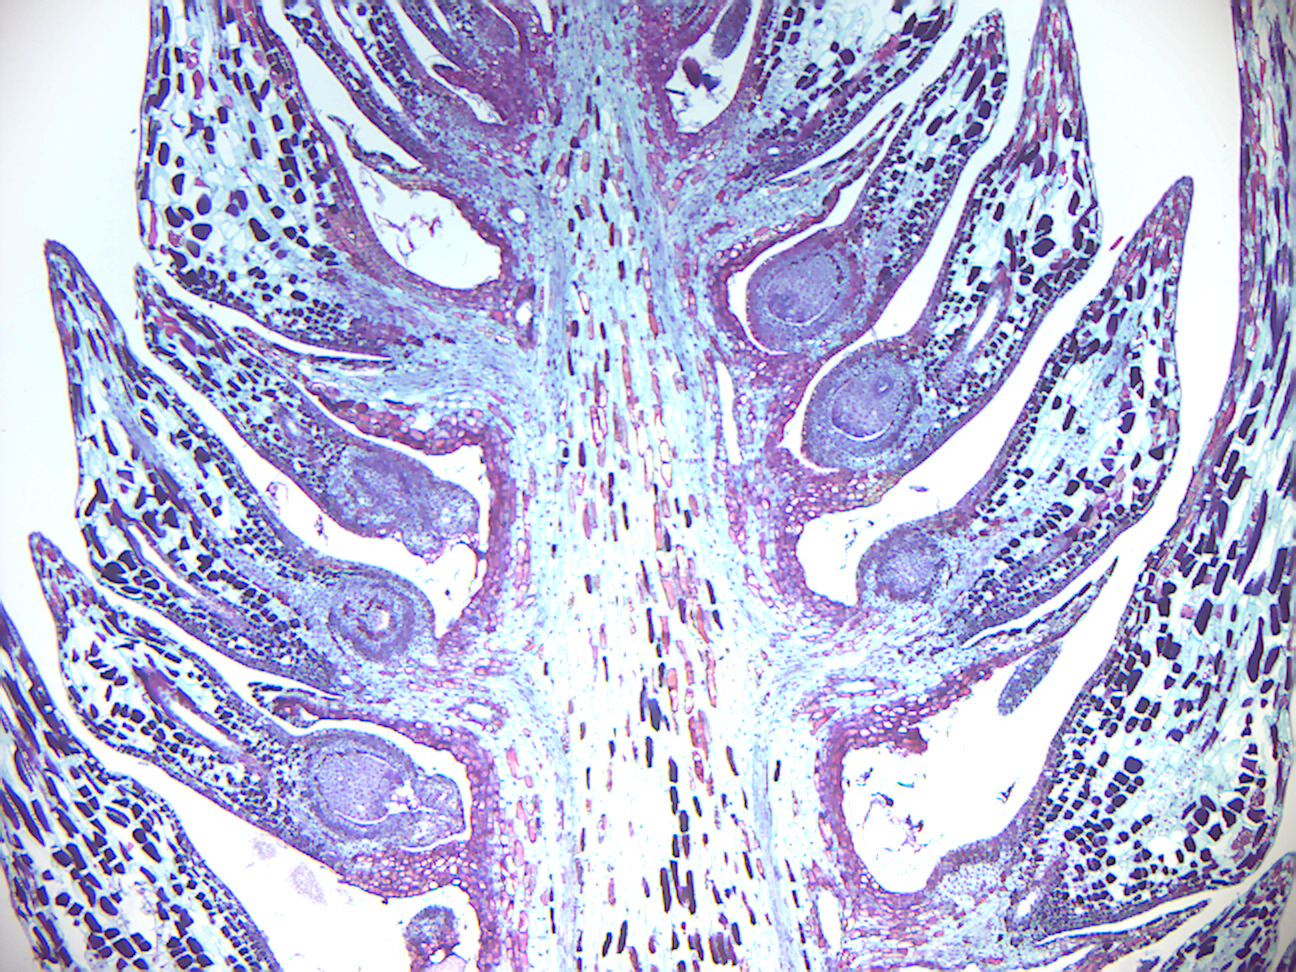
\includegraphics[width=0.7\linewidth]{./figures/gymnosperms/pine_ovulate}

}

\caption{Pine young ovulate cone.}\label{fig:ovulate}
\end{figure}

\begin{figure}

{\centering 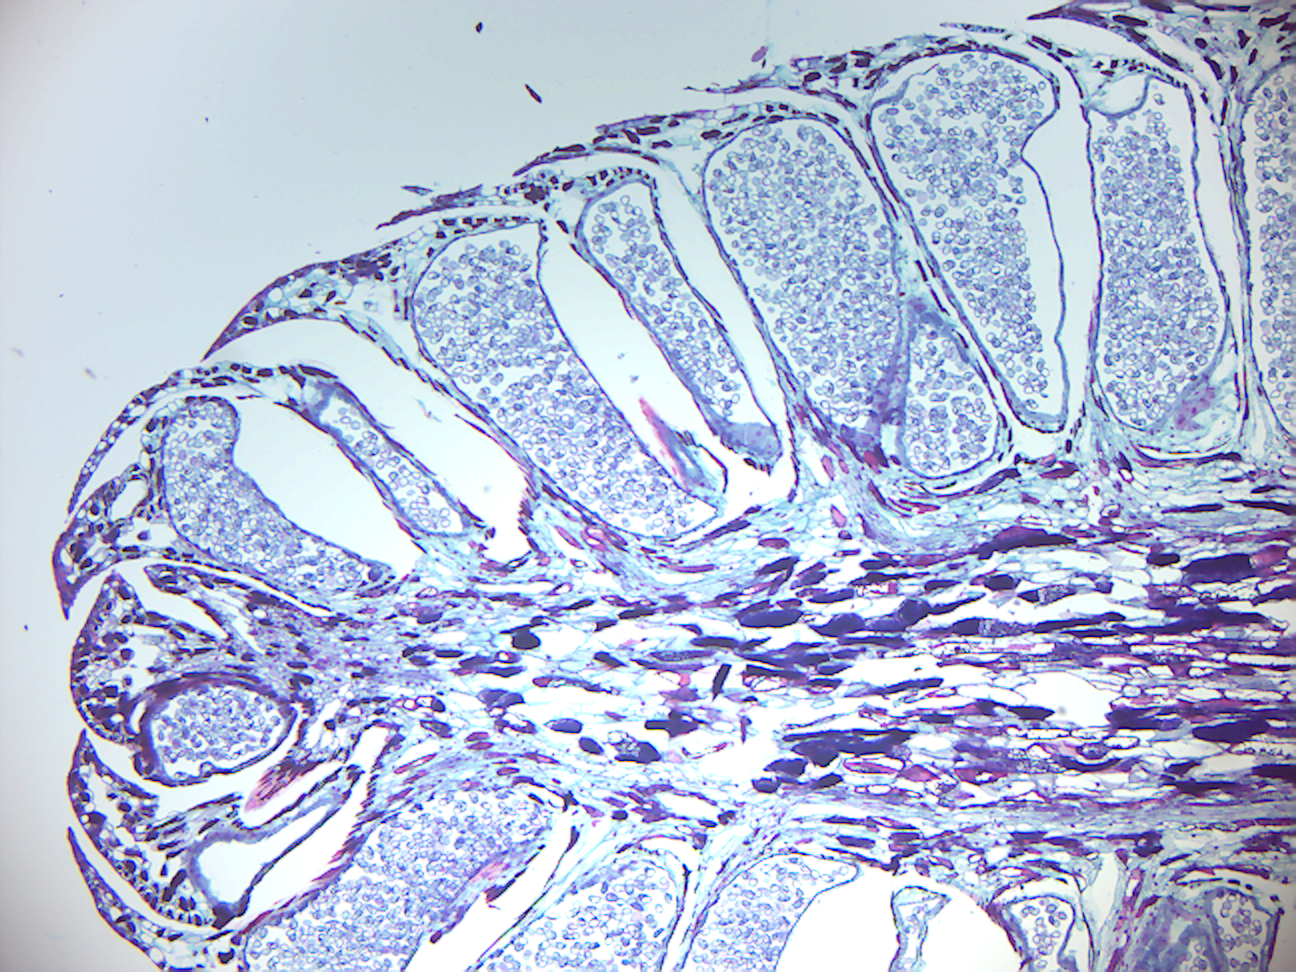
\includegraphics[width=0.7\linewidth]{./figures/gymnosperms/pine_staminate}

}

\caption{Pine staminate cone.}\label{fig:staminate}
\end{figure}

\begin{figure}

{\centering 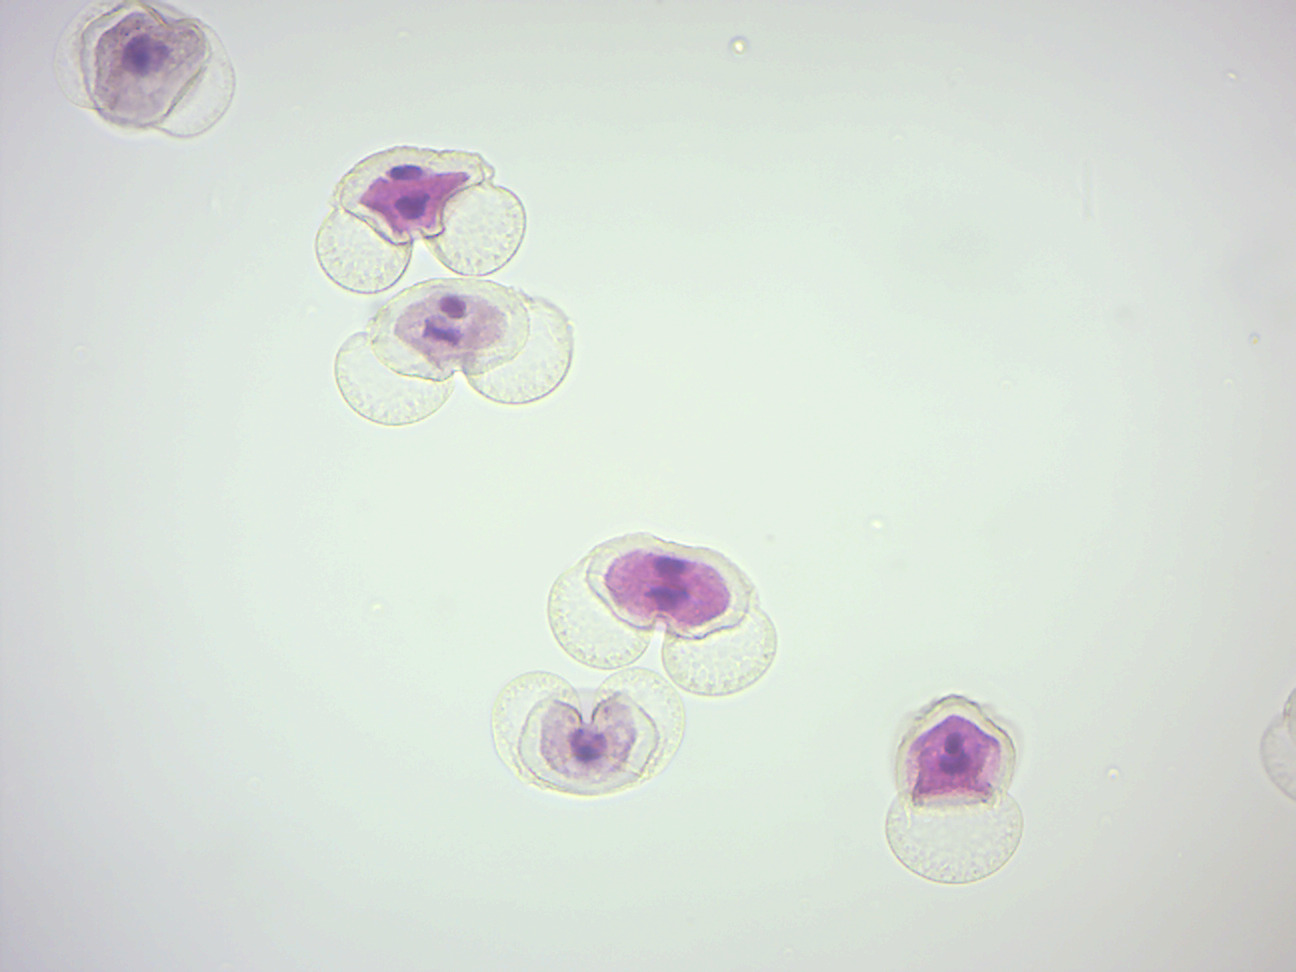
\includegraphics[width=0.7\linewidth]{./figures/gymnosperms/pine_pollen}

}

\caption{Pine pollen.}\label{fig:pollen}
\end{figure}

\begin{figure}

{\centering 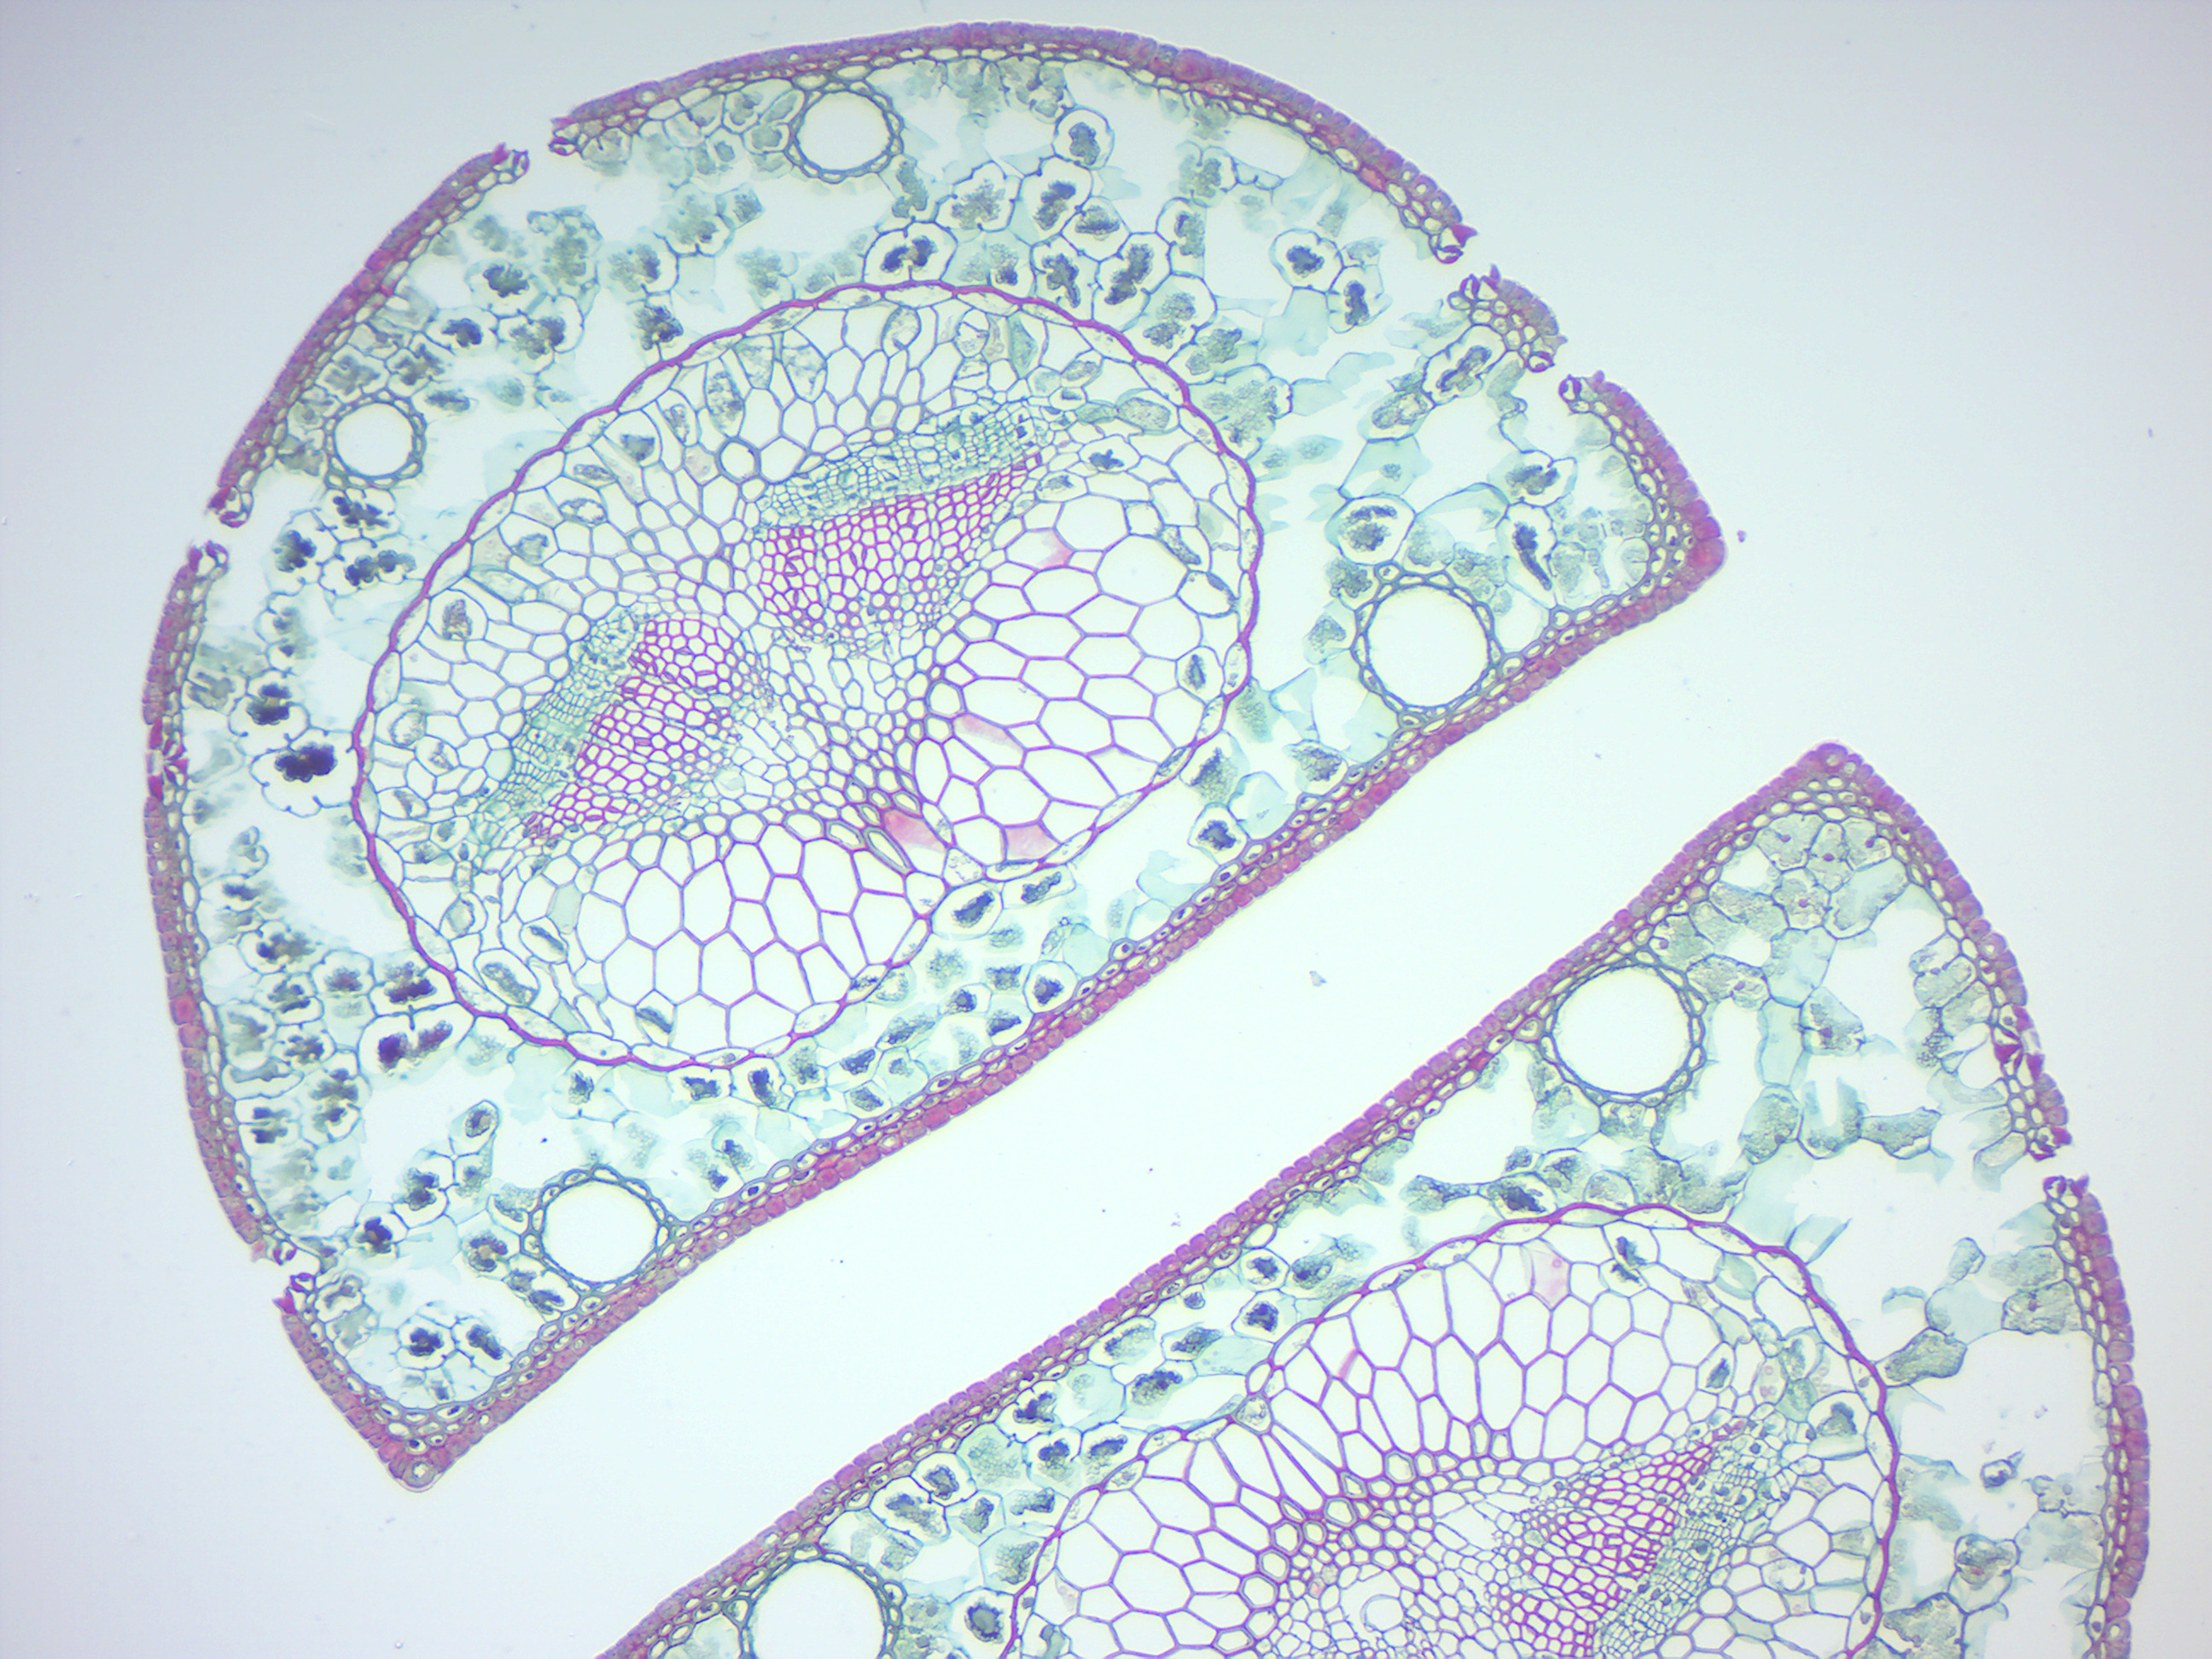
\includegraphics[width=0.7\linewidth]{./figures/gymnosperms/pine_needle}

}

\caption{Pine needle.}\label{fig:needle}
\end{figure}

\section{Angiosperms}\label{angiosperms}

The flowering plants, also known as angiosperms, Angiospermae or
Magnoliophyta, are the most diverse group of land plants, with 416
families, approximately 13,164 known genera and c. 295,383 known
species. Like gymnosperms, angiosperms are seed-producing plants.
However, they are distinguished from gymnosperms by characteristics
including flowers, endosperm within the seeds, and the production of
fruits that contain the seeds. Etymologically, angiosperm means a plant
that produces seeds within an enclosure; in other words, a fruiting
plant. The term comes from the Greek words angeion (``case'' or
``casing'') and sperma (``seed''). The ancestors of flowering plants
diverged from gymnosperms in the Triassic Period, 245 to 202 million
years ago (mya), and the first flowering plants are known from 160 mya.
They diversified extensively during the Lower Cretaceous, became
widespread by 120 mya, and replaced conifers as the dominant trees from
100 to 60 mya.

The characteristic feature of angiosperms is the flower. Flowers show
remarkable variation in form and elaboration, and provide the most
trustworthy external characteristics for establishing relationships
among angiosperm species. The function of the flower is to ensure
fertilization of the ovule and development of fruit containing seeds.
The floral apparatus may arise terminally on a shoot or from the axil of
a leaf (where the petiole attaches to the stem). Occasionally, as in
violets, a flower arises singly in the axil of an ordinary foliage-leaf.
More typically, the flower-bearing portion of the plant is sharply
distinguished from the foliage-bearing or vegetative portion, and forms
a more or less elaborate branch-system called an inflorescence.

\begin{figure}

{\centering 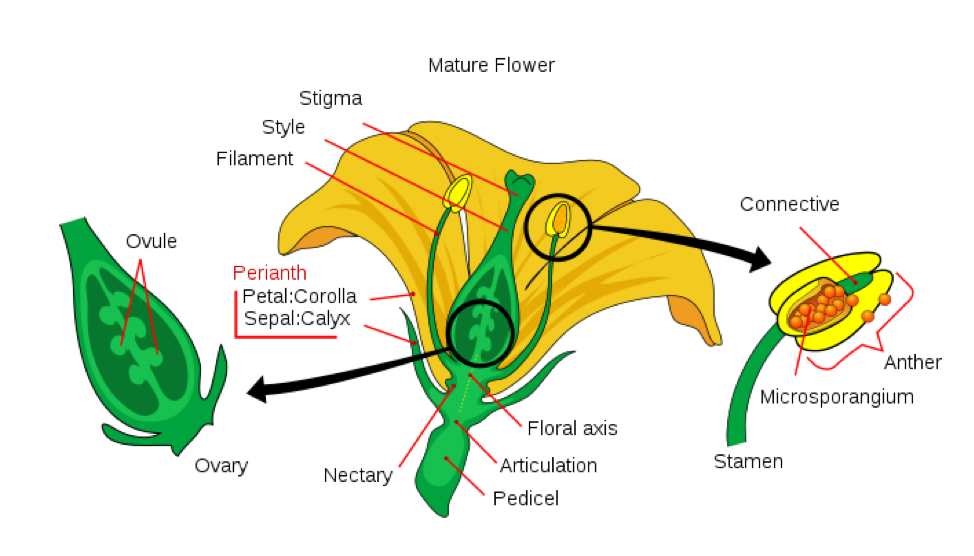
\includegraphics[width=0.7\linewidth]{./figures/gymnosperms/mature_flower}

}

\caption{\href{https://commons.wikimedia.org/wiki/File:Mature_flower_diagram.svg}{Anatomy
of the flower.}}\label{fig:flower}
\end{figure}

There are two kinds of reproductive cells produced by flowers.
Microspores, which will divide to become pollen grains, are the ``male''
cells and are borne in the stamens (or microsporophylls). The ``female''
cells called megaspores, which will divide to become the egg cell
(megagametogenesis), are contained in the ovule and enclosed in the
carpel (or megasporophyll).

The flower may consist only of these parts, as in willow, where each
flower comprises only a few stamens or two carpels. Usually, other
structures are present and serve to protect the sporophylls and to form
an envelope attractive to pollinators. The individual members of these
surrounding structures are known as sepals and petals (or tepals in
flowers such as \emph{Lilium} where sepals and petals are not distinguishable
from each other). The outer series (calyx of sepals) is usually green
and leaf-like, and functions to protect the rest of the flower,
especially the bud. The inner series (corolla of petals) is, in general,
white or brightly colored, and is more delicate in structure. It
functions to attract insect or bird pollinators. Attraction is effected
by color, scent, and nectar, which may be secreted in some part of the
flower. The characteristics that attract pollinators account for the
popularity of flowers and flowering plants among humans.

While the majority of flowers are perfect or hermaphrodite (having both
pollen and ovule producing parts in the same flower structure),
flowering plants have developed numerous morphological and physiological
mechanisms to reduce or prevent self-fertilization. Heteromorphic
flowers have short carpels and long stamens, or vice versa, so animal
pollinators cannot easily transfer pollen to the pistil (receptive part
of the carpel). Homomorphic flowers may employ a biochemical
(physiological) mechanism called self-incompatibility to discriminate
between self and non-self pollen grains. In other species, the male and
female parts are morphologically separated, developing on different
flowers.

\subsection{Sexual Reproduction}\label{sexual-reproduction}

Double fertilization refers to a process in which two sperm cells
fertilize cells in the ovary. This process begins when a pollen grain
adheres to the stigma of the pistil (female reproductive structure),
germinates, and grows a long pollen tube. While this pollen tube is
growing, a haploid generative cell travels down the tube behind the tube
nucleus. The generative cell divides by mitosis to produce two haploid
(n) sperm cells. As the pollen tube grows, it makes its way from the
stigma, down the style and into the ovary. Here the pollen tube reaches
the micropyle of the ovule and digests its way into one of the
synergids, releasing its contents (which include the sperm cells). The
synergid that the cells were released into degenerates and one sperm
makes its way to fertilize the egg cell, producing a diploid (2n)
zygote. The second sperm cell fuses with both central cell nuclei,
producing a triploid (3n) cell. As the zygote develops into an embryo,
the triploid cell develops into the endosperm, which serves as the
embryo's food supply. The ovary will now develop into a fruit and the
ovule will develop into a seed.

As the development of embryo and endosperm proceeds within the embryo
sac, the sac wall enlarges and combines with the nucellus (which is
likewise enlarging) and the integument to form the seed coat. The ovary
wall develops to form the fruit or pericarp, whose form is closely
associated with type of seed dispersal system.

Frequently, the influence of fertilization is felt beyond the ovary, and
other parts of the flower take part in the formation of the fruit, e.g.,
the floral receptacle in the apple, strawberry, and others.

The character of the seed coat bears a definite relation to that of the
fruit. They protect the embryo and aid in dissemination; they may also
directly promote germination. Among plants with indehiscent fruits, in
general, the fruit provides protection for the embryo and secures
dissemination. In this case, the seed coat is only slightly developed.
If the fruit is dehiscent and the seed is exposed, in general, the
seed-coat is well developed, and must discharge the functions otherwise
executed by the fruit.

Flowering plants generate gametes using meiosis. Meiosis takes place in the ovule (a structure within the
ovary that is located within the pistil at the center of the flower). A
diploid cell (megaspore mother cell) in the ovule undergoes meiosis
(involving two successive cell divisions) to produce four cells
(megaspores or female gametes) with haploid nuclei. One of these four
cells (megaspore) then undergoes three successive mitotic divisions to
produce an immature embryo sac (megagametocyte) with eight haploid
nuclei. Next, these nuclei are segregated into separate cells by
cytokinesis to producing 3 antipodal cells, 2 synergid cells and an egg
cell. Two polar nuclei are left in the central cell of the embryo sac.

Pollen is also produced by meiosis in the male anther (microsporangium).
During meiosis, a diploid microspore mother cell undergoes two
successive meiotic divisions to produce 4 haploid cells (microspores or
male gametes). Each of these microspores, after further mitoses, becomes
a pollen grain (microgametophyte) containing two haploid generative
(sperm) cells and a tube nucleus. When a pollen grain makes contact with
the female stigma, the pollen grain forms a pollen tube that grows down
the style into the ovary. In the act of fertilization, a male sperm
nucleus fuses with the female egg nucleus to form a diploid zygote that
can then develop into an embryo within the newly forming seed. Upon
germination of the seed, a new plant can grow and mature.

\begin{figure}

{\centering 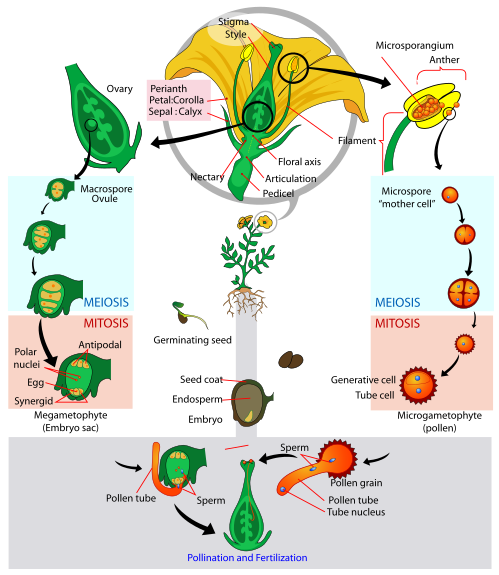
\includegraphics[width=0.7\linewidth]{./figures/gymnosperms/angiosperm_life_cycle}

}

\caption{\href{https://commons.wikimedia.org/wiki/File:Angiosperm_life_cycle_diagram-en.svg}{Life
cycle of angiosperms.}}\label{fig:angiosperm}
\end{figure}

\section{View Prepared Slides of
Angiosperms}\label{view-prepared-slides-of-angiosperms}

\begin{enumerate}
\def\labelenumi{\arabic{enumi}.}
\tightlist
\item
  Lily anther (Figure \ref{fig:lilianther})

  \begin{itemize}
  \tightlist
  \item
    Identify: anther, microsporangium, pollen grains with tube and
    generative nuclei. The structure in the middle of the slide is the
    Lily ovary. The anthers are around the ovary.
  \end{itemize}
\item
  Lily anther with mature pollen (Figure \ref{fig:lilipollen})

  \begin{itemize}
  \tightlist
  \item
    Identify: pollen grain, tube cell with nucleus, generative cell with
    nucleus
  \end{itemize}
\item
  Lily pollen tubes (Figure \ref{fig:lilitubes})

  \begin{itemize}
  \tightlist
  \item
    Identify: sigma tissue, pollen tubes
  \end{itemize}
\item
  Lily ovary (Figure \ref{fig:liliovary})

  \begin{itemize}
  \tightlist
  \item
    Identify: ovary, ovules, female gametophytes (embryo sac). If this
    slides is not available, you can observe the lily ovary in the
    ``Lily anther x.s.'' slide.
  \end{itemize}
\item
  \emph{Tilia} 2 year old stem (Figure \ref{fig:tilia})
\item
  \emph{Capsella} seeds (Figure \ref{fig:capsella})

  \begin{itemize}
  \tightlist
  \item
    Identify: embryo, cotyledons, root tip, shoot tip
  \end{itemize}
\end{enumerate}

\begin{figure}

{\centering 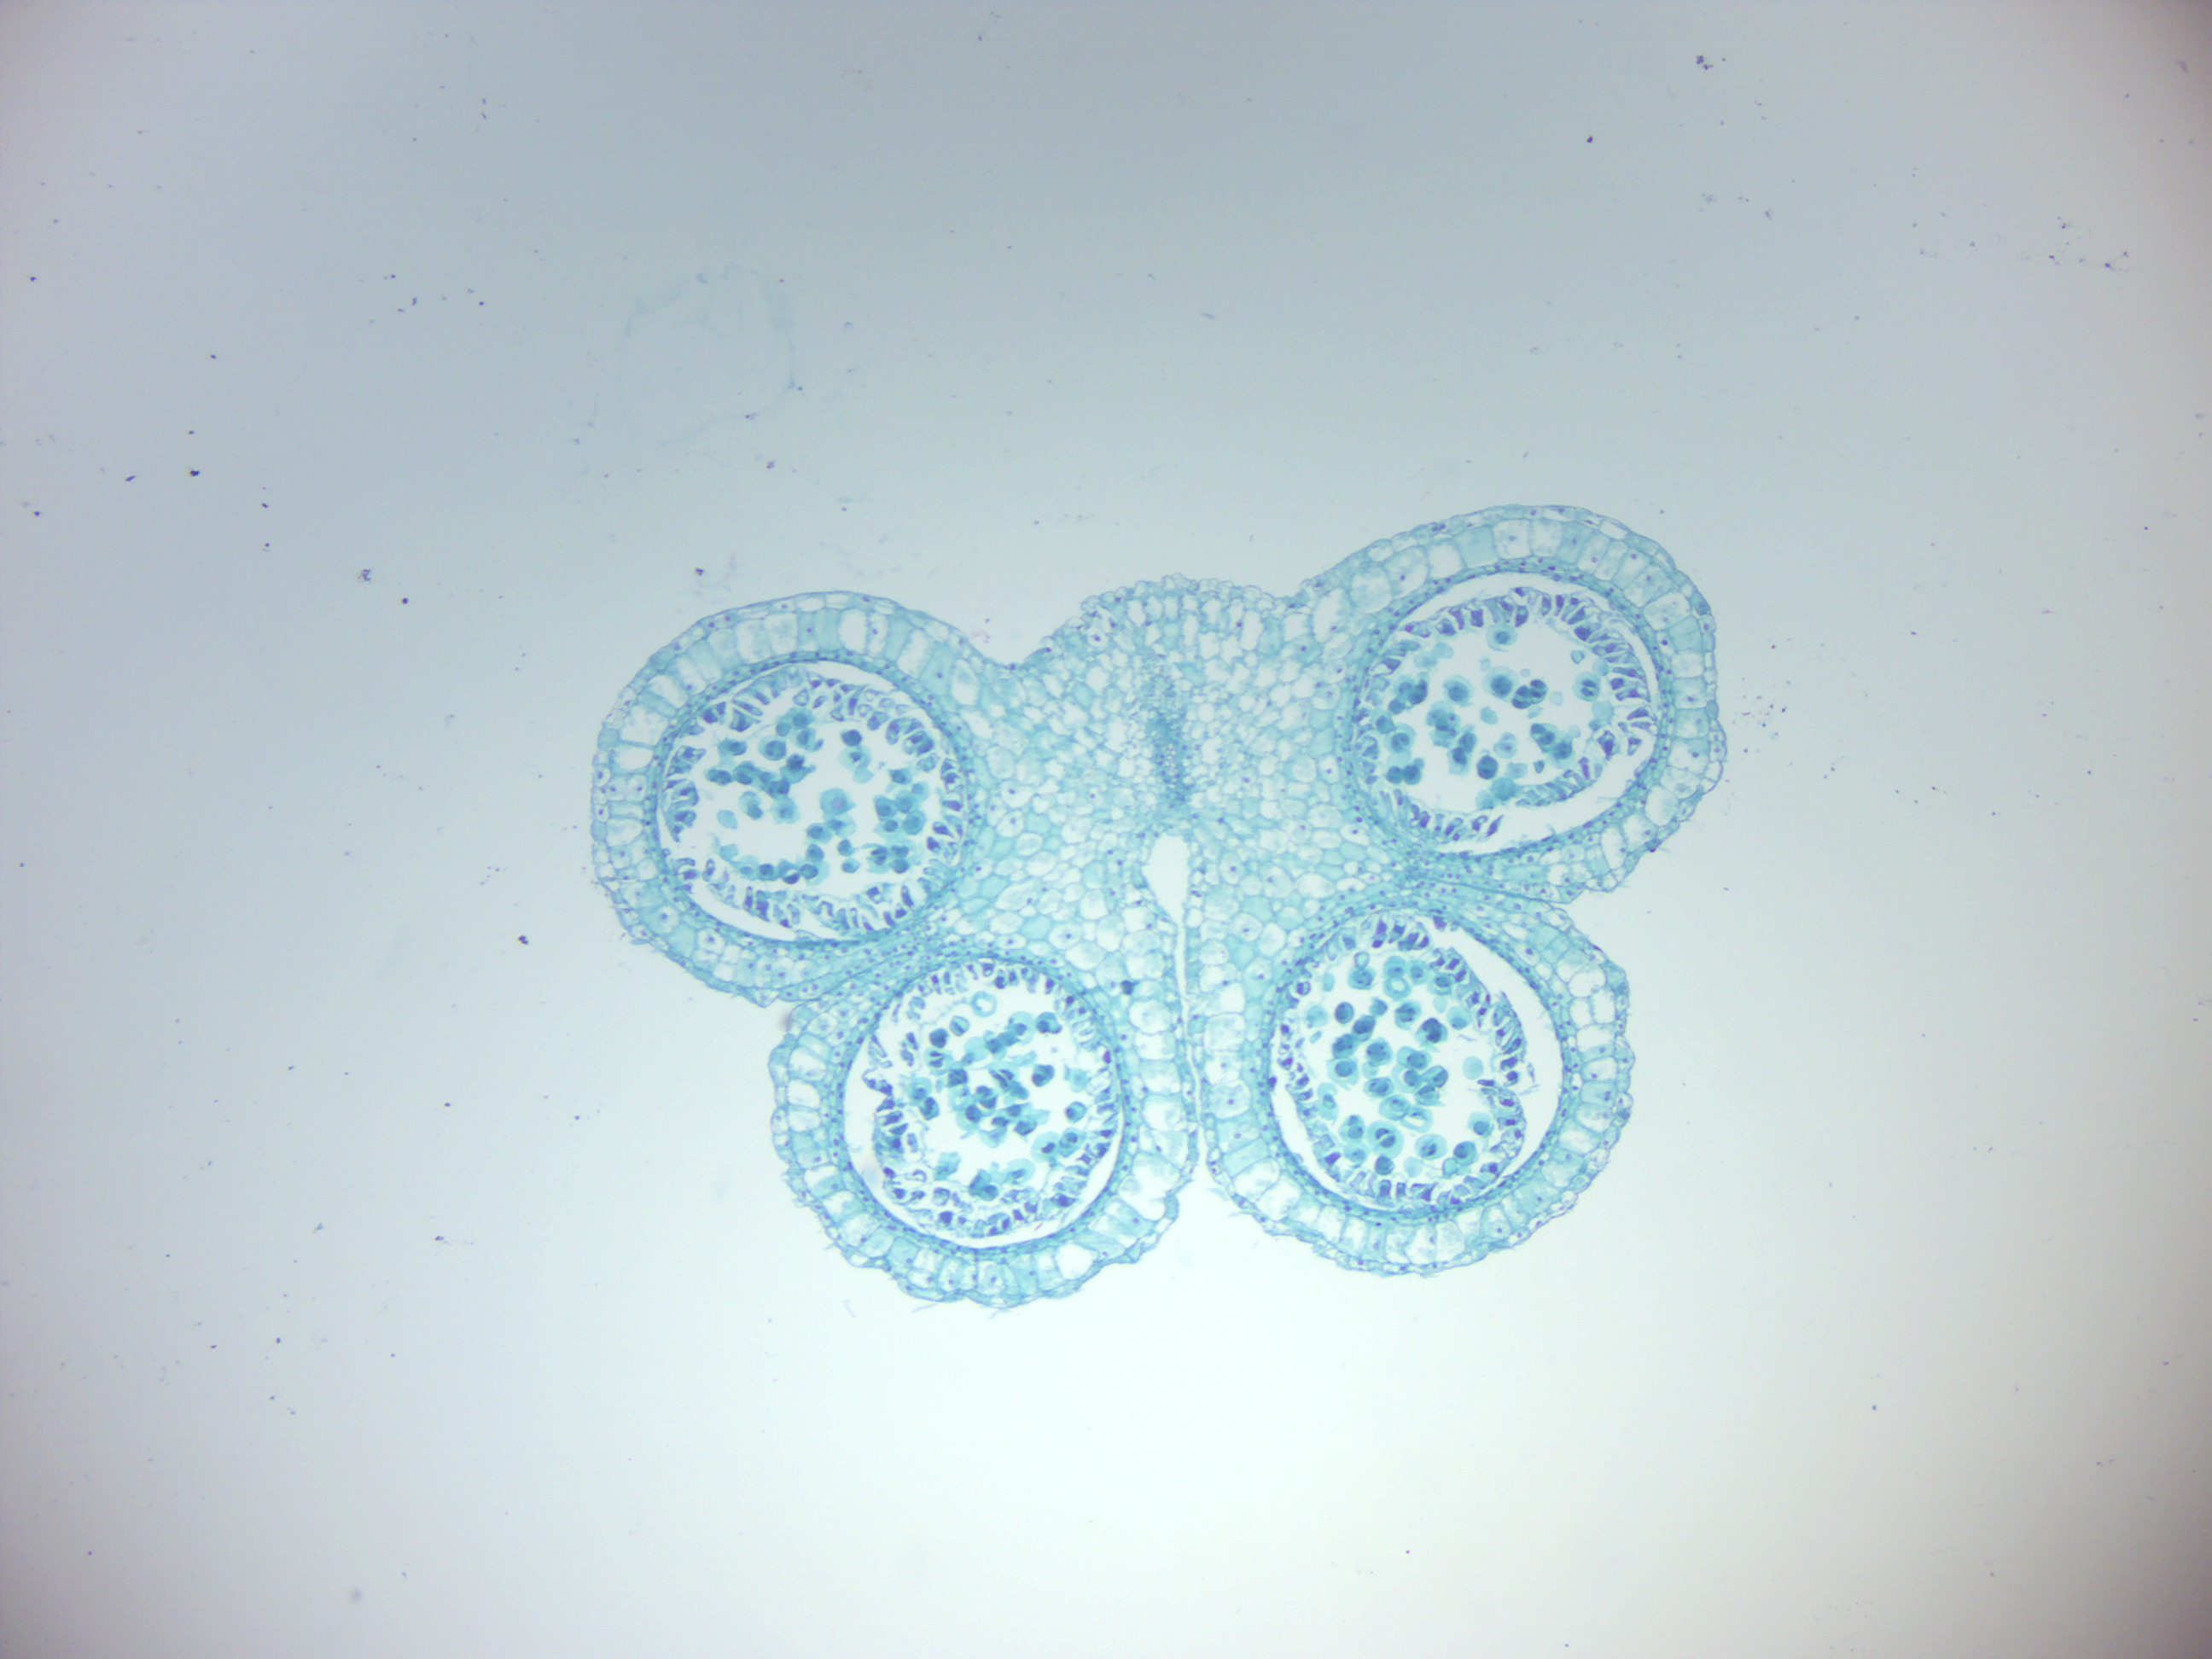
\includegraphics[width=0.7\linewidth]{./figures/gymnosperms/lily_anther}

}

\caption{Lily anther.}\label{fig:lilianther}
\end{figure}

\begin{figure}

{\centering 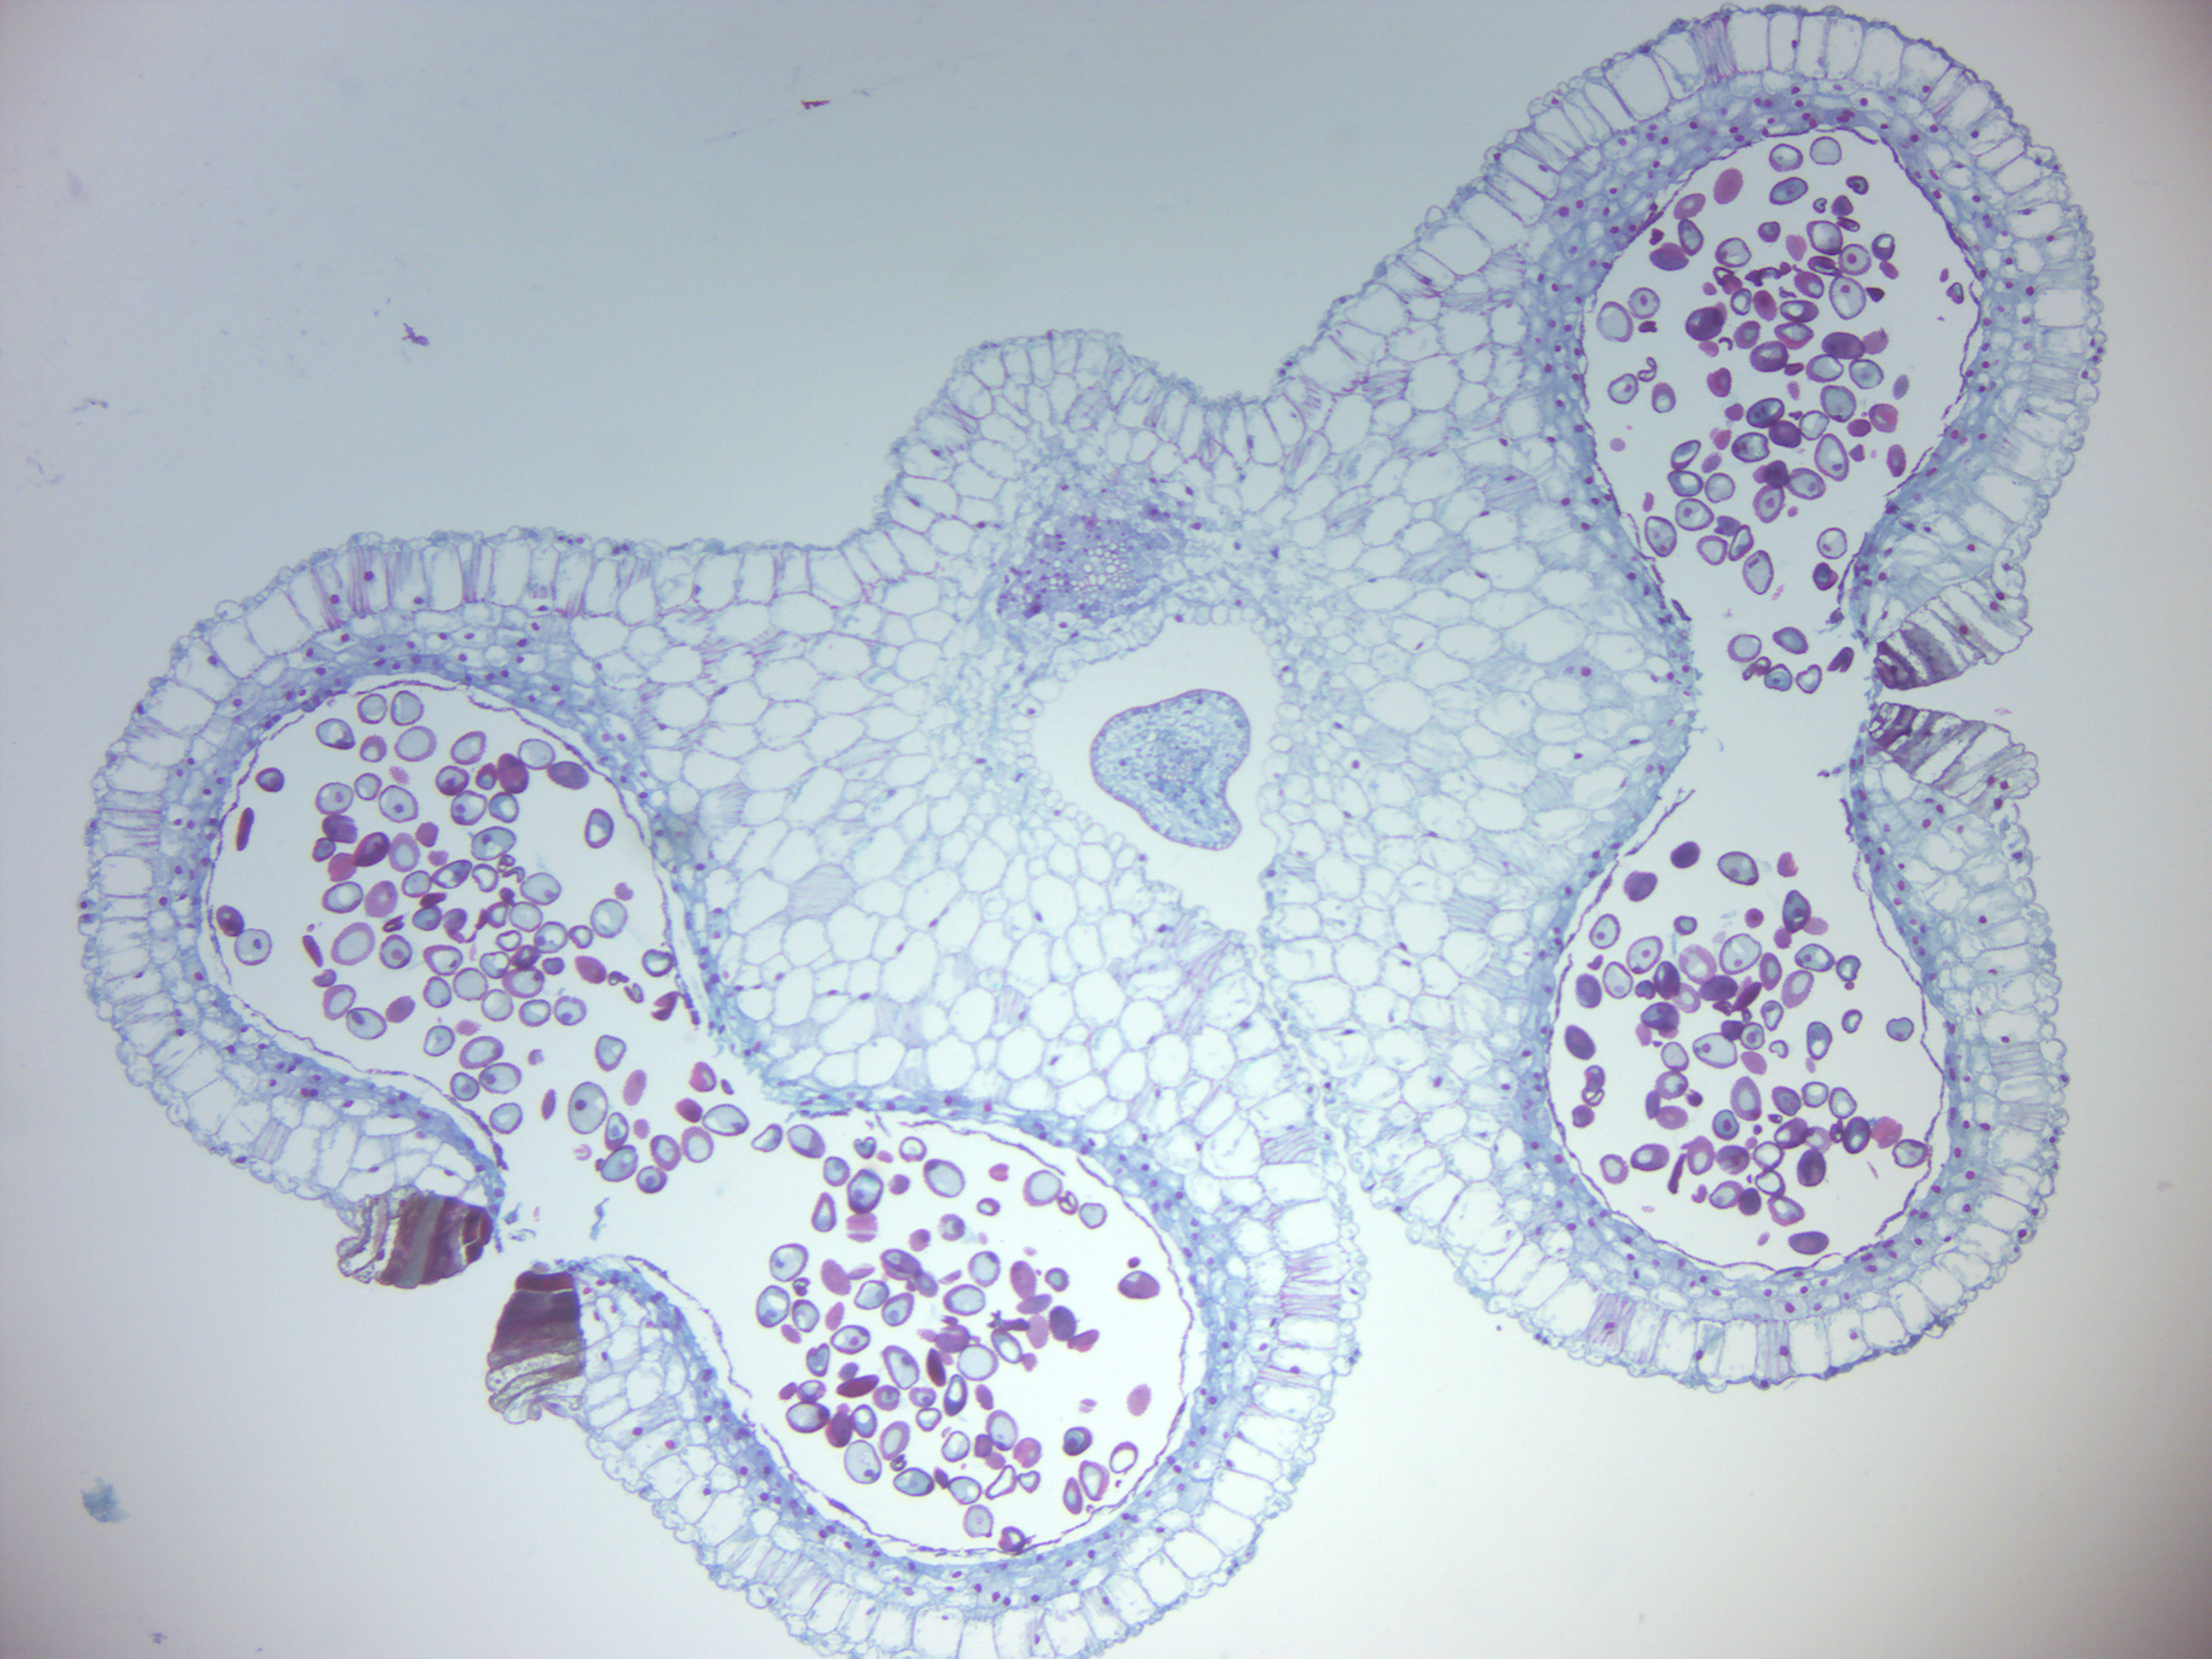
\includegraphics[width=0.7\linewidth]{./figures/gymnosperms/lily_pollen}

}

\caption{Lily anther with mature pollen.}\label{fig:lilipollen}
\end{figure}

\begin{figure}

{\centering 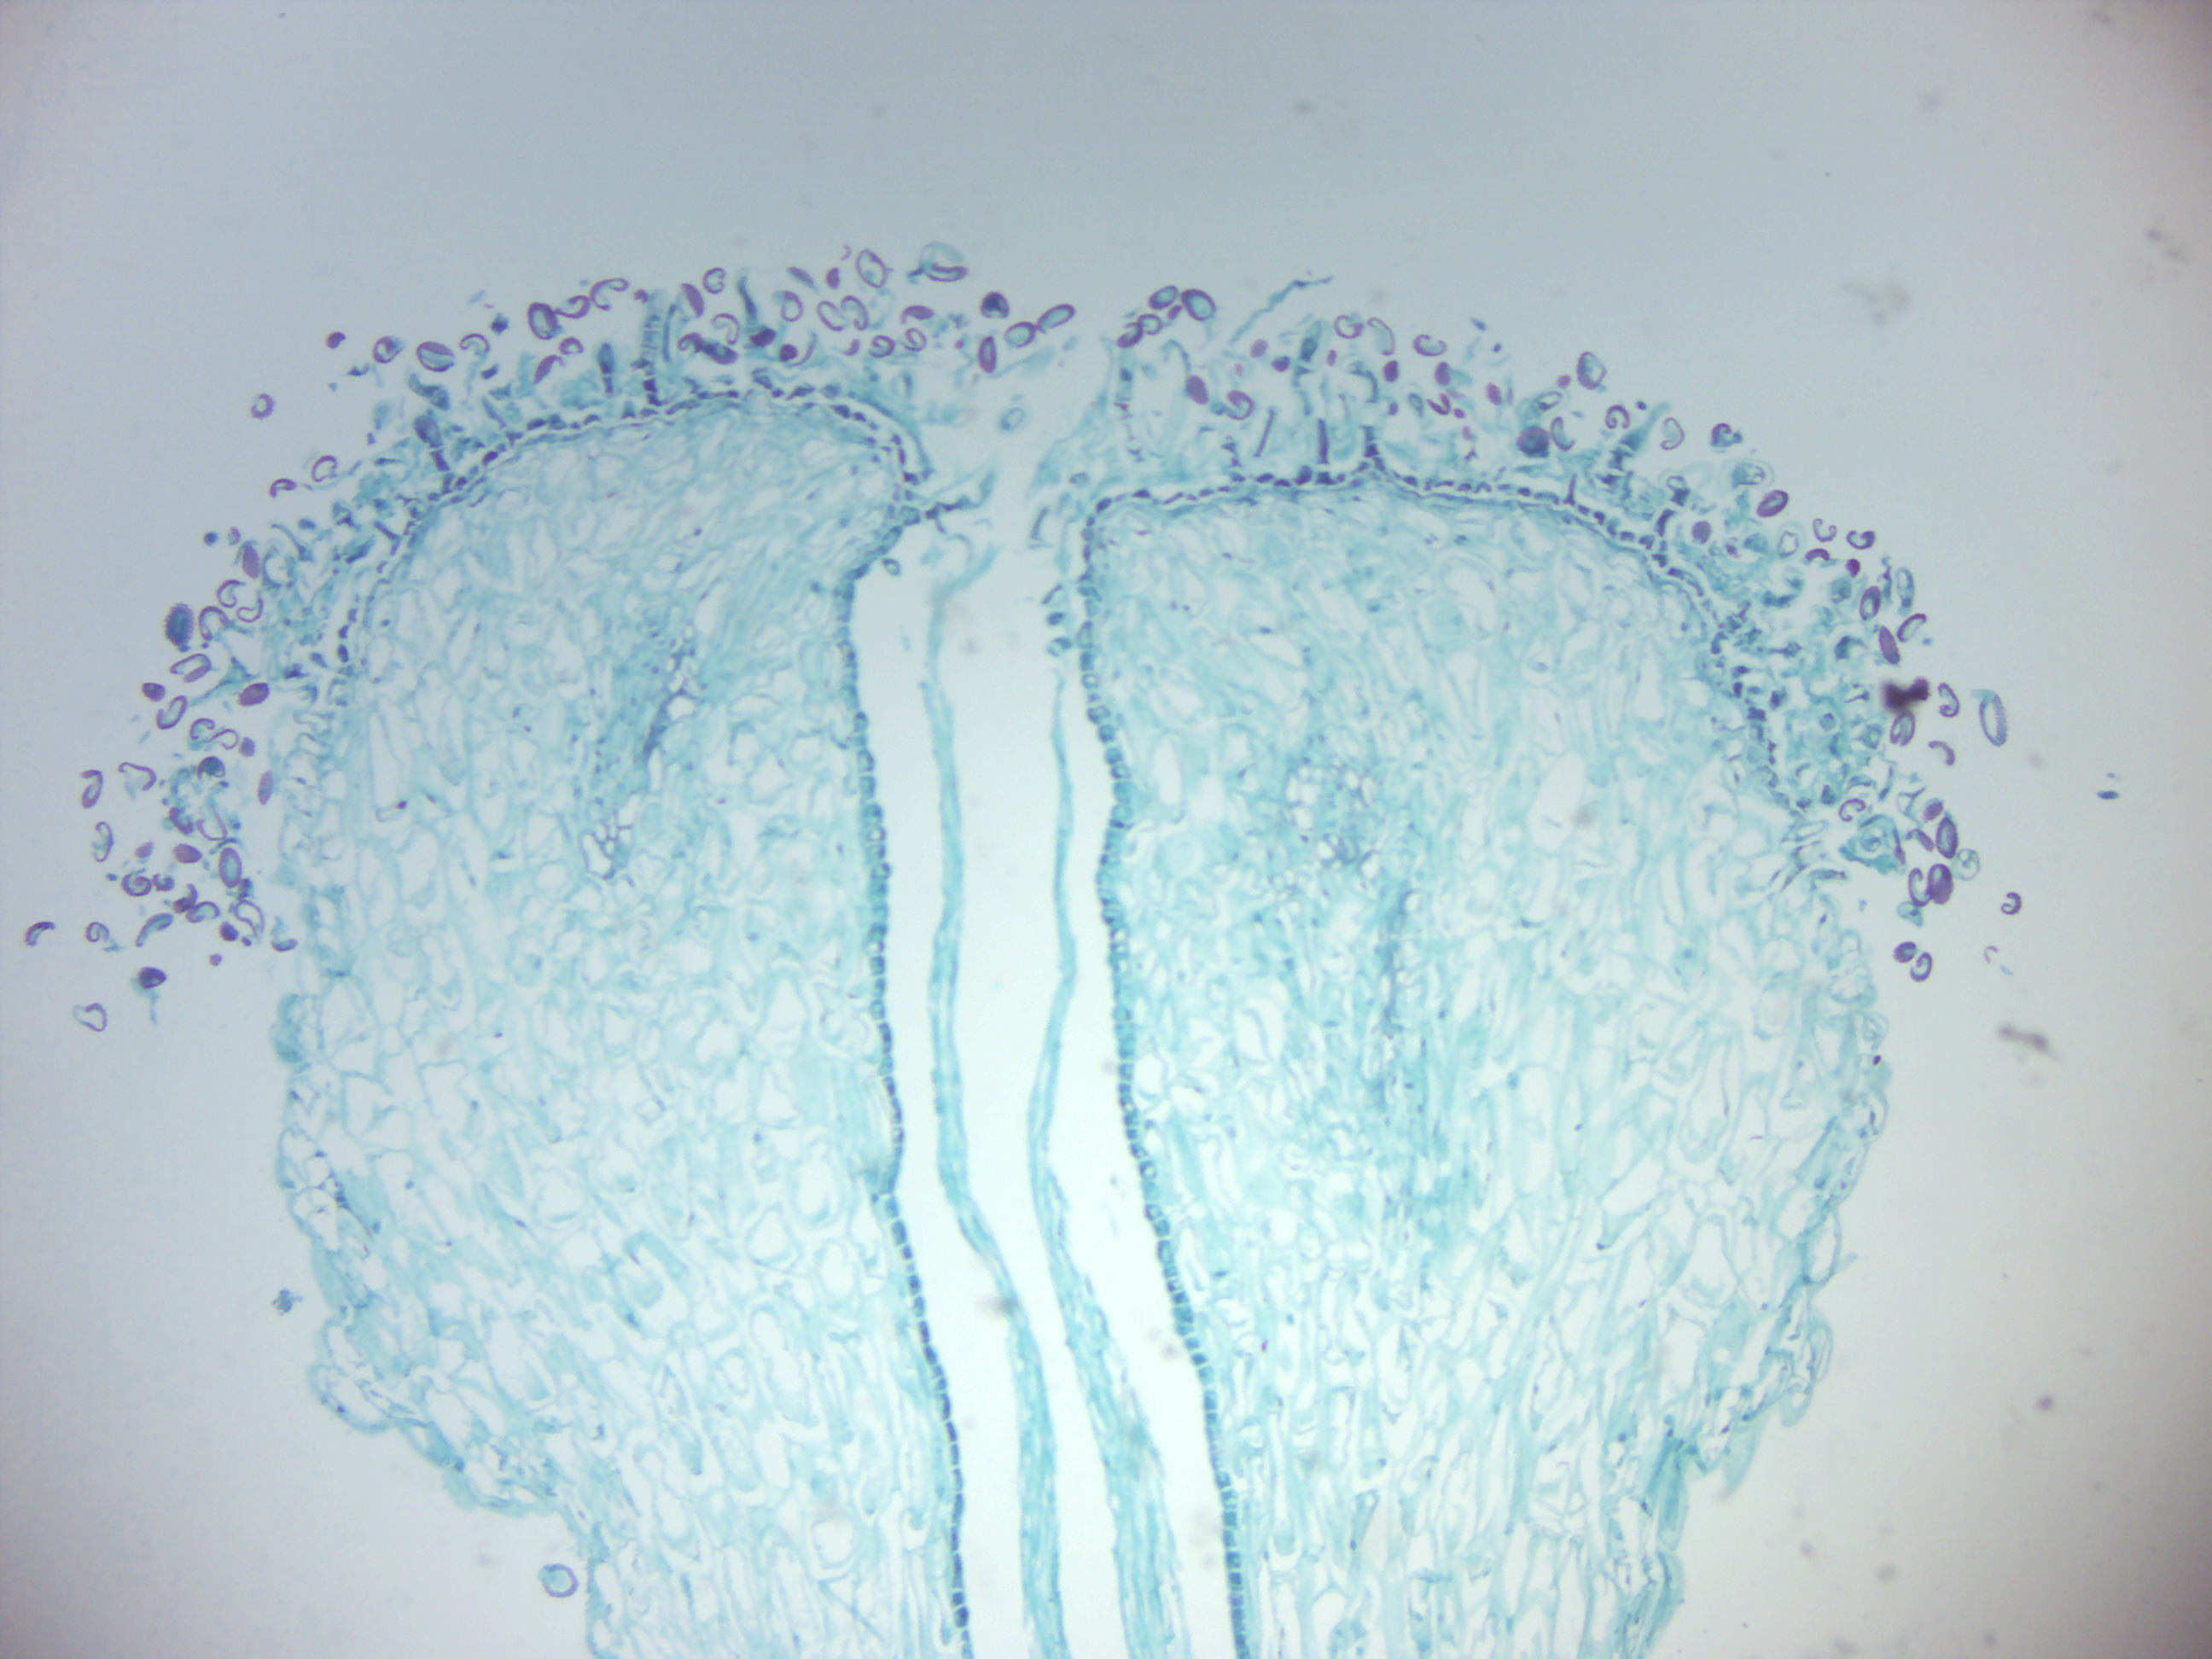
\includegraphics[width=0.7\linewidth]{./figures/gymnosperms/lily_tubes}

}

\caption{Lily pollen tubes.}\label{fig:lilitubes}
\end{figure}

\begin{figure}

{\centering 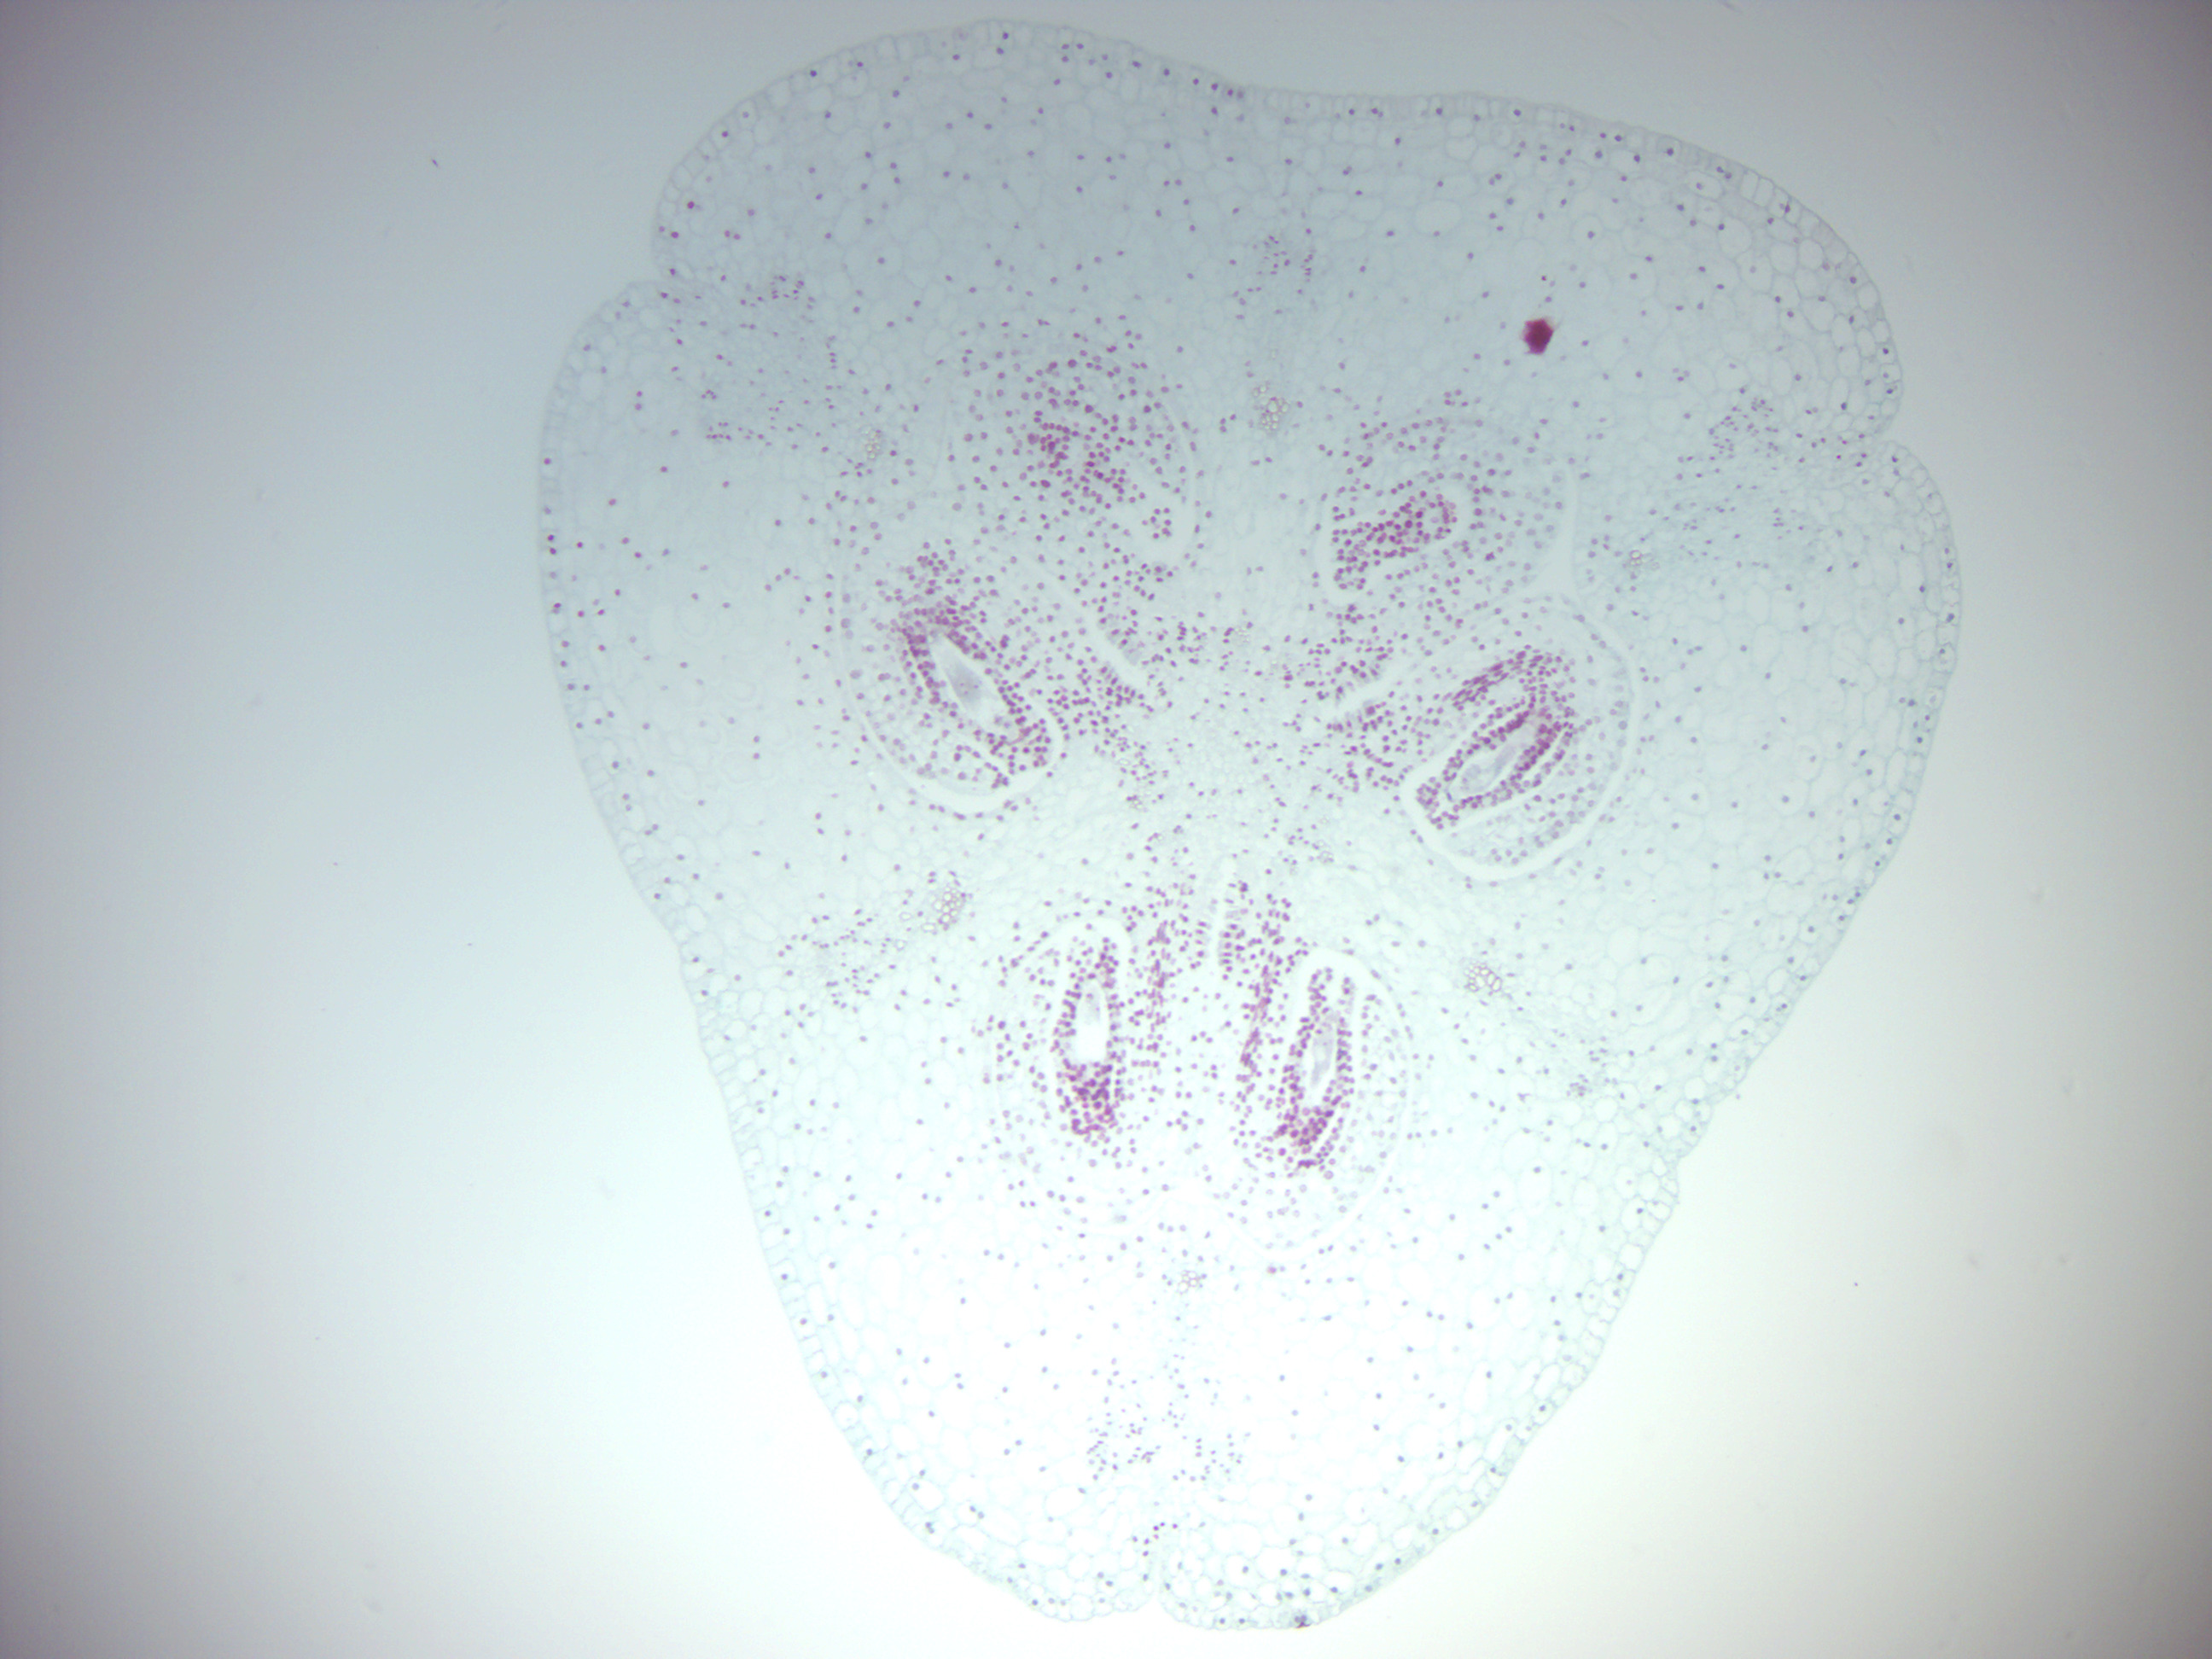
\includegraphics[width=0.7\linewidth]{./figures/gymnosperms/lily_ovary}

}

\caption{Lily ovary.}\label{fig:liliovary}
\end{figure}

\begin{figure}

{\centering 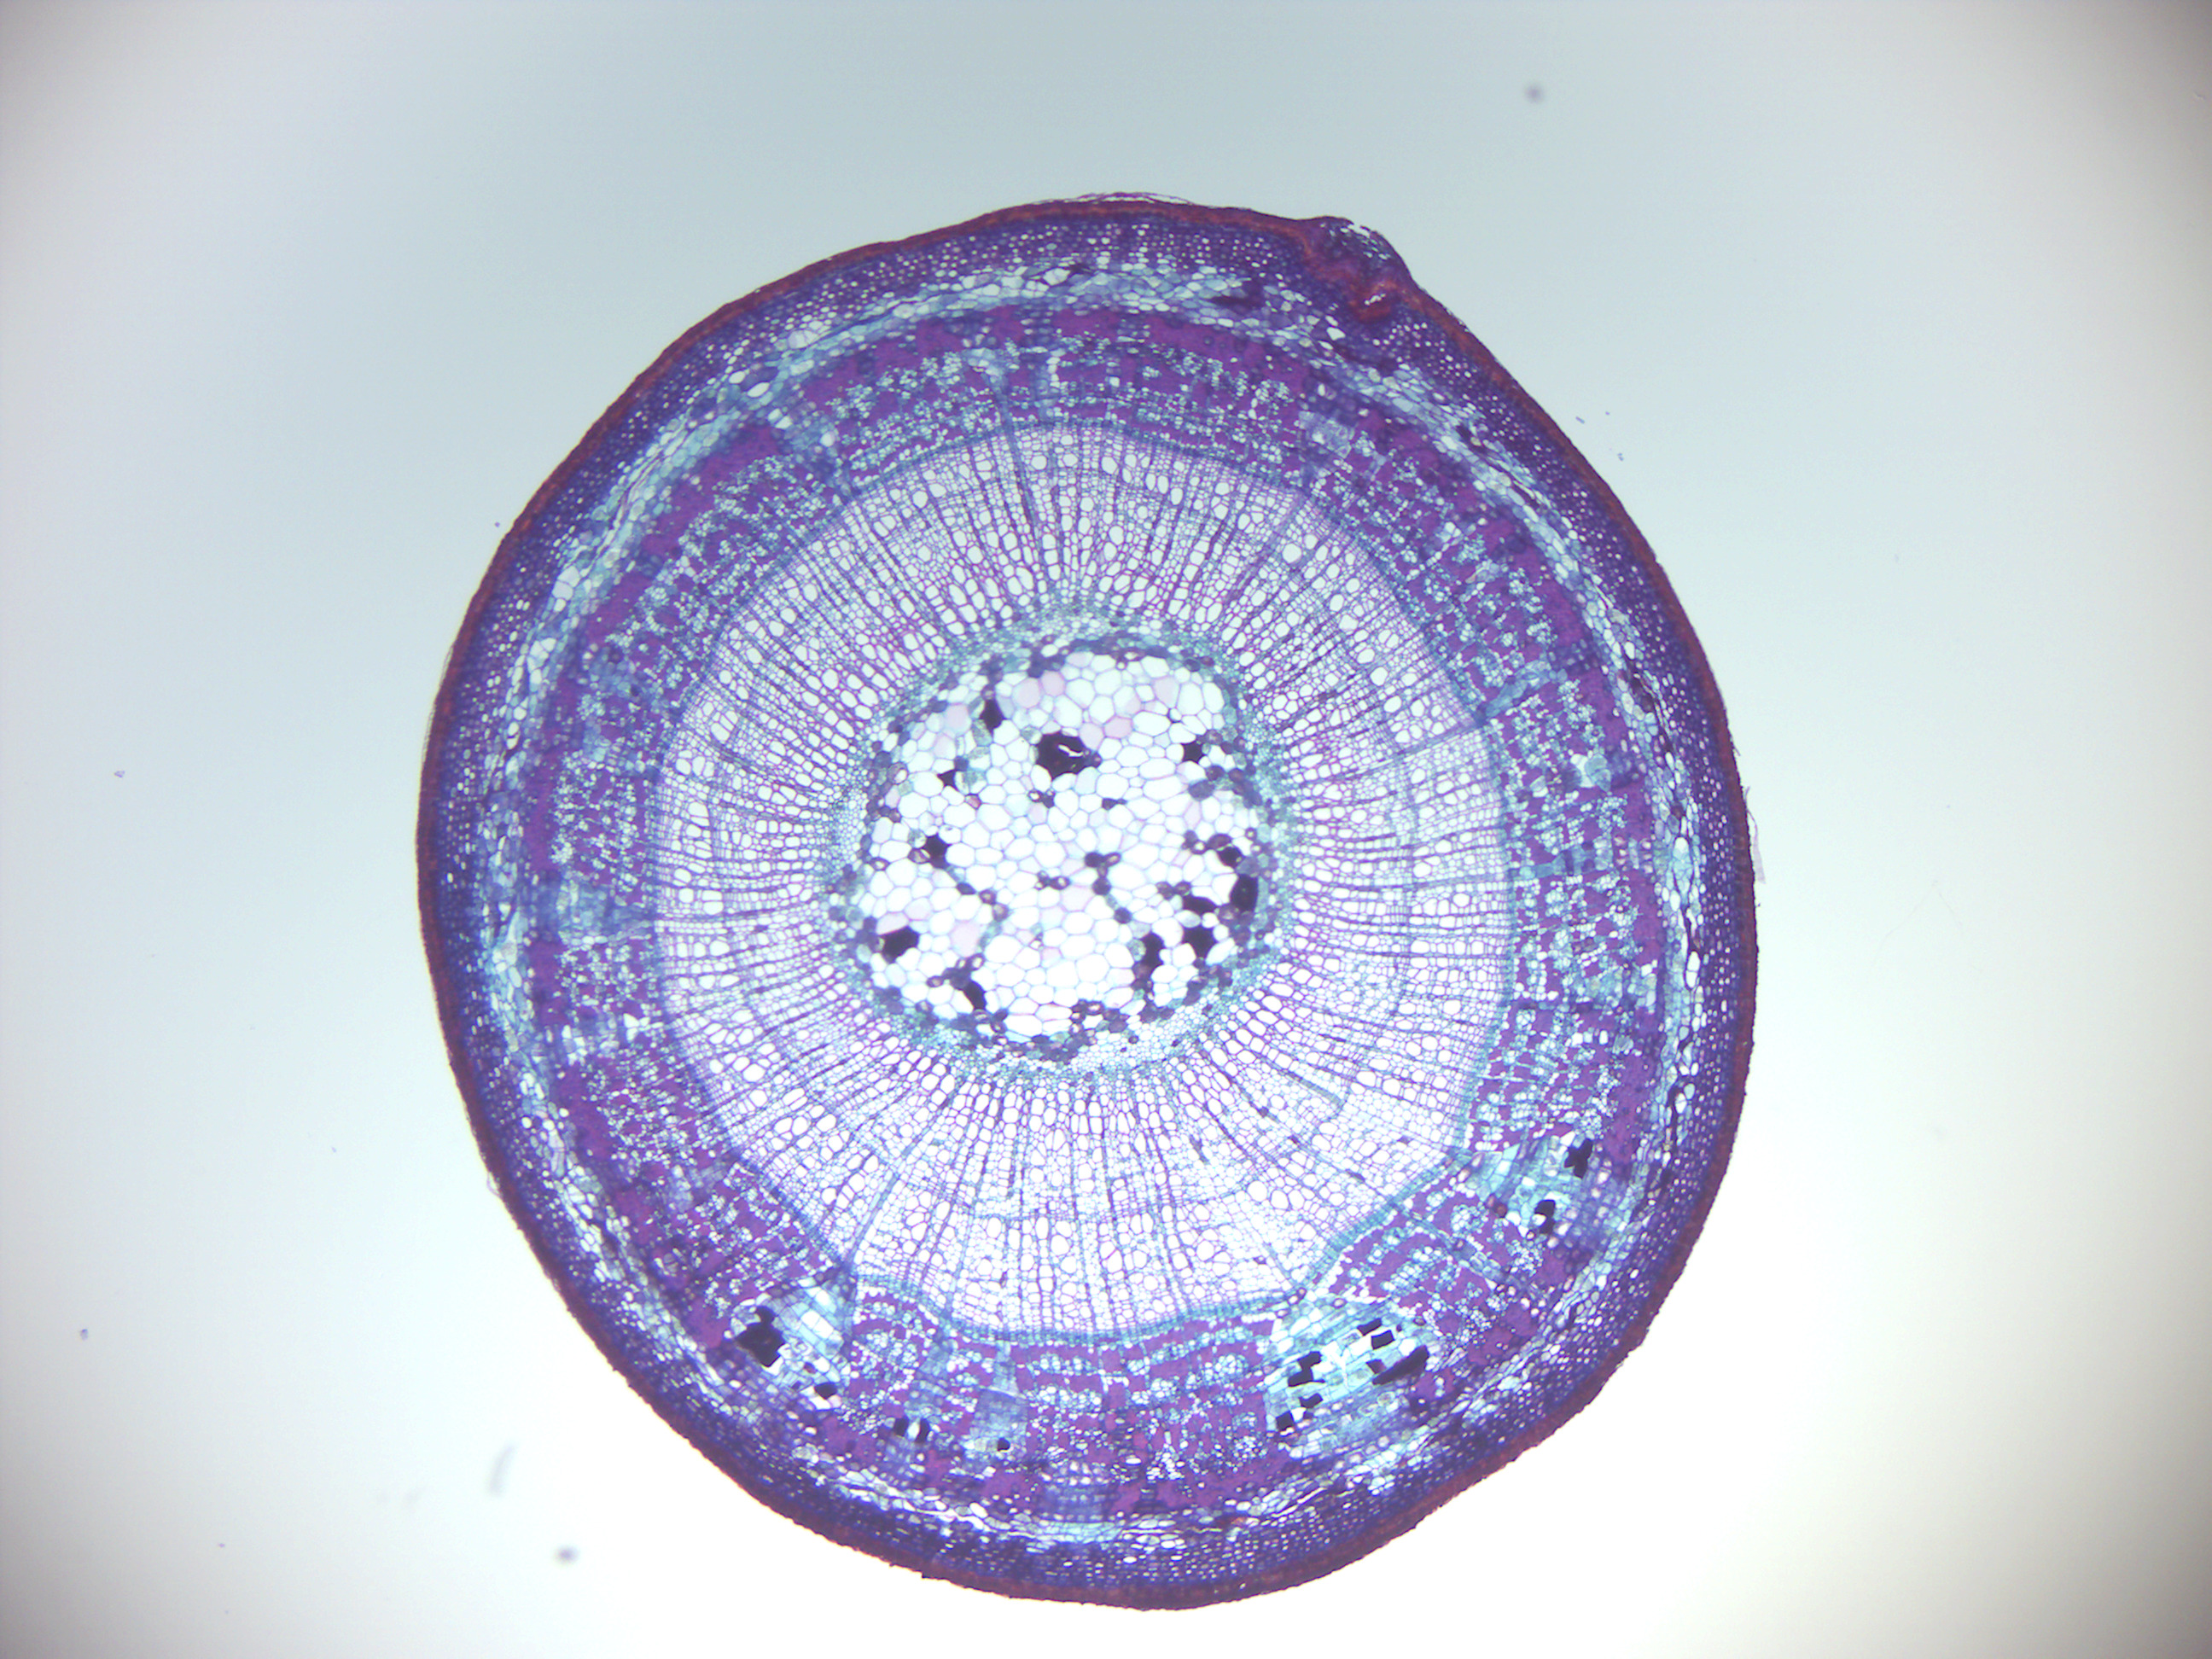
\includegraphics[width=0.7\linewidth]{./figures/gymnosperms/tilia}

}

\caption{\emph{Tilia} 2 year old stem}\label{fig:tilia}
\end{figure}

\begin{figure}

{\centering 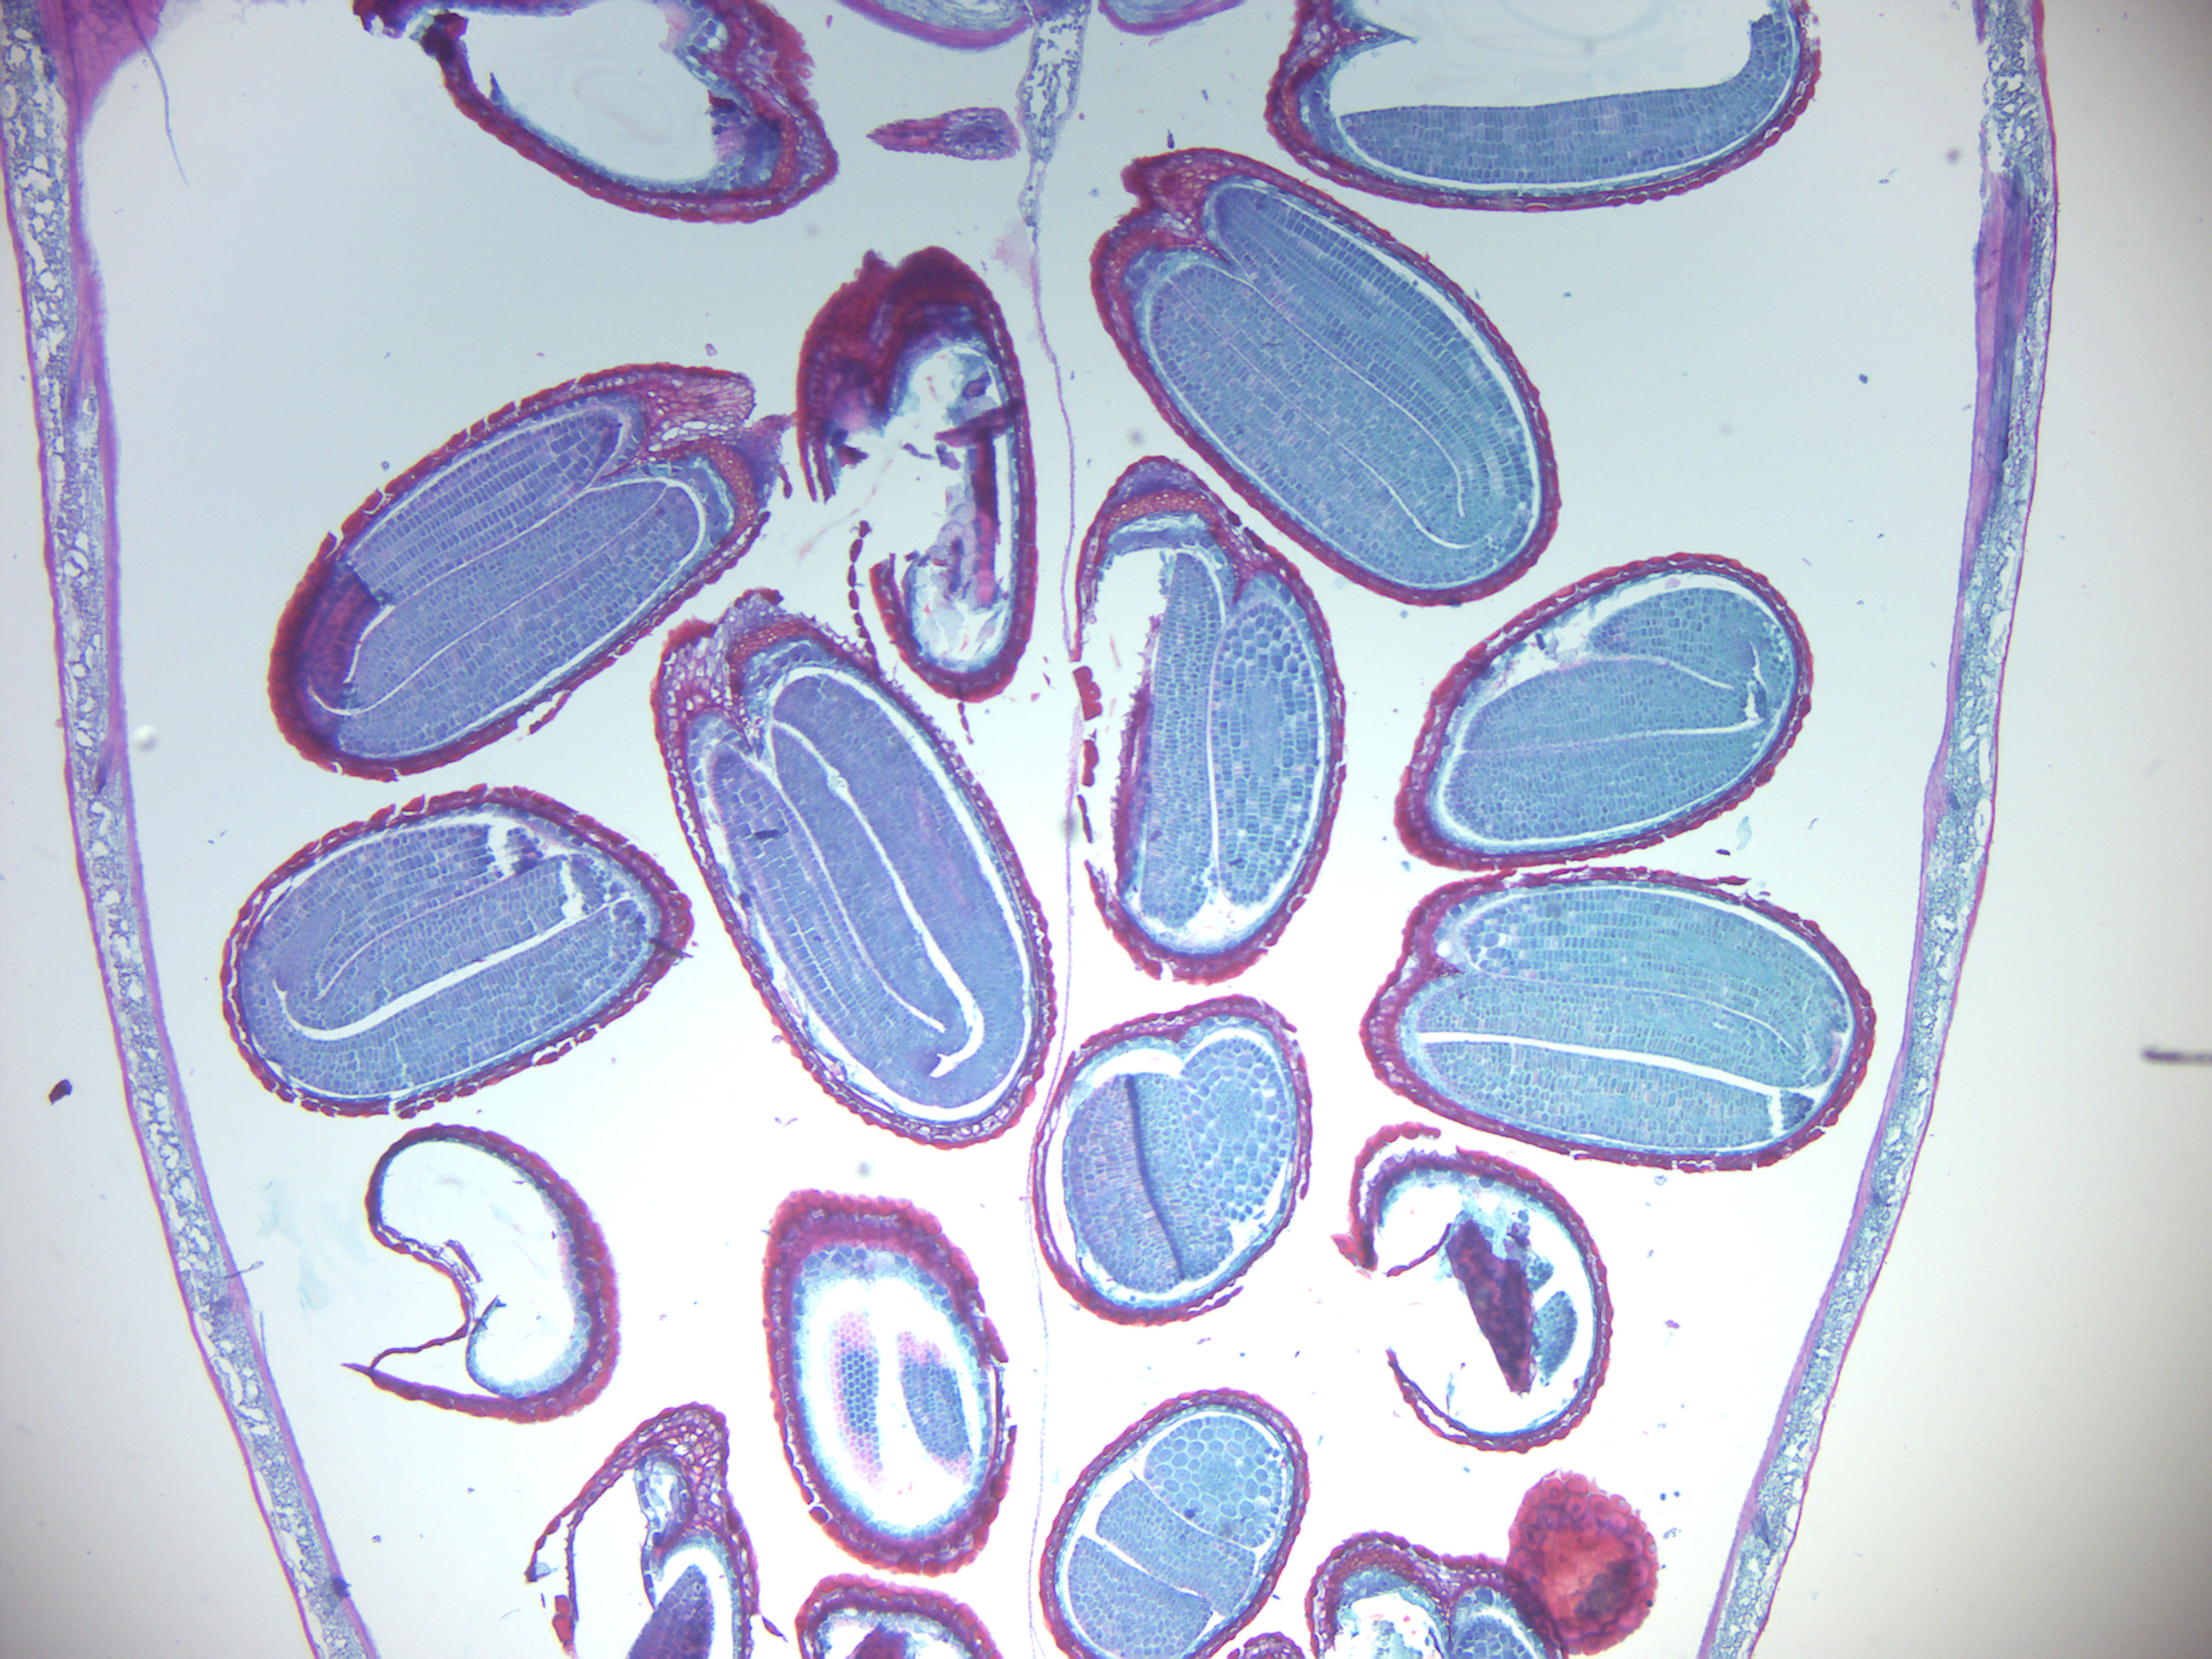
\includegraphics[width=0.7\linewidth]{./figures/gymnosperms/capsella_embryo}

}

\caption{\emph{Capsella} seeds.}\label{fig:capsella}
\end{figure}

\section{Monocotyledons and
Dicotyledons}\label{monocotyledons-and-dicotyledons}

Monocotyledons, commonly referred to as monocots are flowering plants
(angiosperms) whose seeds typically contain only one embryonic leaf, or
cotyledon. They constitute one of the major groups into which the
flowering plants have traditionally been divided, the rest of the
flowering plants having two cotyledons and therefore classified as
dicotyledons, or dicots. However, molecular phylogenetic research has
shown that while the monocots form a monophyletic group or clade
(comprising all the descendants of a common ancestor), the dicots do
not.

The eudicots, eudicotyledons are a monophyletic clade of flowering
plants. The term means ``true dicotyledons'', as it contains the
majority of plants that have been considered dicots and have
characteristics of the dicots. The term ``eudicots'' has subsequently
been widely adopted in botany to refer to one of the two largest clades
of angiosperms (constituting over 70\% of the angiosperm species),
monocots being the other.

\begin{table}[h!]
\centering
\caption{Structural differences between monocots and
dicots.}\label{tab:moncots}
\begin{tabularx}{\columnwidth}{YYY} \\
\toprule
Feature & In monocots & In dicots \\
\midrule
Leaves &
Leaf shape oblong or linear, often sheathed at base, petiole seldom
developed, stipules absent. Major leaf veins usually parallel. &
Broad, seldom sheathed, petiole common often with stipules. Veins
usually reticulate (pinnate or palmate).\\
Roots &
Primary root of short duration, replaced by adventitial roots forming
fibrous or fleshy root systems. &
Develops from the radicle. Primary root often persists forming strong
taproot and secondary roots. \\
Plant stem: Vascular bundles &
Numerous scattered bundles in ground parenchyma, cambium rarely present,
no differentiation between cortical and stelar regions. & Ring of primary bundles with cambium, differentiated into cortex and
stele (eustelic).\\
Flowers & Parts in threes or multiples of three (e.g.~3, 6 or 9 petals) & Parts in fours or fives.\\
\bottomrule \\
\end{tabularx}
\end{table}

\section{View Prepared Slides of Monocots And
Eudicots}\label{view-prepared-slides-of-monocots-and-eudicots}

\begin{enumerate}
\def\labelenumi{\arabic{enumi}.}
\tightlist
\item
  Monocot and dicot roots (Figures \ref{fig:monocotroot} and
  \ref{fig:dicotroot})

  \begin{itemize}
  \tightlist
  \item
    Identify monocot and eudicot root.
  \end{itemize}
\item
  Monocot and dicot stems (Figures \ref{fig:monocotstem} and
  \ref{fig:dicotstem})

  \begin{itemize}
  \tightlist
  \item
    Identify monocot and eudicot sterm.
  \end{itemize}
\item
  Monocot and dicot leaves (Figures \ref{fig:monocotleave} and
  \ref{fig:dicotleave})

  \begin{itemize}
  \tightlist
  \item
    Identify monocot and eudicot leaf.
  \end{itemize}
\item
  Monocot and dicot flower buds (Figures \ref{fig:monocotbud} and
  \ref{fig:dicotbud})

  \begin{itemize}
  \tightlist
  \item
    Identify monocot and eudicot flower.
  \end{itemize}
\end{enumerate}

\begin{figure}

{\centering 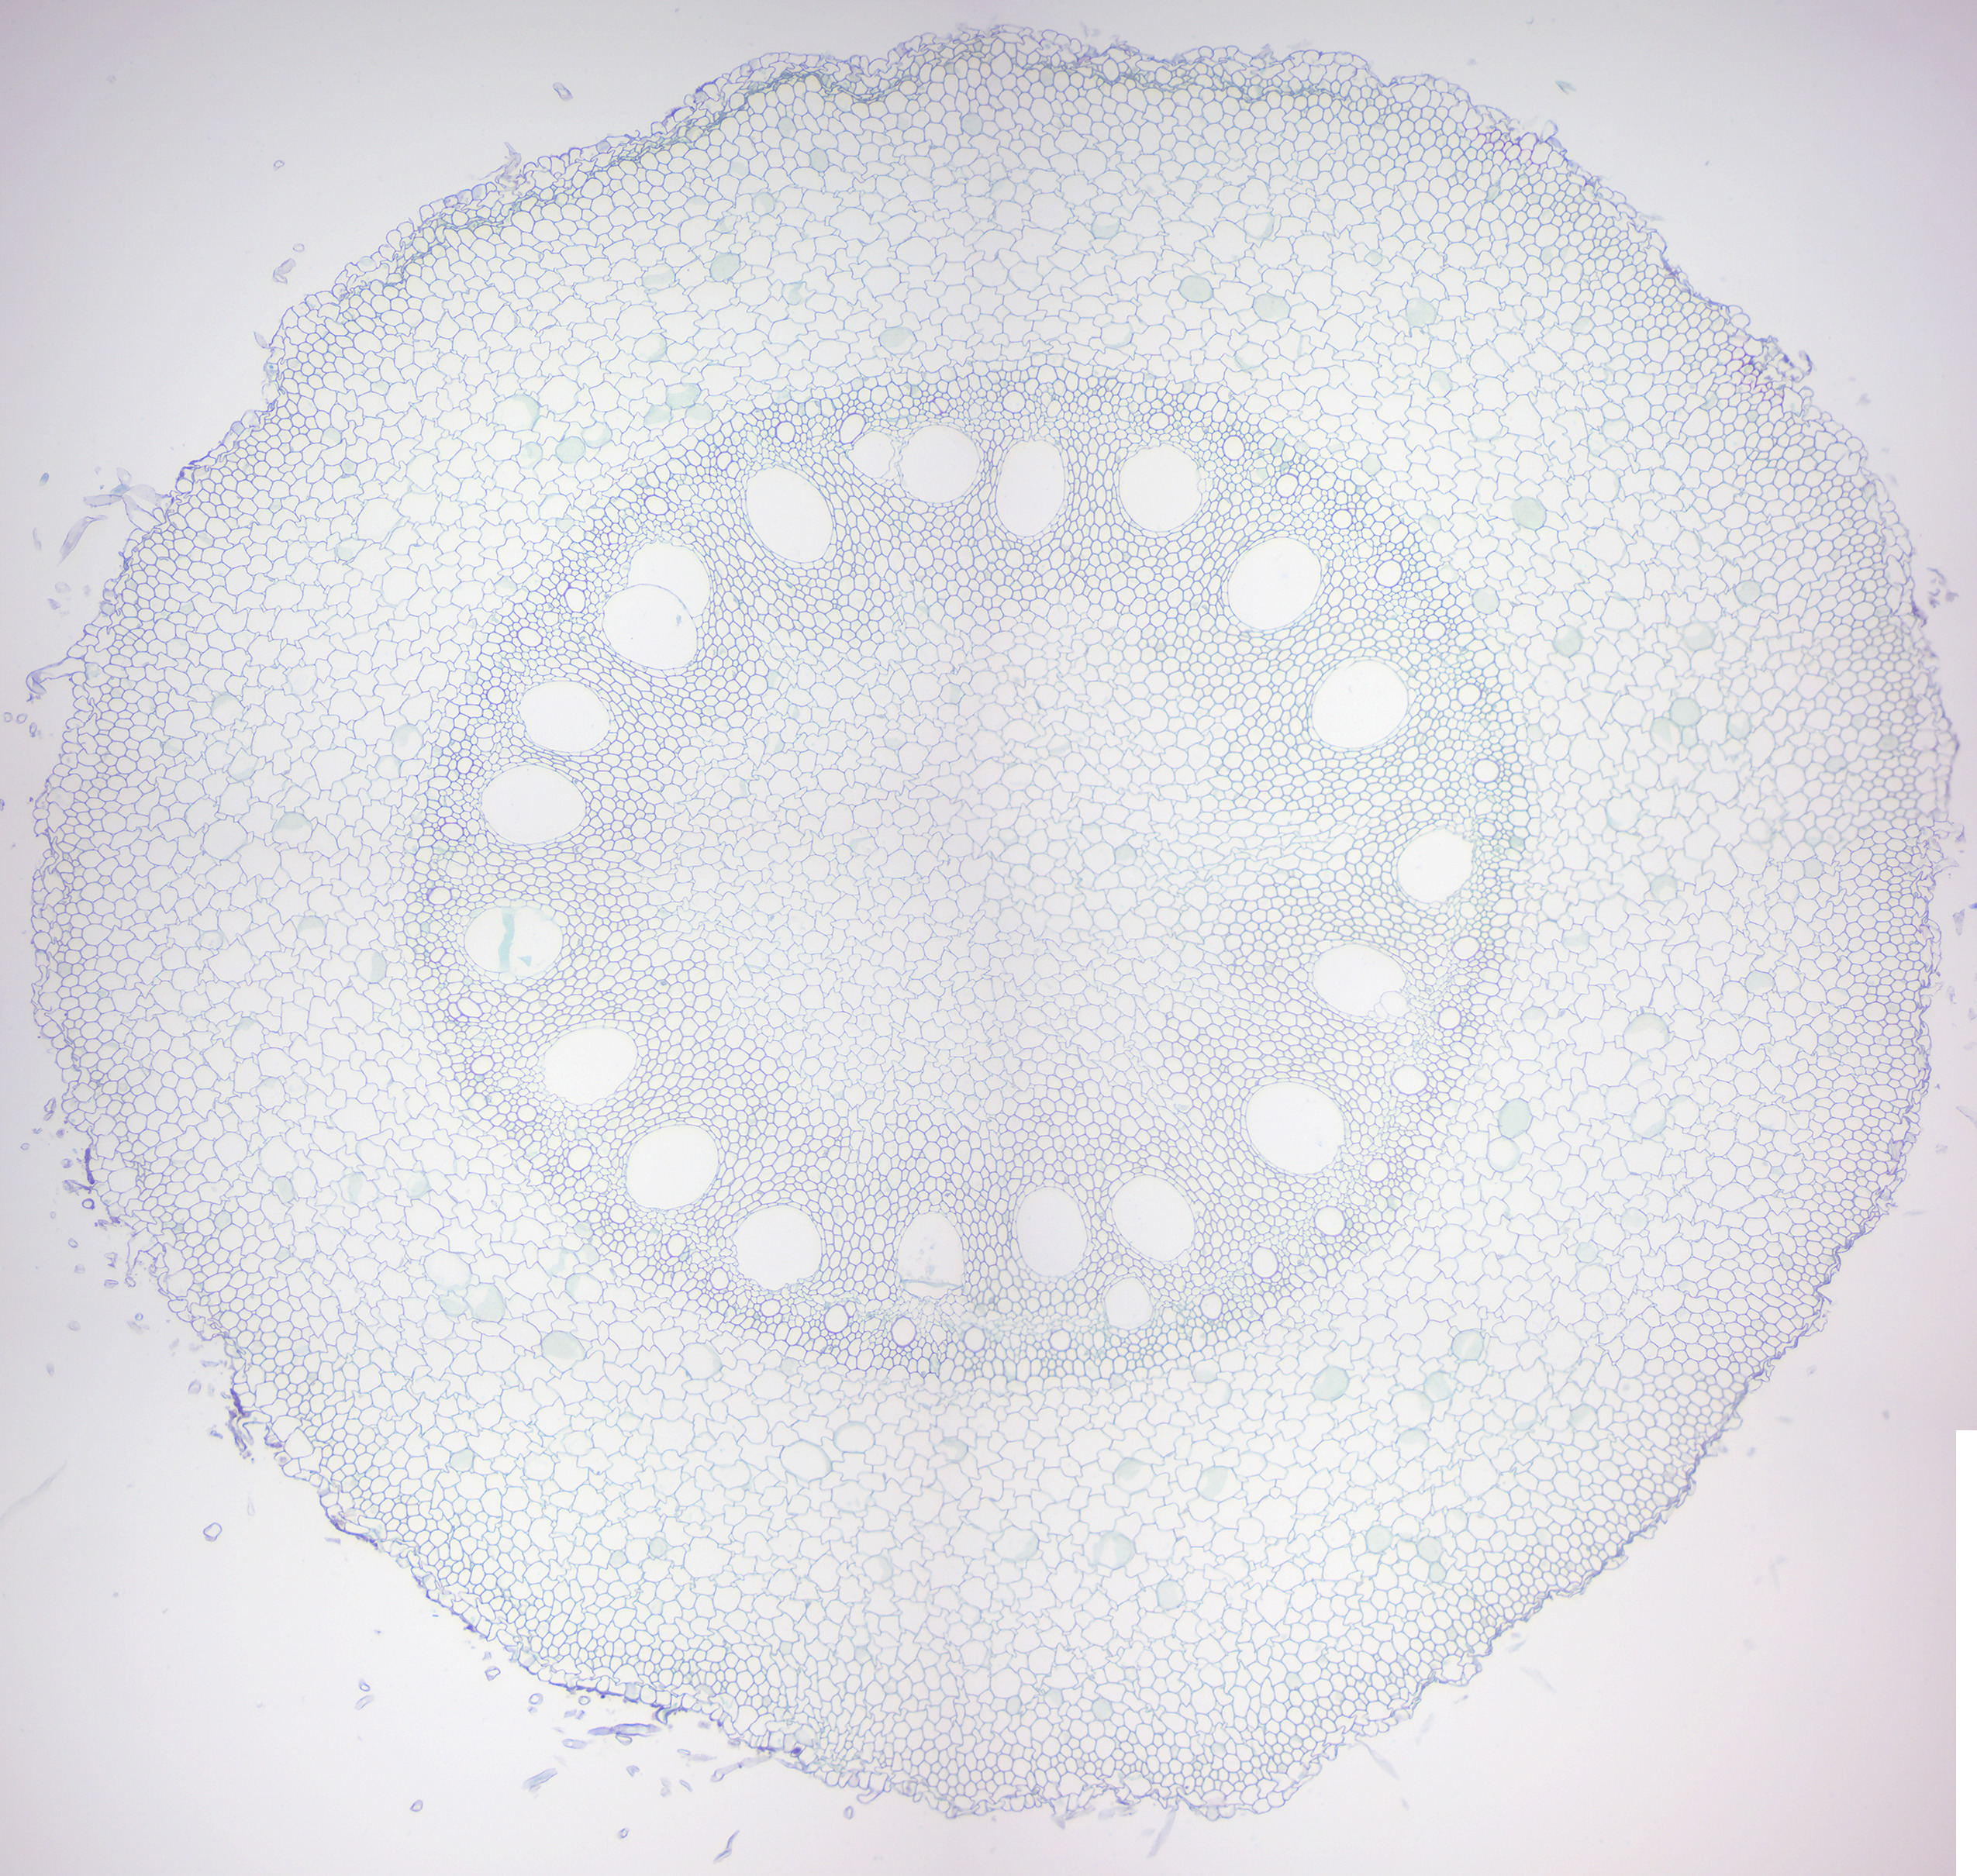
\includegraphics[width=0.7\linewidth]{./figures/gymnosperms/monocot_root}

}

\caption{Monocot root.}\label{fig:monocotroot}
\end{figure}

\begin{figure}

{\centering 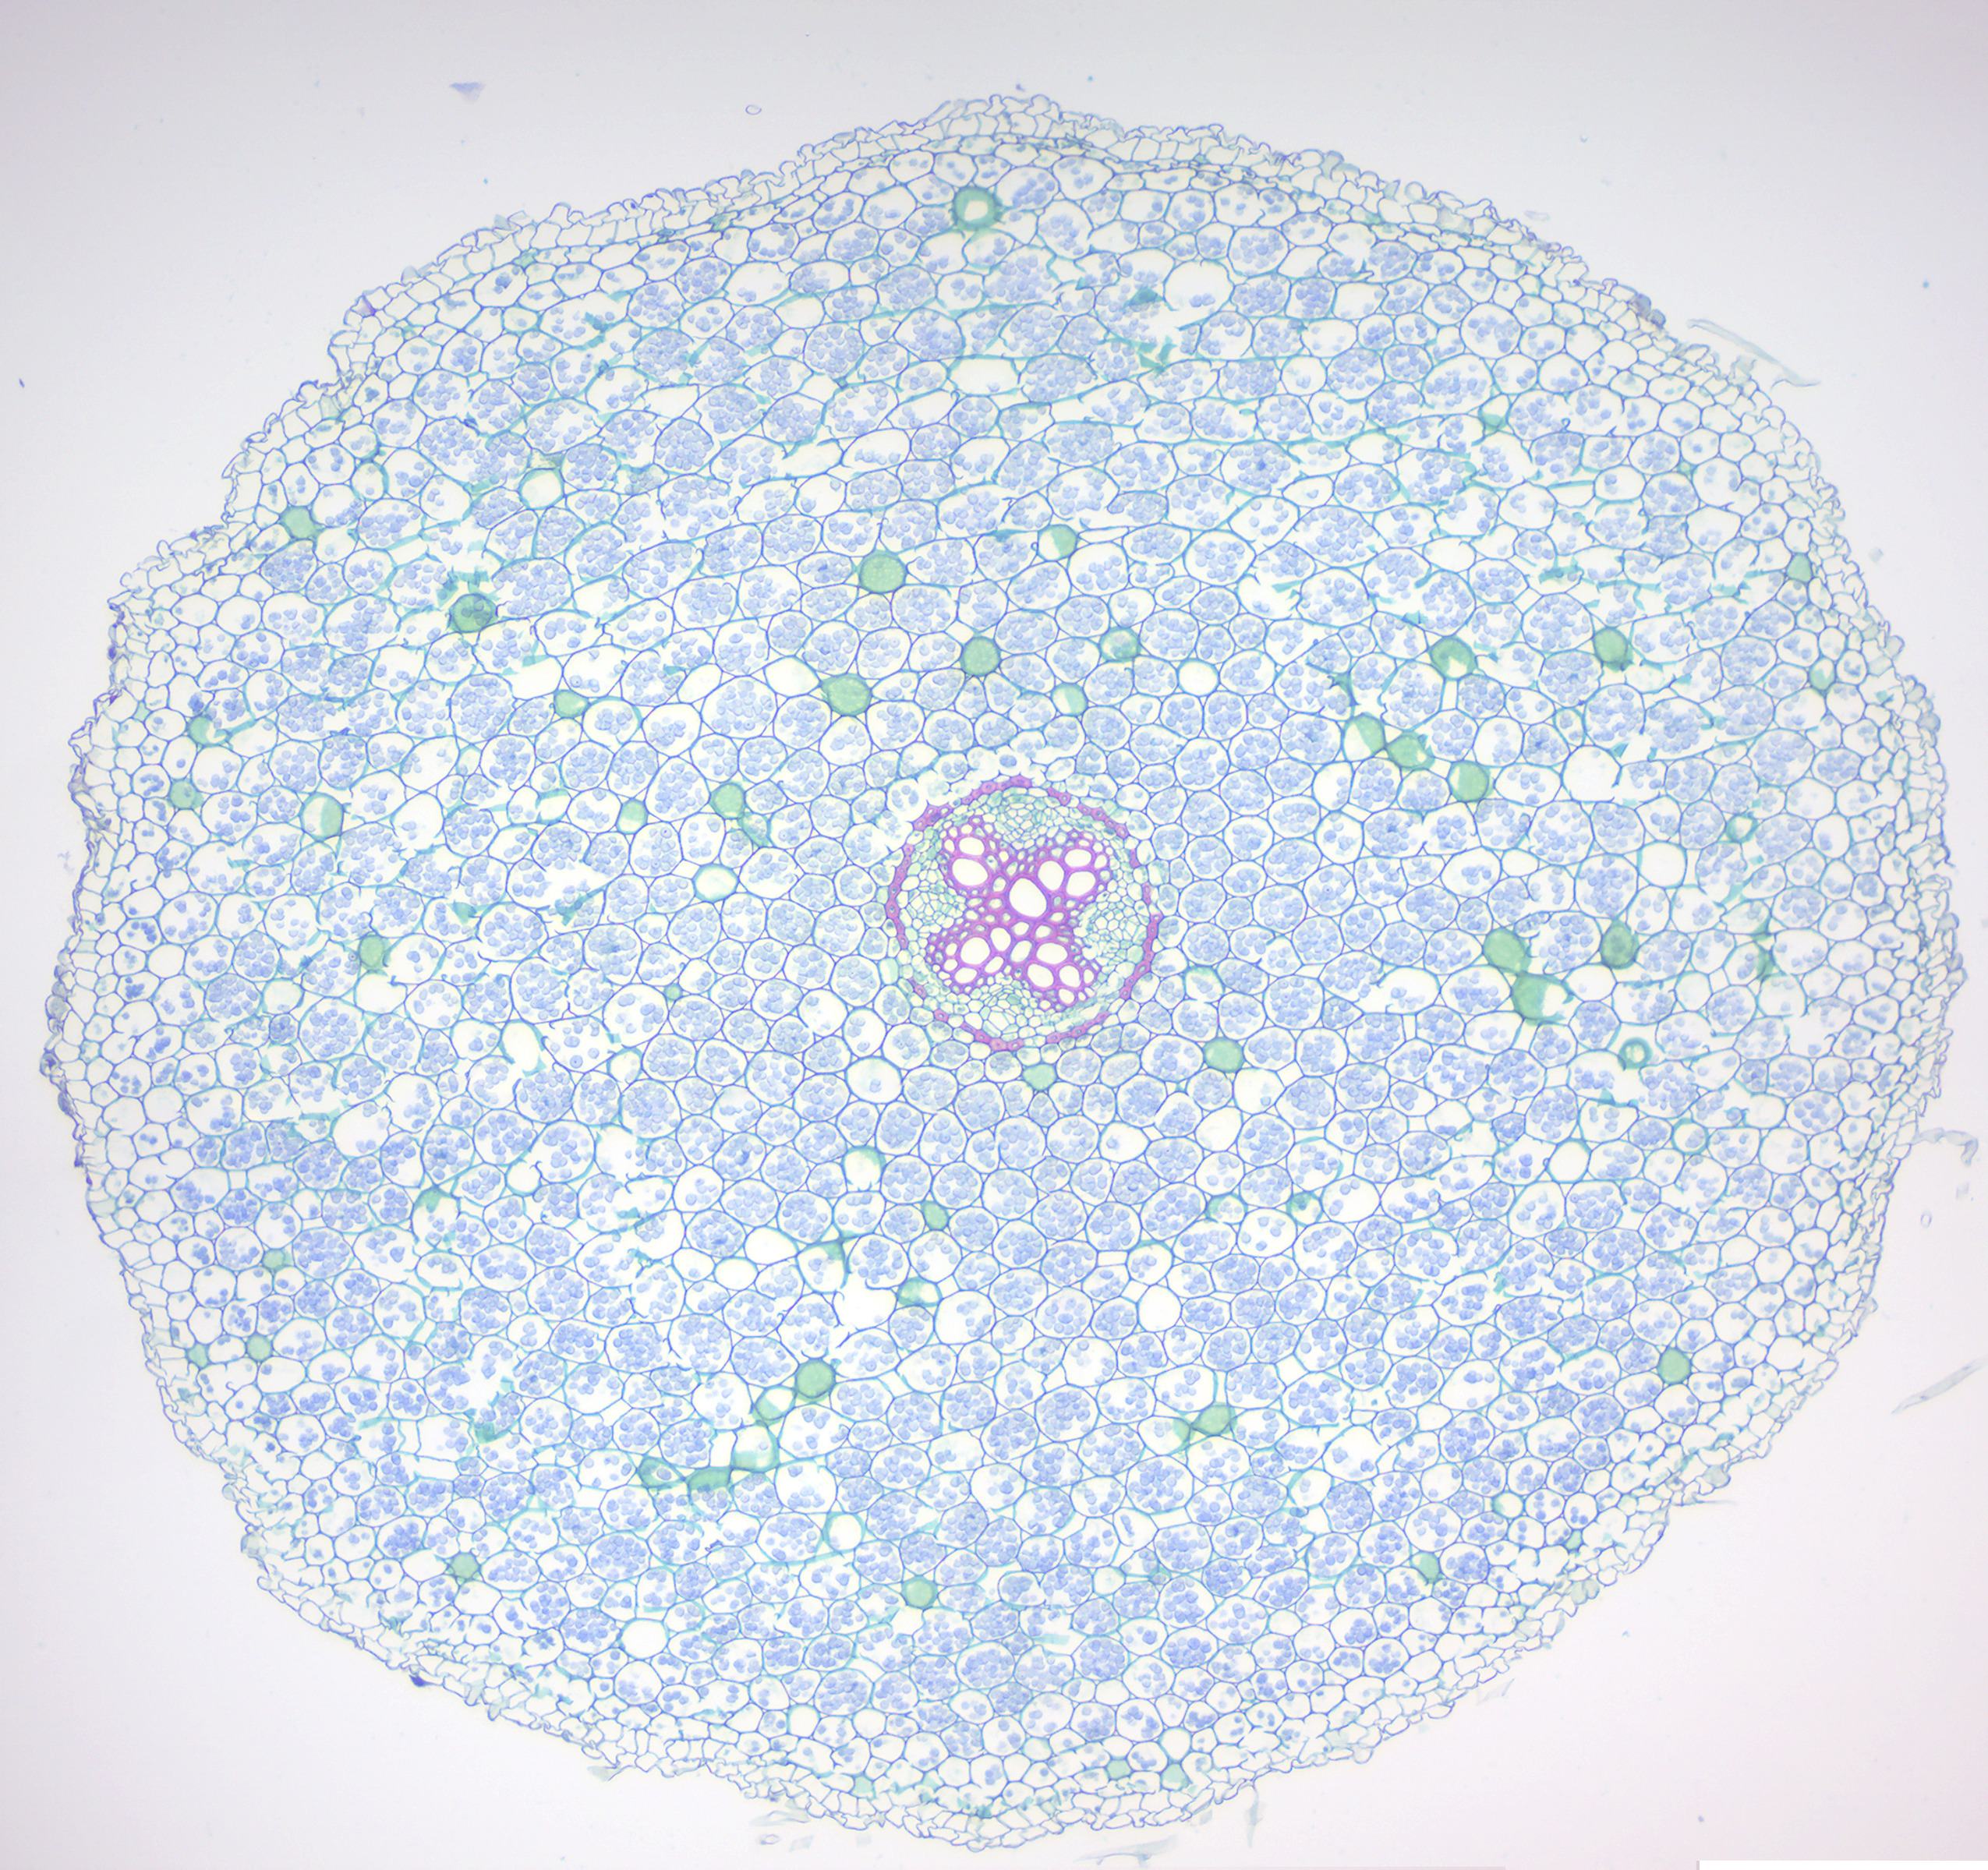
\includegraphics[width=0.7\linewidth]{./figures/gymnosperms/Dicot_root}

}

\caption{Dicot root.}\label{fig:dicotroot}
\end{figure}

\begin{figure}

{\centering 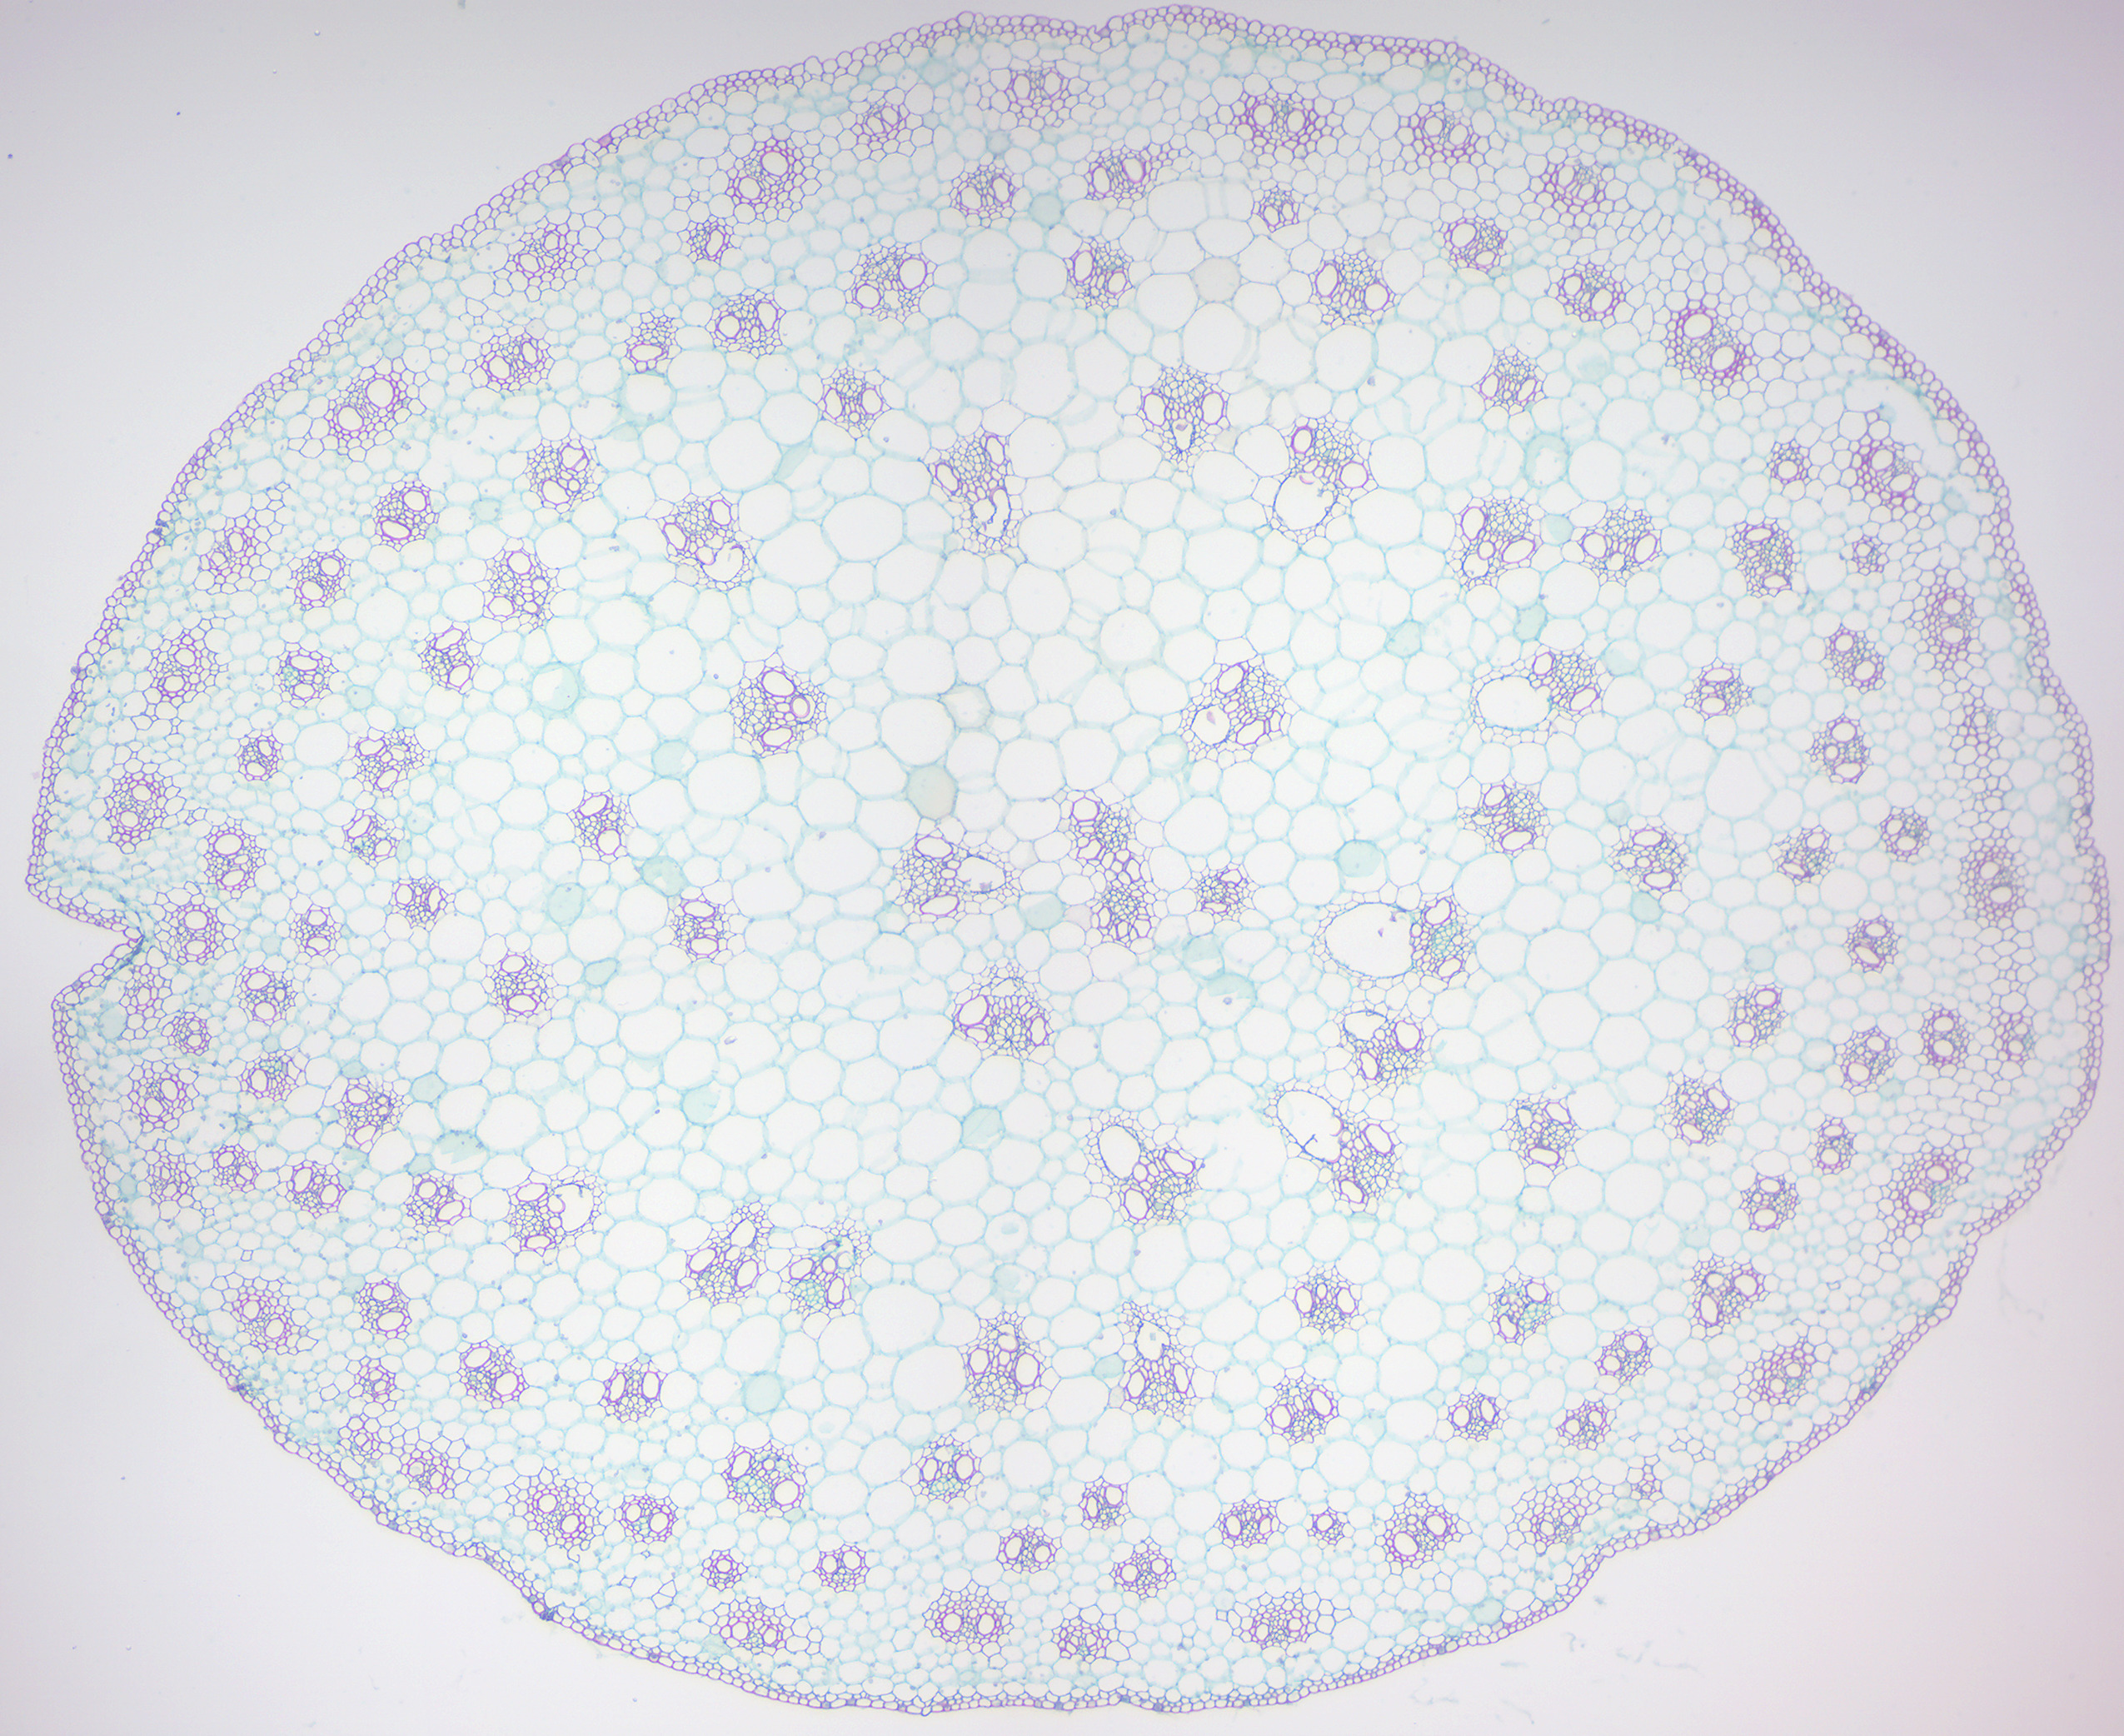
\includegraphics[width=0.7\linewidth]{./figures/gymnosperms/monocot_stem}

}

\caption{Monocot stem.}\label{fig:monocotstem}
\end{figure}

\begin{figure}

{\centering 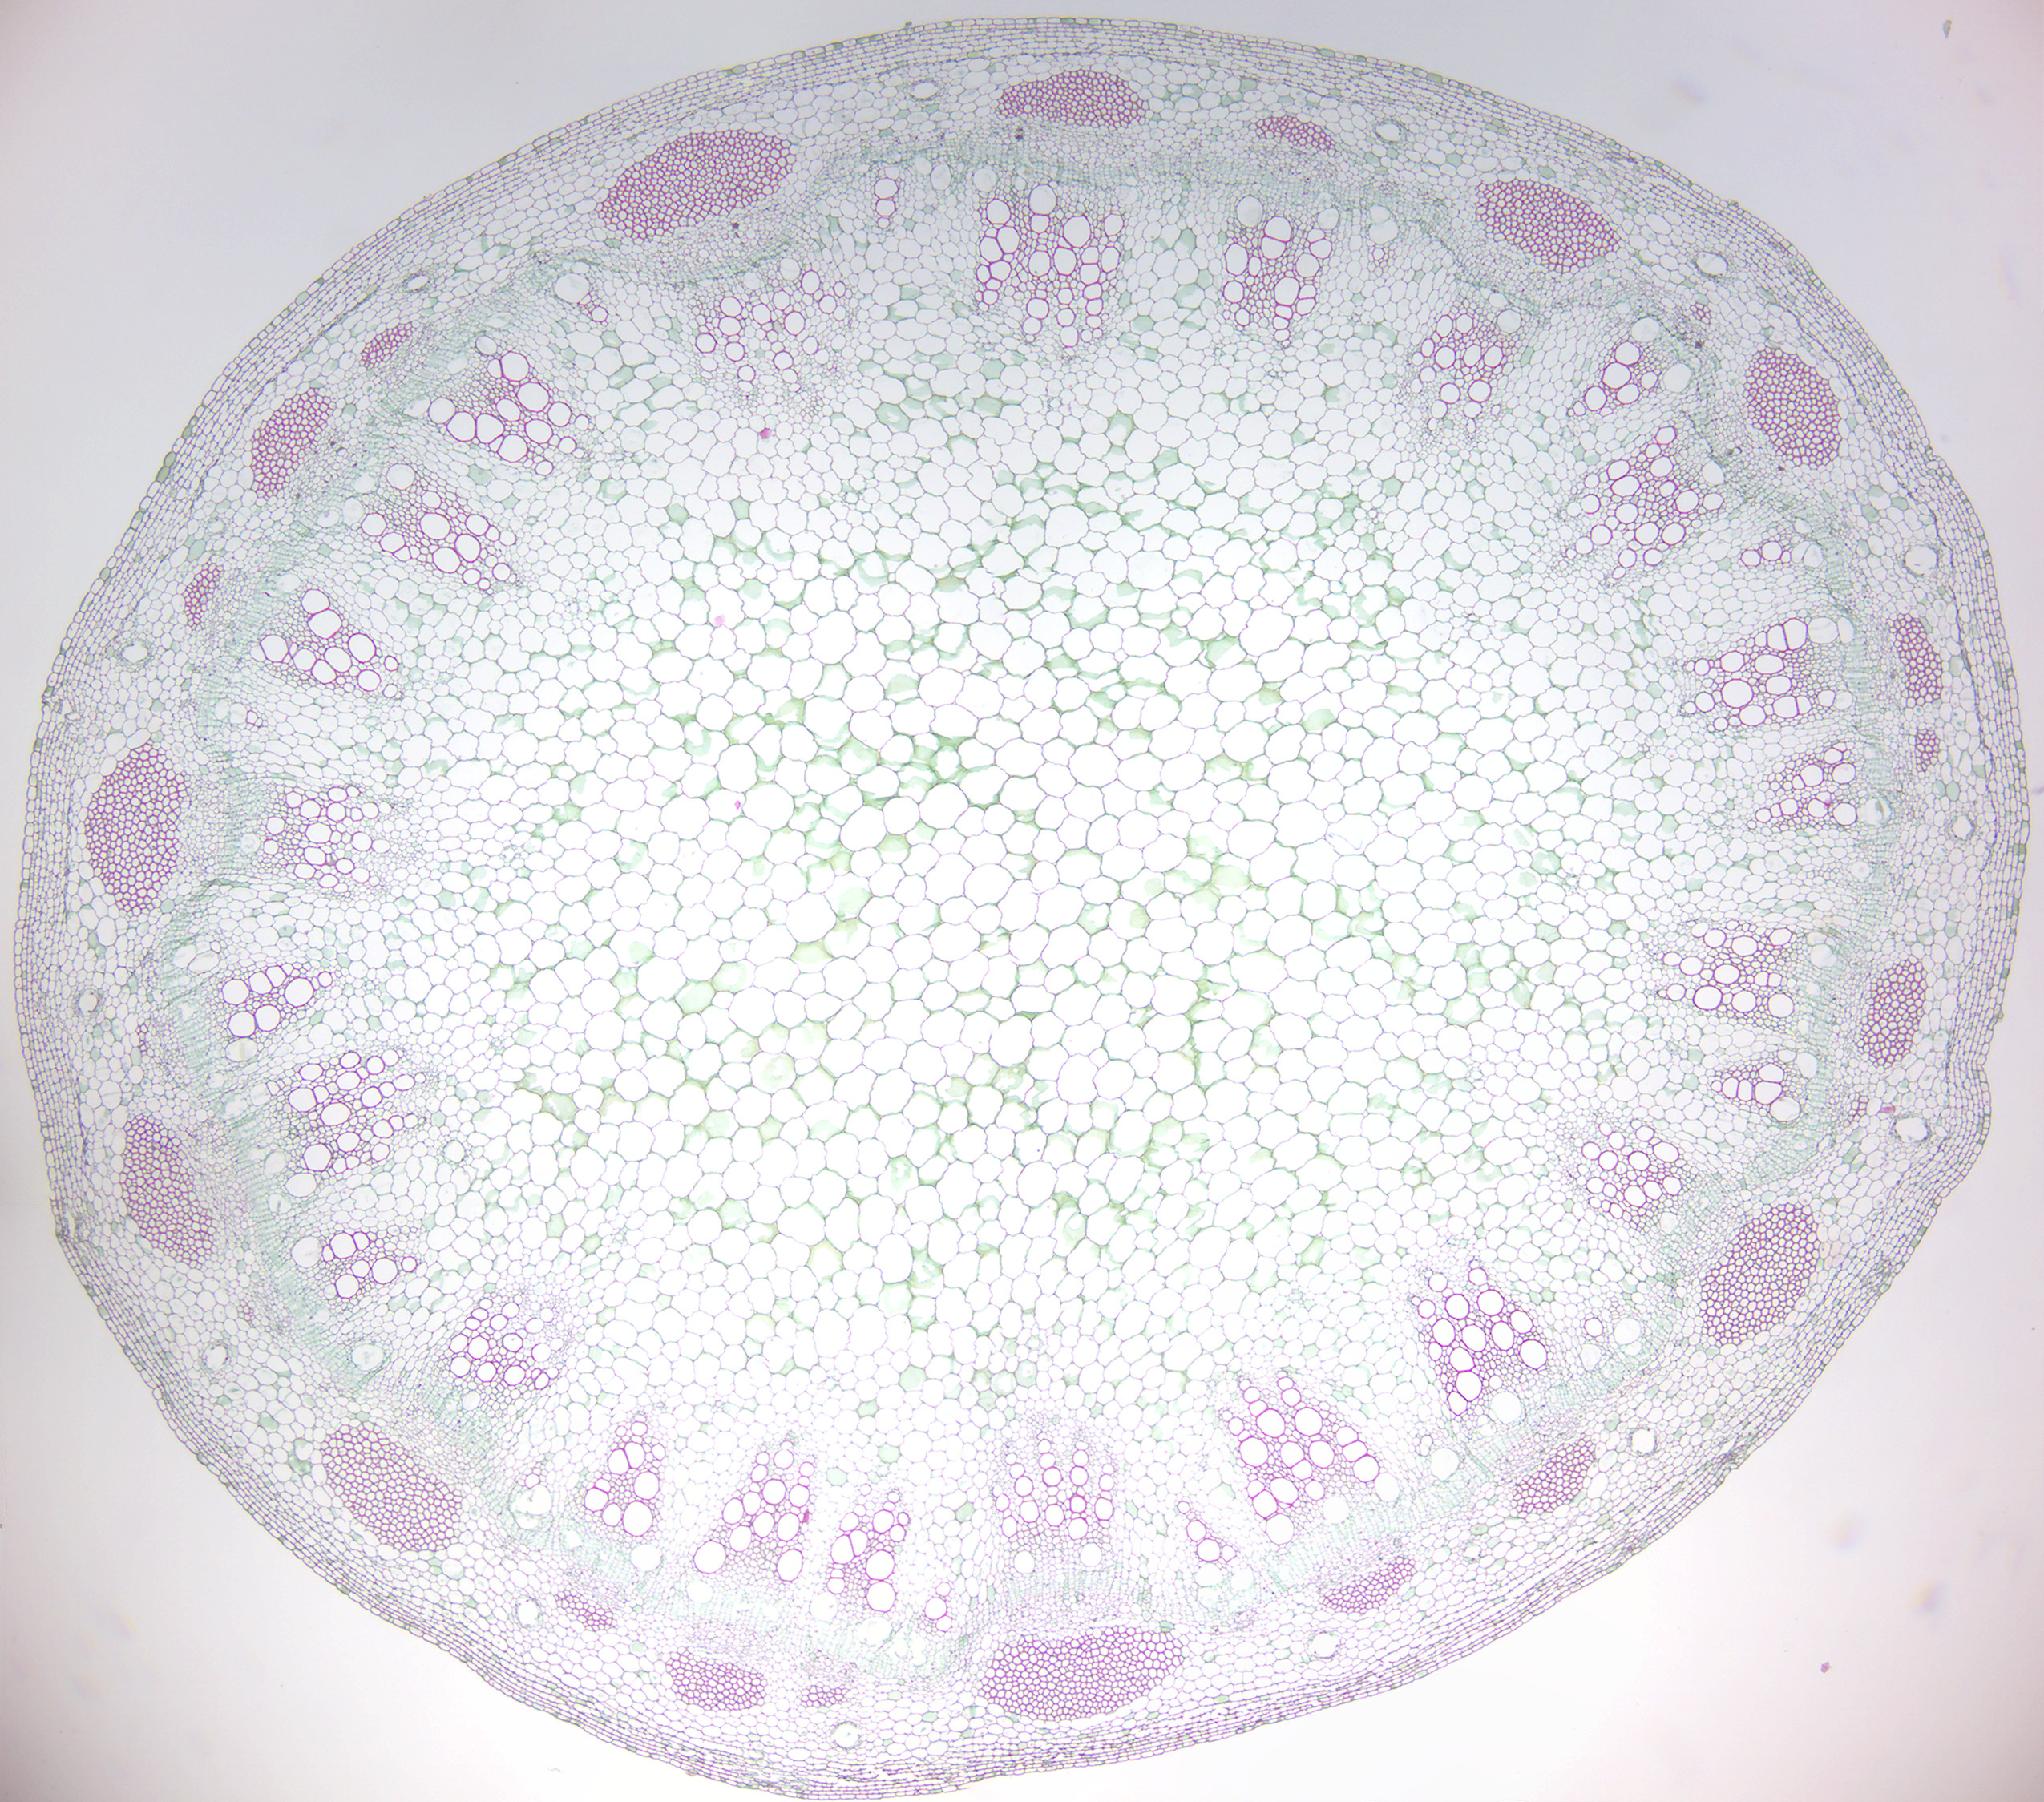
\includegraphics[width=0.7\linewidth]{./figures/gymnosperms/dicot_stem}

}

\caption{Dicot stem}\label{fig:dicotstem}
\end{figure}

\begin{figure}

{\centering 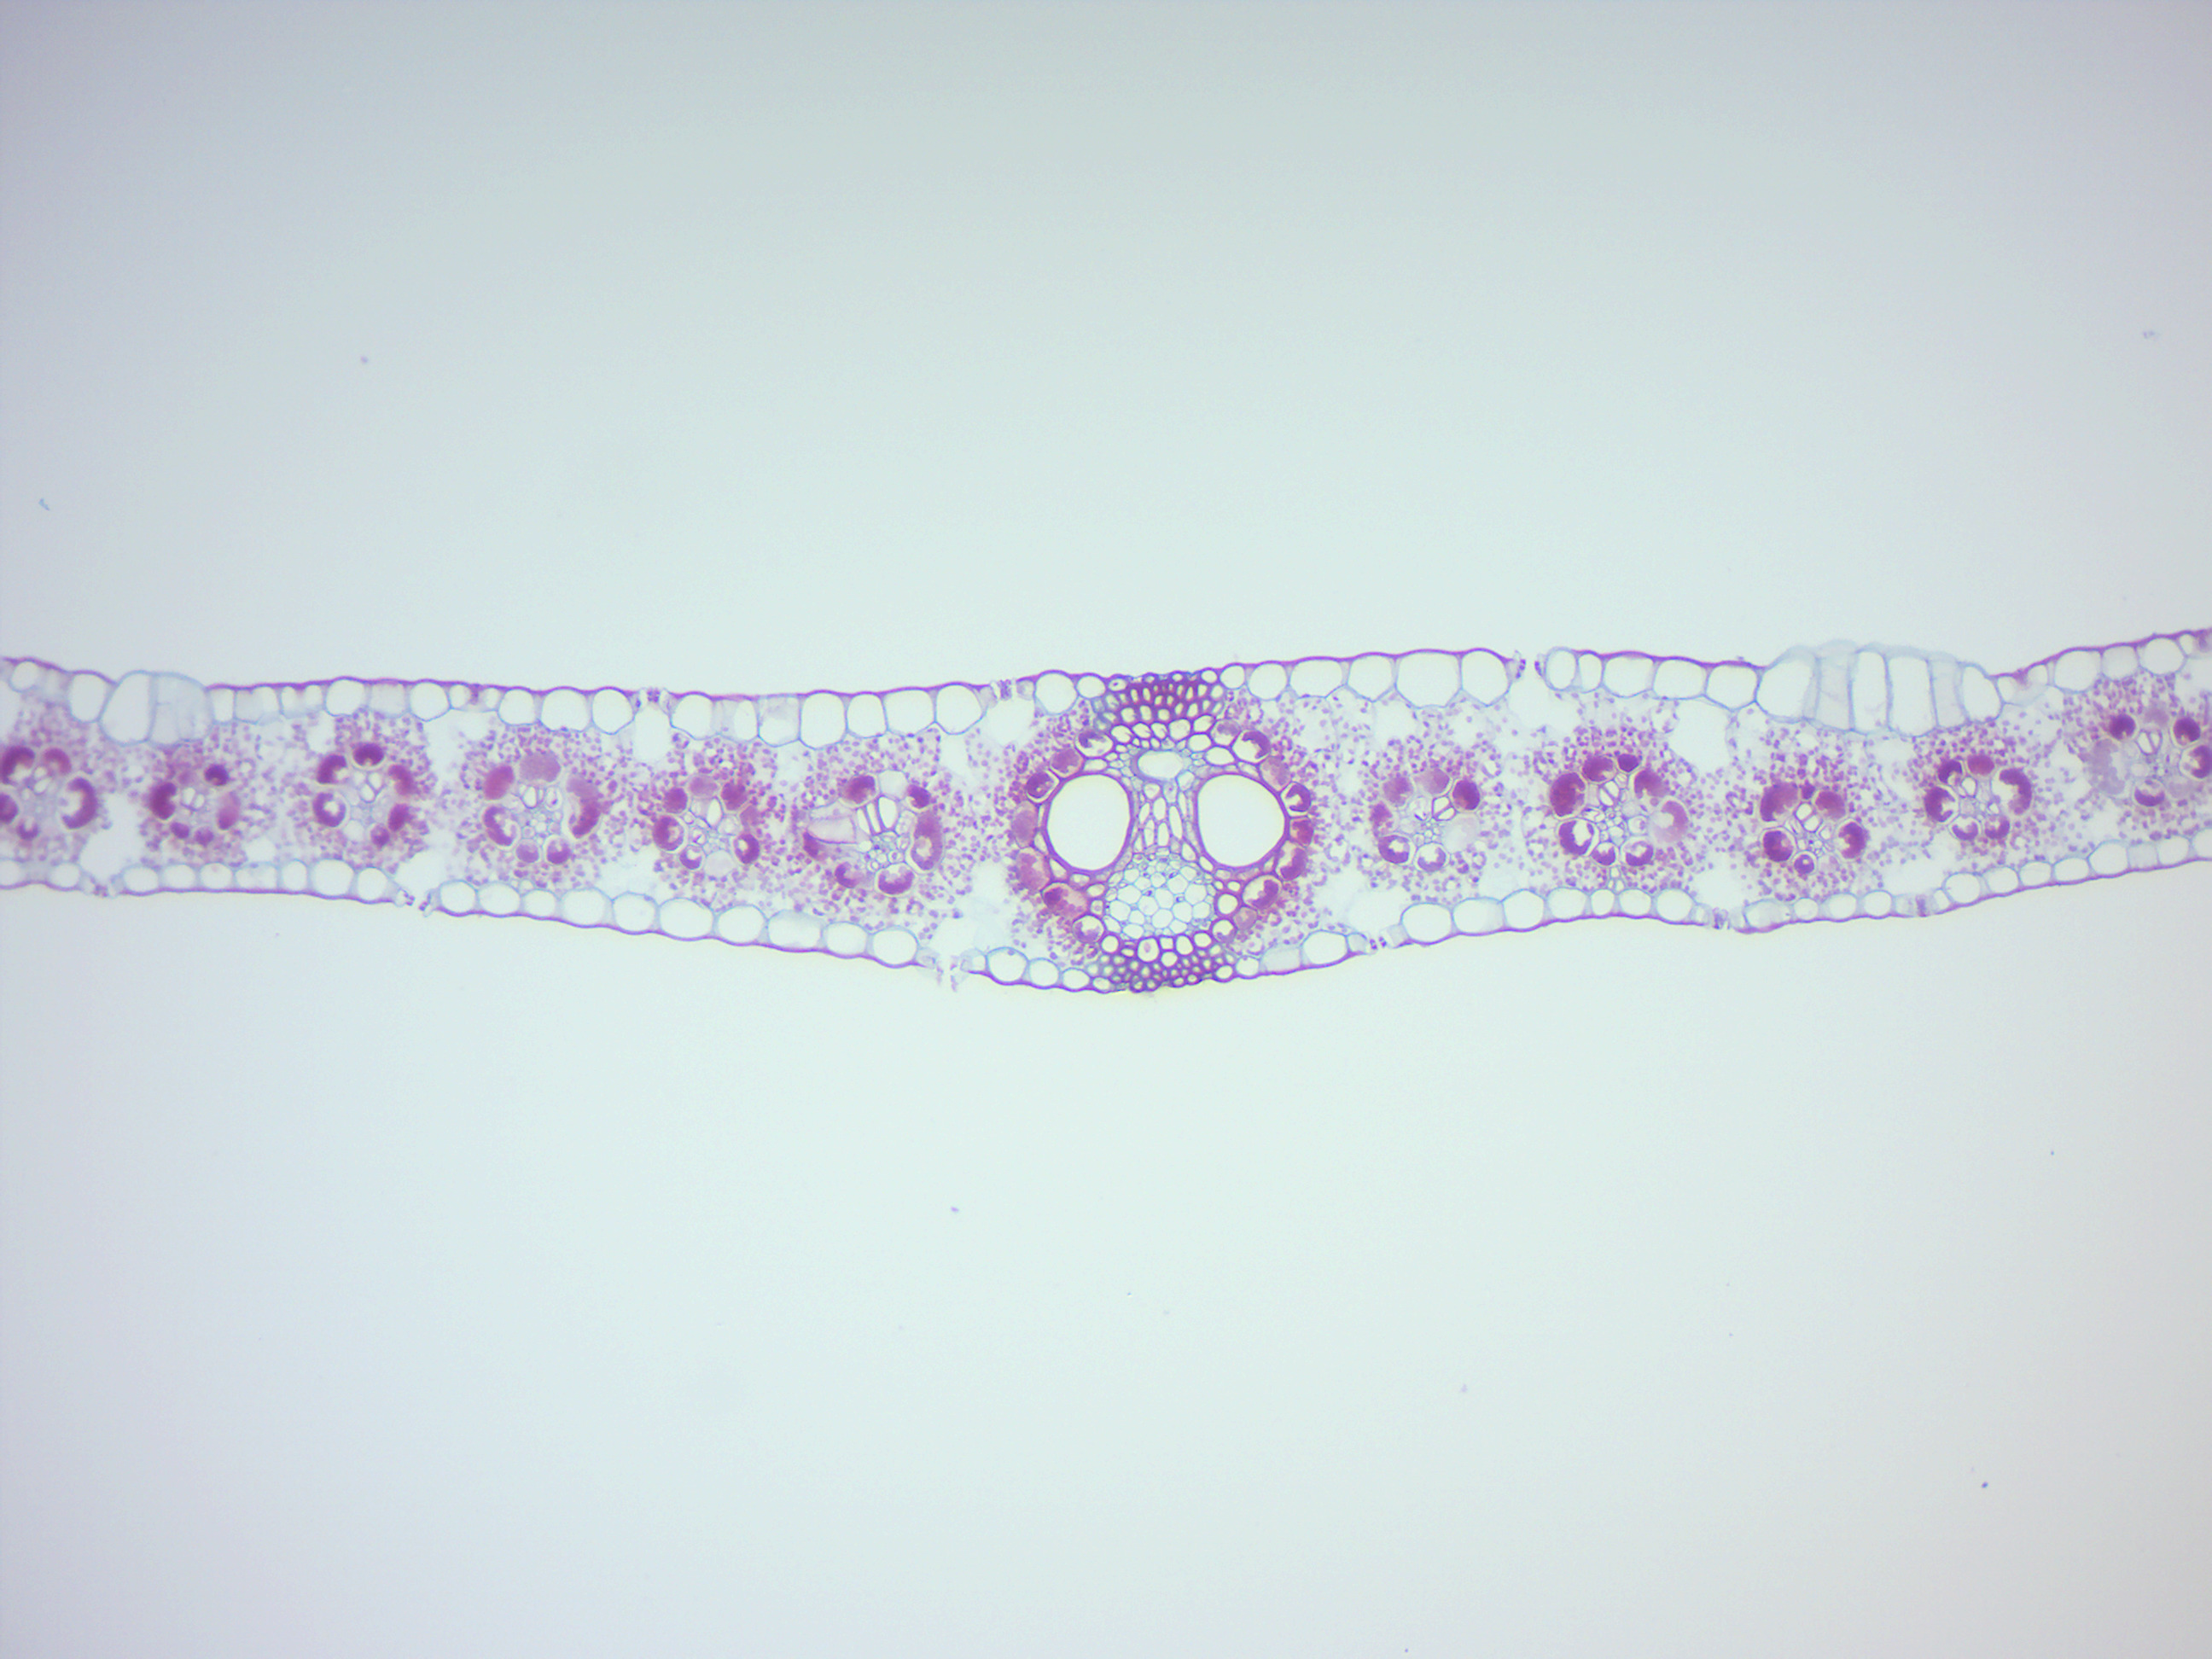
\includegraphics[width=0.7\linewidth]{./figures/gymnosperms/monocot_leave}

}

\caption{Monocot leave.}\label{fig:monocotleave}
\end{figure}

\begin{figure}

{\centering 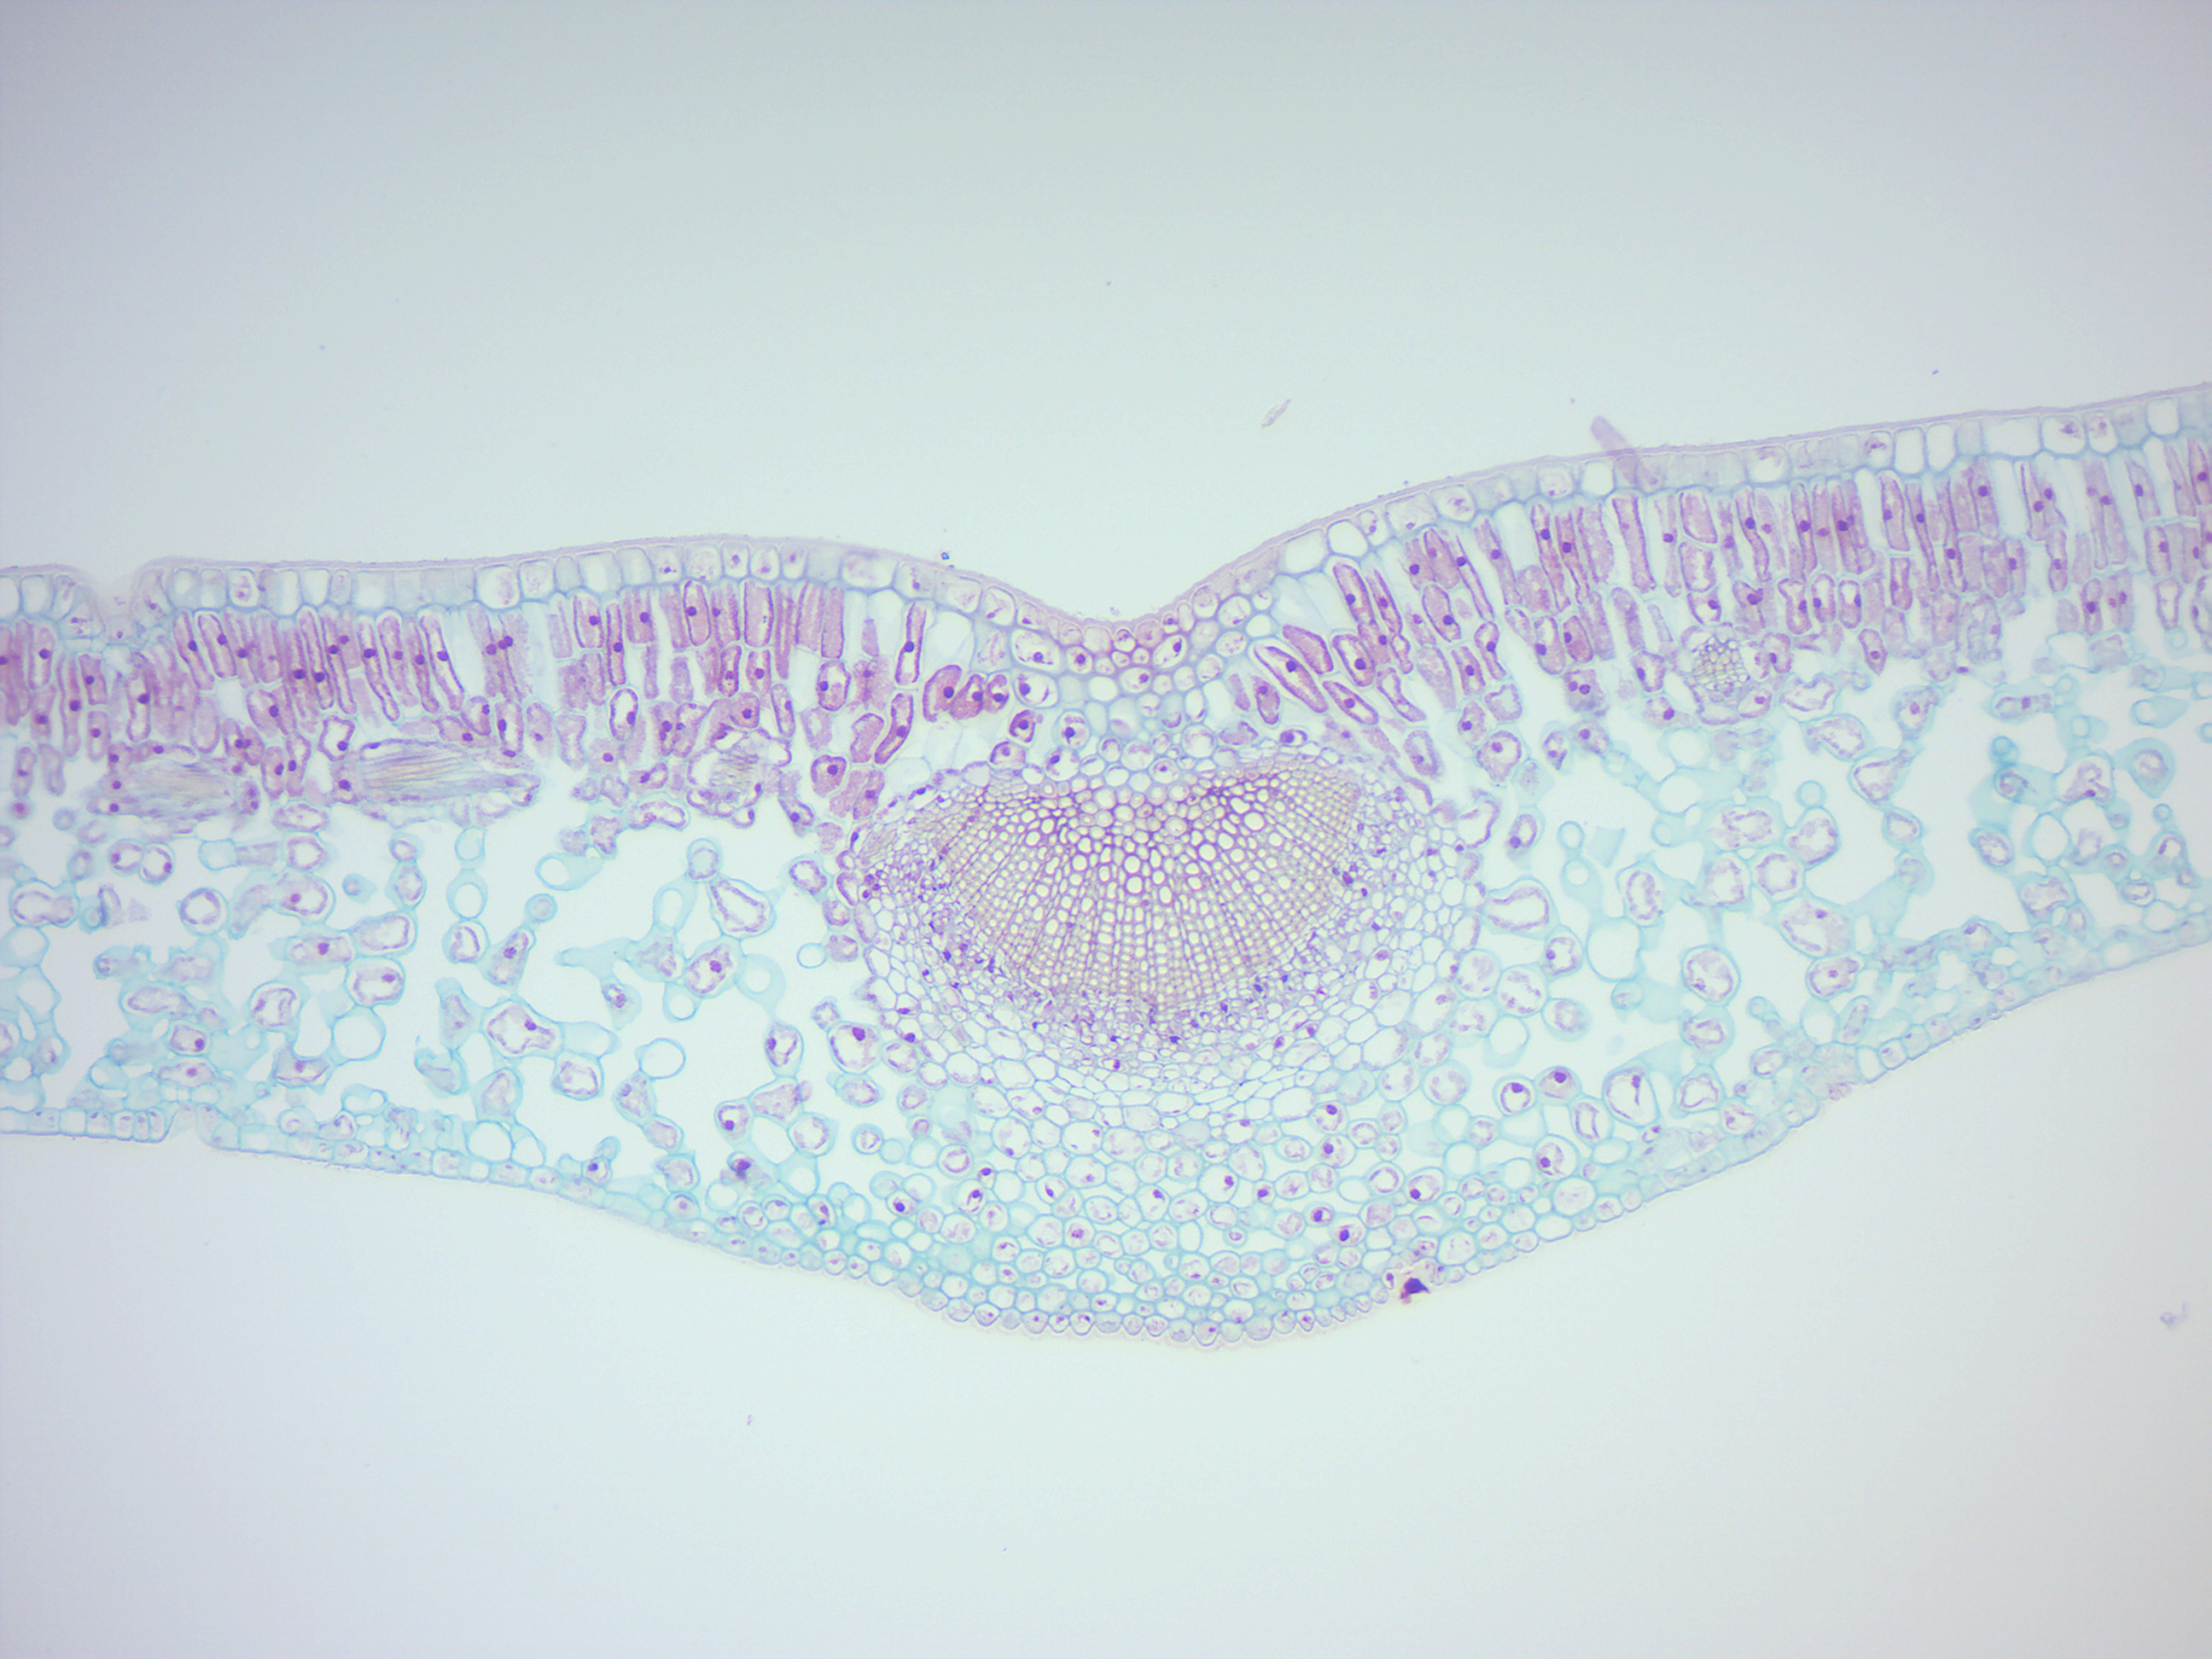
\includegraphics[width=0.7\linewidth]{./figures/gymnosperms/dicot_leave}

}

\caption{Dicot leave.}\label{fig:dicotleave}
\end{figure}

\begin{figure}

{\centering 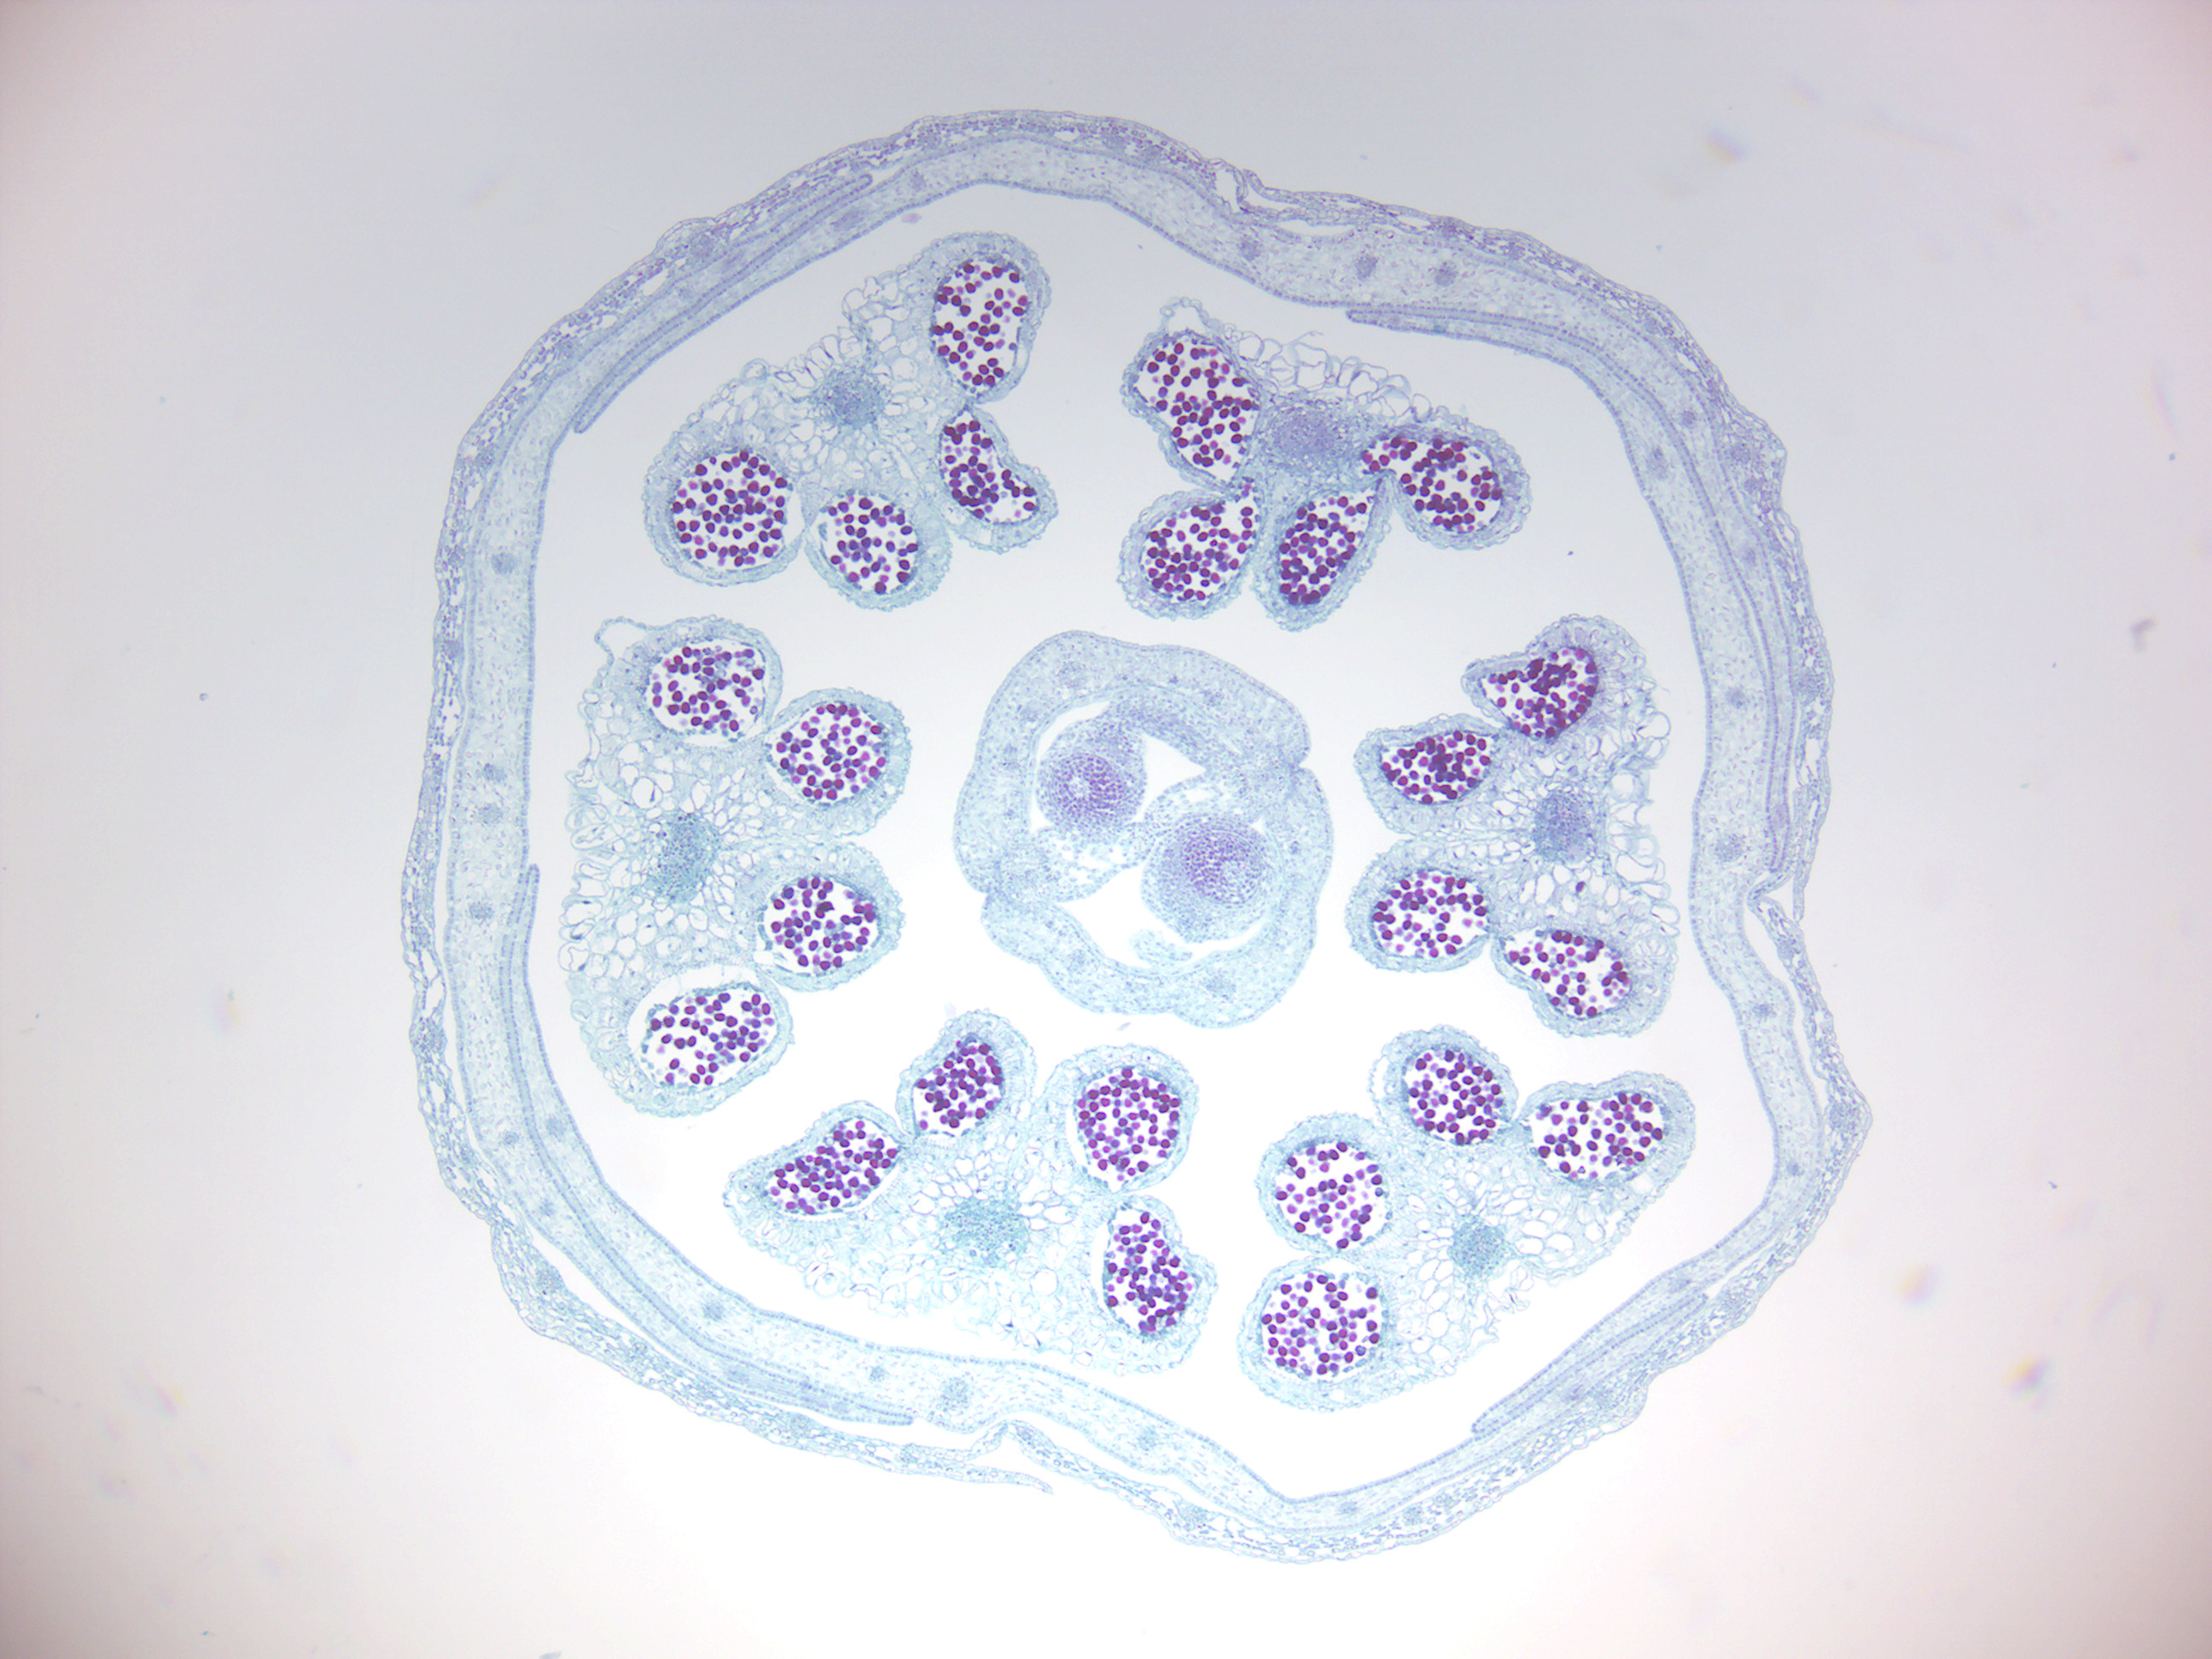
\includegraphics[width=0.7\linewidth]{./figures/gymnosperms/monocot_flower_bud}

}

\caption{Monocot flower bud.}\label{fig:monocotbud}
\end{figure}

\begin{figure}

{\centering 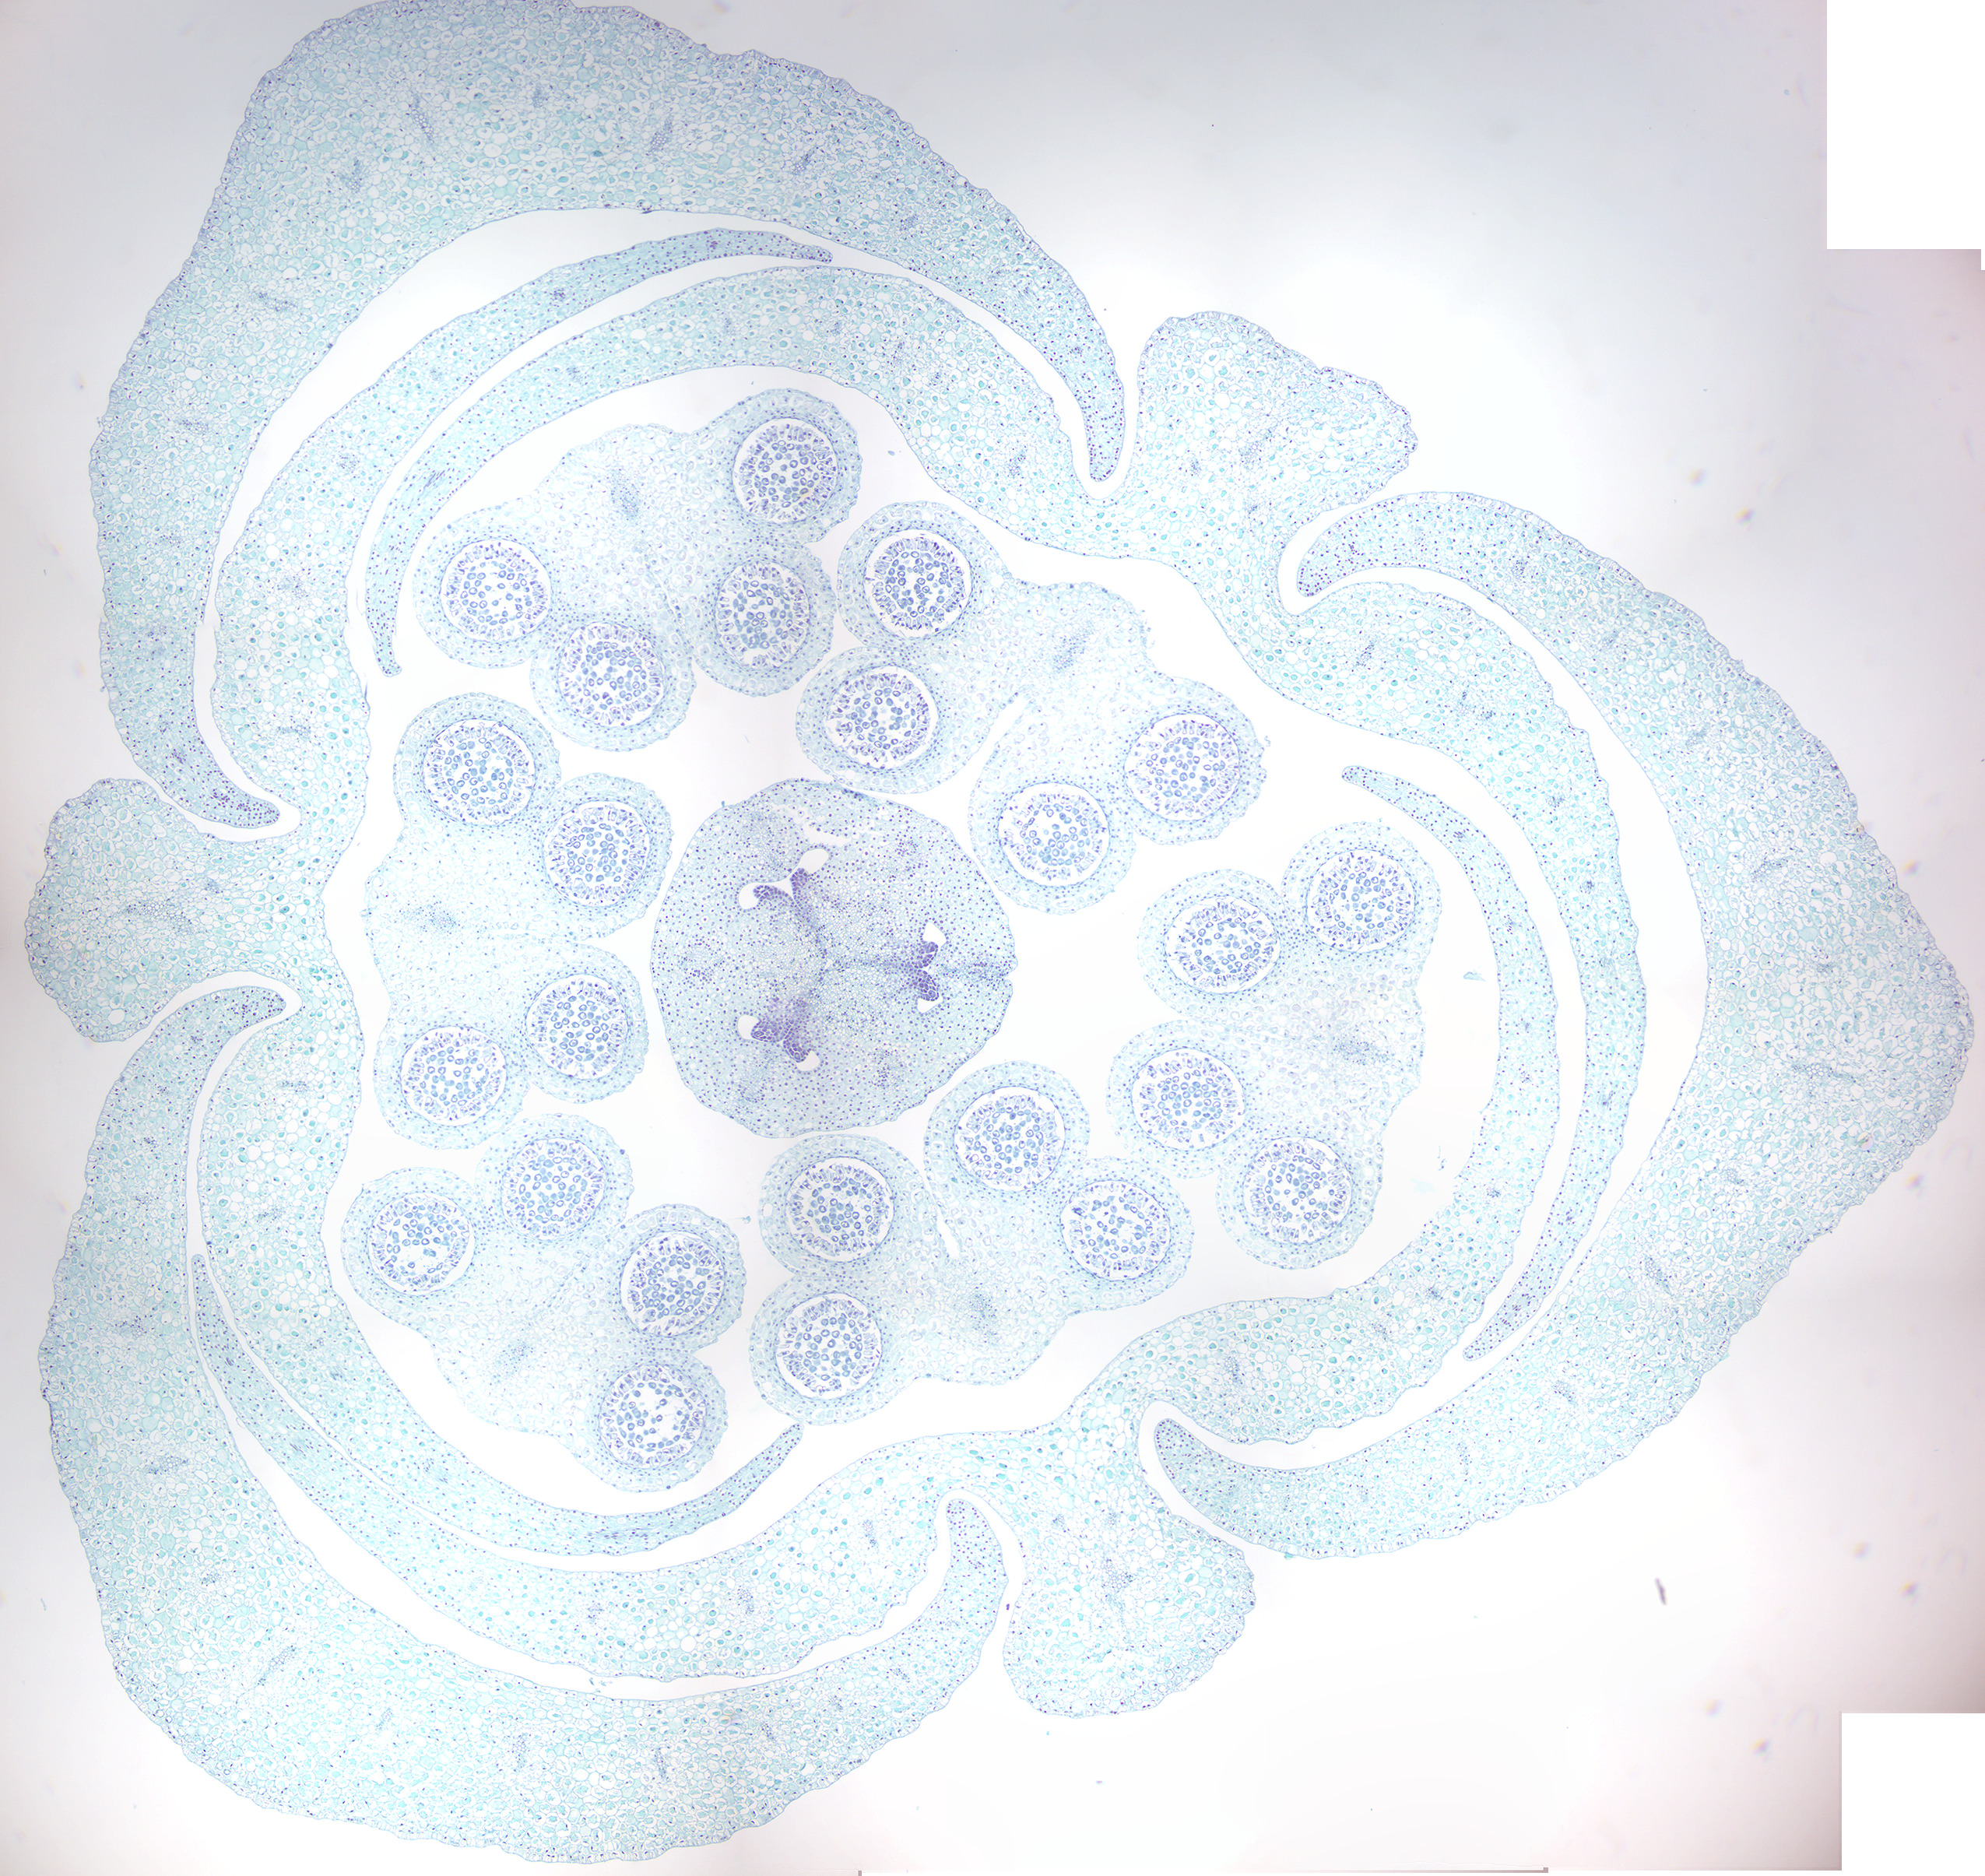
\includegraphics[width=0.7\linewidth]{./figures/gymnosperms/dicot_flower_bud}

}

\caption{Dicot flower bud.}\label{fig:dicotbud}
\end{figure}

\pagebreak

\section{\texorpdfstring{\emph{Lilium}}{Lilium}}\label{lilium}

\emph{Lilium} is a genus of herbaceous flowering plants growing from
bulbs, all with large prominent flowers. Lilies are a group of flowering
plants which are important in culture and literature in much of the
world. Most species are native to the temperate northern hemisphere,
though their range extends into the northern subtropics. Lilies are
tall perennials ranging in height from 2--6 ft.

\begin{figure}

{\centering 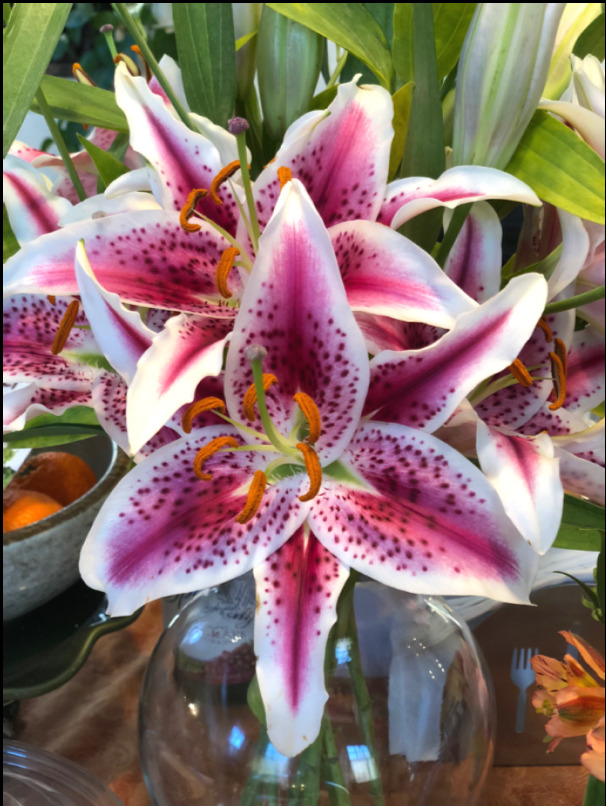
\includegraphics[width=0.7\linewidth]{./figures/gymnosperms/lily}

}

\caption{Lilies}\label{fig:Lilies}
\end{figure}

The flowers are large, often fragrant, and come in a wide range of
colors including whites, yellows, oranges, pinks, reds and purples.
Markings include spots and brush strokes. The plants are late spring- or
summer-flowering. Flowers are at the tip of the stem, with six tepals
(sepals and petals are not distinct). The tepals are free from each
other, and bear a nectary at the base of each flower. The ovary is
`superior', borne above the point of attachment of the anthers. The
fruit is a three-celled capsule. Seeds ripen in late summer. They
exhibit varying and sometimes complex germination patterns, many adapted
to cool temperate climates. 

\section{Dissection of Fresh Lilies}\label{dissection-of-fresh-lilies}

\begin{enumerate}
\def\labelenumi{\arabic{enumi}.}
\tightlist
\item
  The outer ring of the flower consists of sepals, and the inner ring of
  petals. In lilies they look nearly identical. In many other flowers,
  the sepals are green and the petals are colorful.
\item
  Peel off first the sepals and then the petals.
\item
  Count the number of sepals and petals. Do you notice any (orange
  colored) pollen on any of them?
\item
  After you have peeled away the sepals and petals, you can clearly see
  the stamens (the ``male'' parts of the flower). The stamens mostly
  consist of anthers (the long, elliptical and brown heads on top of the
  filaments (the supporting stalks). Some anthers may have split open to
  expose othe pollen grains inside.
\item
  Cut off the stamens and examine the anther and pollen using the stereo
  dissection microscope.
\item
  The long stalk remainin in the center of the flower is the pistil (the
  ``female'' parts) with the stigma at its top end. If the flowers are
  fresh, the stigma will be sticky for catching pollen. You can cut it
  open along the path down the style (the stalky part), to the ovule.
\item
  At the base of the style is the ovary. It contains the ovules that
  will develop into vseeds if they are fertilized by sperm from the
  pollen.
\item
  Cut the ovary in half to see the ovules.
\item
  Examine the cut ovary using the stereo dissection microscope.
\item
  At the base of the the ovary is the main nectary. Cut it open to see
  the xylem (the water conducting vessels of vascular plants) and phloem
  (the sugar conductiong vessels).
\end{enumerate}

\section{Review Questions}\label{review-questions-2}

\begin{enumerate}
\def\labelenumi{\arabic{enumi}.}
\tightlist
\item
  What are gymnosperms?
\item
  What are angiosperms?
\item
  What are pollen?
\item
  What are cotyledons?
\item
  What is xylem?
\item
  What is phloem?
\end{enumerate}

\end{document}
